%% FEUP THESIS STYLE for LaTeX2e
%% how to use feupteses (English version)
%%
%% FEUP, JCL & JCF, 31 July 2012
%%
%% PLEASE send improvements to jlopes at fe.up.pt and to jcf at fe.up.pt
%%

\documentclass[11pt,a4paper,twoside,openright]{report}

%% For iso-8859-1 (latin1), comment next line and uncomment the second line
%\usepackage[latin1]{inputenc}
\usepackage[utf8]{inputenc}
\usepackage[portuguese,english]{babel}
\selectlanguage{english}

%% MIEIC options
%\usepackage[mieic]{feupteses}
\usepackage[dvipsnames]{xcolor}
\usepackage{fancyvrb}
\usepackage[mieic,juri]{feupteses}
%\usepackage[mieic,final]{feupteses}
%\usepackage[mieic,final,onpaper]{feupteses}

%% Uncomment the next lines if side by side graphics used
%\usepackage[lofdepth,lotdepth]{subfig}
%\usepackage{graphicx}
\usepackage{float}
\usepackage[algochapter]{algorithm2e}
\usepackage{amsmath}
\usepackage{hyperref}

%% Macros file
%some macro definitions

% format
\newcommand{\class}[1]{{\normalfont\slshape #1\/}}

% entities
\newcommand{\Feup}{Faculdade de Engenharia da Universidade do Porto}

\newcommand{\svg}{\class{SVG}}
\newcommand{\scada}{\class{SCADA}}
\newcommand{\scadadms}{\class{SCADA/DMS}}


% Glossary
\usepackage{footnote}
\usepackage{array,multirow}
\usepackage{longtable}
\usepackage{tabu}
\usepackage[acronym,nonumberlist]{glossaries}
\makeglossaries
\chapter{Glossary}

This brief glossary was based on a similar work by Robert Lyons \cite{gloss}.

\begin{flushleft}
\begin{tabular}{l p{0.8\linewidth}}

cDNA                  & DNA which has been reverse transcribed using RNA as a
template.\\

Exon                  & The portions of a genomic DNA sequence which will be
represented in the final, mature mRNA. Exons may include coding sequences, the
\textit{5'} untranslated region or the \textit{3'} untranslated region.\\

Expression            & To \qt{express} a gene is to cause it to function. A gene
which encodes a protein will, when expressed, be transcribed and translated to
produce that protein. A gene which encodes an RNA rather than a protein (for
example, a rRNA gene) will produce that RNA when expressed.\\

Gene                  & A unit of DNA which performs one function. Usually, this
is equated with the production of one RNA or one protein. A gene contains coding
regions, introns, untranslated regions and control regions.\\

Genome                & The total DNA contained in each cell of an organism.
There are somewhere in the order of a hundred thousand genes, including coding
regions, \textit{5'} and \textit{3'} untranslated regions, introns, \textit{5'}
and \textit{3'} flanking DNA.\\

Intron                & Introns are portions of genomic DNA which are
transcribed (and thus present in the primary transcript) but which are later
spliced out. Thus, they are not present in the mature mRNA.\\

mRNA                  & \qt{Messenger RNA} contains sequences coding for a
protein. The term mRNA is used only for a mature transcript (with all introns
removed), rather than the primary transcript in the nucleus.\\

rRNA                  & \qt{Ribosomal RNA} describes any of several RNAs which
become part of the ribosome, and thus are involved in translating mRNA and
synthesizing proteins.\\

\end{tabular}
\end{flushleft}
\begin{flushleft}
\begin{tabular}{l p{0.8\linewidth}}

Shotgun cloning       & The process of randomly shearing an organism's genomic
DNA and cloning it into a suitable vector, resulting in a genomic library.\\

Shotgun sequencing    & Sequencing the DNA library created by shotgun cloning.\\

Transcription         & The process of copying DNA to produce an RNA transcript.
This is the first step in the expression of any gene. The resulting RNA will
produce the desired protein molecule by the process of translation.\\

Translation           & The process of decoding a strand of mRNA, thereby
producing a protein based on the code.\\

tRNA                  & \qt{Transfer RNA} represents one of a class of rather
small RNAs used by the cell to carry amino acids to the enzyme complex (the
ribosome) which builds proteins, using an mRNA as a guide.\\

\end{tabular}
\end{flushleft}


\chapter*{Abbreviations}
\chaptermark{ABBREVIATIONS}

\begin{flushleft}
\begin{tabular}{l p{0.8\linewidth}}
API       & Application Programming Interface\\
AUC       & Area Under the Curve\\
BLAST     & Basic Local Alignment Search Tool\\
cDNA      & Complementary DNA\\
CSS       & Cascading Style Sheets\\
DBMS      & Database Management System\\
DNA       & Deoxyribonucleic Acid\\
GUI       & Graphical User Interface\\
HTML      & HyperText Markup Language\\
IBMC      & Institute for Molecular and Cell Biology \textit{(Instituto de Biologia Molecular e Celular)}\\
ILP       & Inductive Logic Programming\\
K-NN      & K-Nearest-Neighbors\\
mRNA      & Messenger RNA\\
NCBI      & National Center for Biotechnology Information\\
NGS       & Next Generation Sequencing\\
RNA       & Ribonucleic Acid\\
RNA-Seq   & RNA Sequencing\\
ROC       & Receiver Operating Characteristic\\
SAM       & Sequence Alignment/Map\\
SVM       & Support Vector Machine\\
rRNA      & Ribosomal RNA\\
tRNA      & Transfer RNA\\
WTSS      & Whole Transcriptome Shotgun Sequencing\\
\end{tabular}
\end{flushleft}



%% Include color package
\usepackage{color}
\definecolor{cloudwhite}{cmyk}{0,0,0,0.025}

%% Create comments and notes
\usepackage{comment}
\definecolor{noteblue}{cmyk}{0.8,0.4,0,0}
\definecolor{notegreen}{cmyk}{0.31,0,0.44, 0.25}
\specialcomment{Notes}{
  \begingroup\Large\color{noteblue}\flushleft{NOTES}\endgroup\\
  \begingroup
    \color{noteblue}}
  {\endgroup}
\specialcomment{Structure}{
  \begingroup\Large\color{notegreen}\flushleft{STRUCTURE}\endgroup\\
  \begingroup
    \color{notegreen}}
  {\endgroup}
\excludecomment{Notes}
%\excludecomment{Structure}

%% Include source-code listings package
\usepackage{listings}
\lstset{%
language=C,                        % choose the language of the code
 basicstyle=\footnotesize\ttfamily,
 keywordstyle=\bfseries,
 numbers=left,                      % where to put the line-numbers
 numberstyle=\scriptsize\texttt,    % the size of the fonts that are used for the line-numbers
 stepnumber=1,                      % the step between two line-numbers. If it's 1 each line will be numbered
 numbersep=8pt,                     % how far the line-numbers are from the code
 frame=tb,
 float=htb,
 aboveskip=8mm,
 belowskip=4mm,
 backgroundcolor=\color{cloudwhite},
 showspaces=false,                  % show spaces adding particular underscores
 showstringspaces=false,            % underline spaces within strings
 showtabs=false,                    % show tabs within strings adding particular underscores
 tabsize=2,	                    % sets default tabsize to 2 spaces
 captionpos=b,                      % sets the caption-position to bottom
 breaklines=true,                   % sets automatic line breaking
 breakatwhitespace=false,           % sets if automatic breaks should only happen at whitespace
 escapeinside={\%*}{*)},            % if you want to add a comment within your code
 morekeywords={*,var,template,new}  % if you want to add more keywords to the set
}

% Gantt charts
\usepackage{pgf}
\usepackage{tikz}
\usetikzlibrary{shapes,arrows}
\usepackage{flafter}

% Font size
\usepackage[bitstream-charter]{mathdesign}
\usepackage[T1]{fontenc}

%% Uncomment to create an index (at the end of the document)
%\makeindex

%% Path to the figures directory
\graphicspath{{figures/}}

%%========================================
%% Start of document
%%========================================
\begin{document}

%%----------------------------------------
%% Information about the work
%%----------------------------------------
\title{A Computational Platform for Gene Expression Analysis}
\author{Diogo André Rocha Teixeira}

%% Uncomment next line for date of submission
\thesisdate{June 23, 2014}

%%Uncomment next line for copyright text if used
%\copyrightnotice{Name of the Author, 2008}

\supervisor{Supervisor}{Rui Camacho}
\supervisor{Second Supervisor}{Nuno Fonseca (EMBL-EBI, Cambridge, UK)}

%% Uncomment committee stuff in the final version if used
%\committeetext{Approved in oral examination by the committee:}
%\committeemember{Chair}{Doctor Name of the President}
%\committeemember{External Examiner}{Doctor Name of the Examiner}
%\committeemember{Supervisor}{Doctor Name of the Supervisor}
%\signature

%% Specify cover logo (in folder ``figures'')
\logo{uporto-feup.pdf}

%% Uncomment next line for additional text  below the author's name (front page)
%\additionalfronttext{Preparação da Dissertação}

%%----------------------------------------
%% Preliminary materials
%%----------------------------------------
\begin{Prolog}
  \chapter*{Abstract}

The advent of next generation sequencing methods has revolutionized the field of
molecular biology in the past few years. Following this theme, we will discuss
the usage of \rnaseq{} methods in order to understand how the final portion of
genetic code of a gene's exon affects the transcription speed of that same exon.
We will describe the several components of the information system that will be
developed to address this problem. A literature review will be presented, for
both the areas of transcriptome assembly and data mining, addressing the most
relevant concepts regarding our particular problem. Lastly, we will provide an
estimated work plan for the project development and describe the methods that
will be used for validating the project's results.

\chapter*{Resumo}

\begin{otherlanguage}{portuguese}
O advento das técnicas de sequenciação de nova geração revolucionou o campo da
biologia molecular nos últimos anos. Seguindo este tema, vamos discutir o uso de
métodos de \textit{\rnaseq{}} para perceber de que forma a porção final do
código genético do exão de um gene afeta a velocidade a velocidade de
transcrição desse mesmo exão. Vamos descrever os vários componentes do sistema
de informação que vai ser desenvolvido para endereçar este problema. Será
apresentada a revisão da literatura, nas áreas de assemblagem de \textit{RNA} e
\textit{data mining}, endereçando os conceitos mais relevantes relativamente ao
nosso problema particular. Por fim, vamos apresentar uma estimativa para o plano
de trabalho para o desenvolvimento do projeto e descrever os métodos que serão
usados para a validação dos resultados do projeto.
\end{otherlanguage}
 % the abstract
  \chapter*{Acknowledgements}

First of all, I would like to direct my gratitude to my supervisor, Rui Camacho
(FEUP). His concern about my work and the helpfulness he has always shown were
key factors for the success of this project. I extend the same gratitude to my
co-supervisor, Nuno Fonseca (EMBL-EBI), for his endless patience in answering my
questions.

I would also like thank Alexandra Moreira, Andrea Cruz and Jaime Freitas (IBMC)
for the fantastic way they always welcomed me. Their willingness to help me
through the difficult of learning a completely new field of study was
fundamental to my progress.

A very special thank you to my all my friends at FEUP, that were with me in what
is surely one of the best periods in my life. In particular I would like to
acknowledge Pedro. Our constant competition, along with our shared antics, made
working on this project that much more fun and fulfilling.

To my parents, Joaquim and Maria, I leave a truly heartfelt thank you; for all
the nights they spent awake worrying about me; for all their guidance and
wisdom; for being with me in every good and bad moment of my life. I would not
be the person I am today without them.

Lastly, but definitely not least, I thank my girlfriend, Raquel. Of everything I
have and owe to her, nothing is more important than the smile she puts on my
face every day, as she gives me the strength to face the world.

\vspace{10mm}
\flushleft{Diogo Teixeira}
  % the acknowledgments
  \cleardoublepage
\thispagestyle{plain}

\vspace*{8cm}

\begin{flushright}
   \textsl{``You should be glad that bridge fell down. \\
           I was planning to build thirteen more to that same design''} \\
\vspace*{1.5cm}
           Isambard Kingdom Brunel
\end{flushright}
       % initial quotation if desired
  \cleardoublepage
  \pdfbookmark[0]{Table of Contents}{contents}
  \tableofcontents
  \cleardoublepage
  \pdfbookmark[0]{List of Figures}{figures}
  \listoffigures
  \cleardoublepage
  \pdfbookmark[0]{List of Tables}{tables}
  \listoftables
  \pdfbookmark[0]{List of Algorithms}{algorithms}
  \listofalgorithms
  \printglossary[type=acronym,title=Abbreviations]
\end{Prolog}

%%----------------------------------------
%% Body
%%----------------------------------------
\StartBody

%\begin{Notes}
%- Add glossary and abbreviations.\\
%\end{Notes}

\chapter{Introduction} \label{chap:intro}

\section*{}

\section{Context and Motivation} \label{sec:context}

\section{Objectives} \label{sec:goals}

While defining the concrete objectives of this thesis it becomes relevant to
separate them in two groups: strictly biology research related objectives and
more general, software solution development objectives. Despite this division,
both objectives are tightly interconnected, and each complements the other.

From a molecular biology standpoint, the main objective of this thesis will be
to try to understand the mechanisms that regulate the speed of transcription for
coding regions of the \dna. This information will be obtained using the
\rnaseq{} method, that will be further discussed in chapter \ref{chap:sota}.
There are several intermediate objectives for this particular problems, as
follows:

\begin{itemize}

  \item
  Alignment of the given sequencing reads into a known reference genome. This is
  one of the first steps in the \rnaseq{} process and is effectively one of the
  most complex problems addressed by this thesis. Some of the tools used in this
  particular step of the process will be referenced in section \ref{sec:seqtools}.

  \item
  Further analysis of the \rnaseq{} results using machine learning algorithms,
  applied to data mining. These techniques will be used in an effort to try to
  understand the already mentioned transcription mechanisms. This topic will be
  developed in section \ref{sec:mlearning}.

\end{itemize}

The last objective of this thesis is the development of a software platform
prototype. This prototype comes as a materialization of the work done along the
previous objectives, combining the developed genetic data processing pipeline,
with a web information system and with data mining tools. When completed, the
prototype should allow for users to store, search and manipulate their genome
sequencing data. This data can them be assembled using the tool pipeline
developed for the analysis of our own experimental dataset. Lastly, the
prototype should integrate data mining tools, that would allow users to
reproduce the types of data analysis that were done in this thesis, on their own
results.

This document, however, will not dwell in the details of the implementation of
such a platform, but rather in the molecular biology section of the overall
problem. This is largely due to the fact that the development of the web
platform is highly dependent on the tools and methods that will be used for
tackling the biology aspects of the problem and, as such, is likely to suffer
significant alterations.

\section{Document Outline} \label{sec:outline}

Besides the introduction chapter, this document is composed three additional
chapters. These chapters have the following structure:

\begin{description}

  \item[Chapter \ref{chap:sota}]
  introduces some basic Biology and \rnaseq{} concepts, that are essential to
  understand the problems with which this document deals. Furthermore, we
  describe the main techniques used for genome/transcriptome sequencing and
  assembly, their differences and applications and the tools and data formats
  typically used on those areas. Lastly, we give some insight about machine
  learning algorithms and how they will be applied to this work.

  \item[Chapter \ref{chap:validation}]
  presents the datasets that will be studied and used in this work, their
  origins and features. We will also refer the validation methods that will
  be used to access the quality of our results.

  \item[Chapter \ref{chap:workplan}]
  outlines the main steps in the development of this thesis (and the respective
  software prototype). In the last part of this chapter we will attempt to
  provide a feasible schedule for this work's execution.

\end{description}

\chapter{State-of-the-Art} \label{chap:sota}

\section*{}

%\begin{Notes}
%- Change transcriptome assembly to read alignment.\\
%\end{Notes}

In this chapter we will begin by making a more in depth presentation of the
process of gene expression. This will be followed by a literature and state of
the art review in the fields of read alignment, differential expression analysis
and data mining. We will present the tools used in the development of the
analysis pipelines and the web platform. Lastly, we review some result
evaluation techniques and relevant data representation formats for genetic
information.

\section{Biological Base Concepts}

%\begin{Notes}
%- Base concepts look good.\\
%- Include part about RNA binding proteins.\\
%\end{Notes}

Before dwelling in the details of the state of the art that are on the
foundation of the thesis, it is important to explain some concepts of the
domain of molecular biology.

\subsection{Gene Expression}

As explained in Chapter \ref{chap:intro}, gene expression is the mechanism by
which an organism's \dna{} can be expressed into functional genetic products,
like proteins. This process starts with the genetic code, or nucleotide
sequence, of each gene. Different genes in an organism's \dna{} are responsible
for the creation of different genetic products. The process of gene expression
itself is composed by two main stages, transcription and translation
\cite{leic:gene_expr}.

Transcription is the stage at which genetic data in the form of \dna{} is used
to synthesize \rna{}, being this the process that concerns the thesis' main
question. Several different types of \rna{} are produced by this process,
including mRNA (which specifies the sequences of amino acids that form a
protein), rRNA and tRNA, both later used in the translation stage. Simplifying
a gene's structure, it can be seen as composed by two types of sequences,
introns and exons, as seen in Figure \ref{fig:intron_exon}.

\begin{figure}[!htb]
  \begin{center}
    \leavevmode
    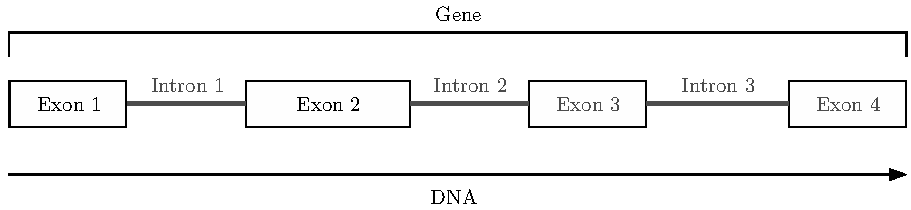
\includegraphics[width=1.0\textwidth]{intron_exon2}
    \caption[Overall structure of a gene]{Overall structure of a gene, with its
    different areas (simplified).}
    \label{fig:intron_exon}
  \end{center}
\end{figure}

The exons are useful in the gene expression process, being also known as coding
regions. Introns, on the other hand, are not used in the process. They are
present in an early stage mRNA molecule, the precursor mRNA, but are later
removed (or spliced) in the final molecule before the translation stage
\cite{leic:gene_expr}. Figure \ref{fig:splicing} illustrates the removal of
introns from the mRNA molecule, during the  splicing process.

\begin{figure}[!htb]
  \begin{center}
    \leavevmode
    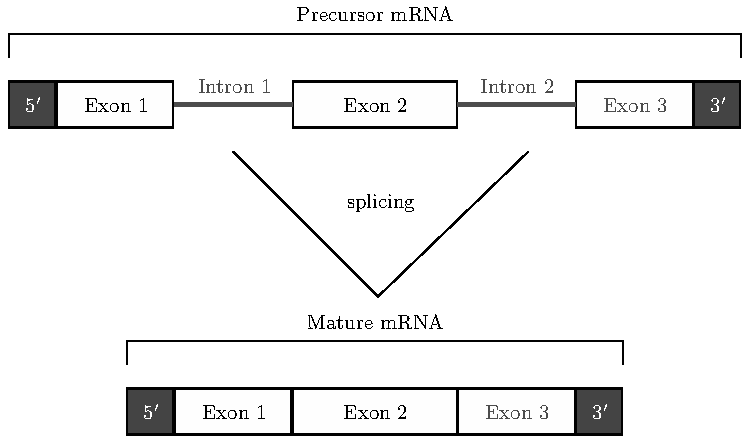
\includegraphics{splicing2}
    \caption[Removal of introns from precursor mRNA]{The removal (splicing) of
    introns from the precursor mRNA, during the transcription process.}
    \label{fig:splicing}
  \end{center}
\end{figure}

After the conclusion of the transcription process comes the translation process.
In this process, the synthesized mRNA is used to specify the sequence of amino
acids that constitute the particular protein being produced. The other types of
RNA molecules (rRNA and tRNA) are also used in this stage of the gene expression
process.

\subsection{RNA-Binding Proteins}

RNA-binding proteins, also referred to as RBP, regulate every aspect of the RNA
metabolism, including pre-mRNA splicing, mRNA transport, location, stability and
translation control \cite{Cooper2009777, Muller-McNicoll2013, Sonenberg2007721,
Sonenberg2009731}, as shown in Figure \ref{fig:rbp}.

\begin{figure}[!htb]
  \begin{center}
    \leavevmode
    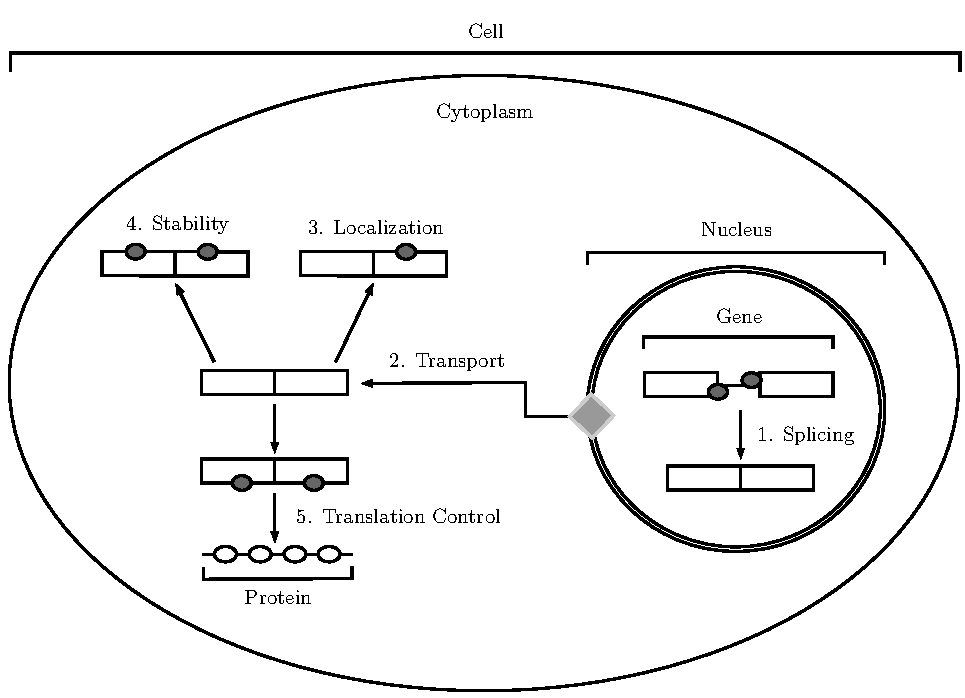
\includegraphics[width=\textwidth]{rbp}
    \caption[Role of RBPs in the RNA metabolism process]{
      Diagram of a typical cell showing the multiple roles of RBPs in post
      transcriptional processes \cite{janga2011construction}. The grey ellipses
      represent RBPs. The numbered text represents the different processes in
      which RBPs take part. Multiple RBPs can bind with a single RNA at one or
      more locations, creating an abundance of different combinations and
      possibilities in every step of the RNA metabolism.
    }
    \label{fig:rbp}
  \end{center}
\end{figure}

The binding of RBPs to RNA depends on different RNA-sequence specificities and
affinities. This aspect, coupled with the existence of hundreds of RBPs in an
organism, gives rise to a plethora of different combinations and outcomes to the
RNA metabolism.

RBPs regulate gene expression in health and disease, and mutations affecting the
function of RBPs may cause several diseases \cite{Cooper2009777}. Therefore,
understanding the binding patterns of RBPs during a particular biological
process is crucial to get insight into that process, both during health and
disease conditions.

\subsection{Sequencing}

Obtaining genetic information is done experimentally, by employing a sequencing
technique. For quite some time this process was carried out using the Sanger's
and other similar sequencing methods methods \cite{Reis-Filho2009}. Though
effective, such methods were notably slow and costly, with large projects like
the Human Genome Project (HGP) consuming roughly thirteen years and US\$ 3
billion. These limitations were so severe that, other than the realm of human
genetics, this kind of study was restricted to model organisms, such as the
fruit fly and mouse genomes \cite{Wolf2013}. The past few years have seen the
appearance and rise in popularity of the \ngs{} techniques. These techniques
differ from the more classical ones by producing larger amounts of information,
at lower cost. They are also typically more cost effective than previous
techniques and can be easily employed by single laboratories, which has greatly
contributed to their popularity.

The rise in popularity and availability of \ngs{} techniques, coupled with the
importance of RNA knowledge in understanding gene expression, led to the
appearance of RNA-Seq. RNA-Seq makes use of these newly available
deep-sequencing techniques to profile complete transcriptomes. This is, however,
a difficult task to accomplish. \ngs{} techniques produce shorter reads than
their older counterparts, being that \qt{\textit{(...) transcriptome assembly
from billions of RNA-Seq reads (...) poses a significant informatics challenge}}
\cite[p. 671]{Martin2011}.

Although this thesis does not deal with the problems of sequencing techniques, it
is important to indicate that the read data sets that were used resulted from
\ngs{} techniques, in particular RNA-Seq. As such, suitable tools for this
particular type of data were used.

\subsection{\Trans{} Assembly}

\Trans{} assembly is the process by which experimentally obtained RNA data reads
can be organized and merged together in a partial or complete \trans. As stated
above, the advent of next generation sequencing techniques, with their reduced
costs, greatly increased the availability of transcript sequencing data.

For years, microarrays were the standard tool available for examining features
of the transcriptome and global patterns of gene expression \cite{Wolf2013}.
However, microarrays are typically more oriented towards assembly against
existing reference data, hence limiting its application to species with well
known reference genomes. This is impractical, as \ngs{} techniques allow to
cheaply obtain genetic information of previously non-studied species. This is
one of the reasons that led to the inception of RNA-Seq. Contrary to
microarrays, RNA-Seq techniques are able to wield results that are suitable for
both reference guided assembly and \textit{de novo} assembly approaches
\cite{Wilhelm2009}. \textit{De novo} or exploratory assembly has captured the
interest of researchers in the past few years, leading to the appearance of
multiple RNA-Seq tools that are capable of making this type of assembly without
a reference genome \cite{nuno11:assemblathon}. Transcriptome assembly was not
performed during this thesis, as its main focus in terms of the RNA-Seq process
is read alignment and differential expression analysis.

\section{RNA-Seq Analysis}

\begin{Notes}
- Describe the same workflow as iRAP.\\
- Refer that we'll talk about specific tools below, and they all are Unix
command line tools.
\end{Notes}

\subsection{RNA-Seq Pipeline}

\begin{figure}[!htb]
  \begin{center}
    \leavevmode
    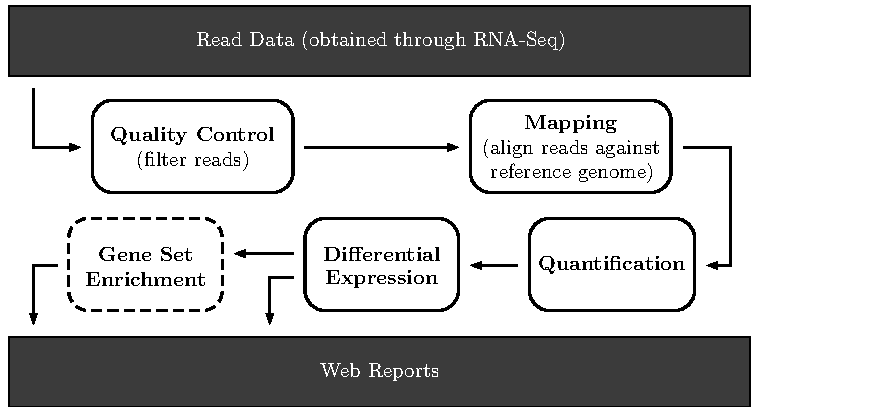
\includegraphics{irap}
    \caption[iRAP RNA-Seq data analysis pipeline]{
      iRAP RNA-Seq data analysis pipeline. Note that the gene enrichment step
      (in dashed line) is optional and was not used.
    }
    \label{fig:irap}
  \end{center}
\end{figure}

\subsection{\rnaseq{} Read Alignment and Analysis Tools}

Below we present some bioinformatic tools, used to support the multiple steps of
the \rnaseq{} read alignment and data analysis process. It is important to note that none of these
tools were used separately, but rather as parts of an analysis pipeline (also
described below).

\subsubsection*{Tuxedo Suite}

The Tuxedo suite is a free, open-source collection of applications that has been
widely adopted as analysis toolset for fast alignment of short reads. It is
composed by four separate tools, Bowtie, TopHat, Cufflinks and CummRbund,
briefly reviewed below. These tools are extensively used for \rnaseq{} analysis.
Although the applications are made for command line execution, there are several
workflow managers, like Galaxy\footnote{\url{http://galaxyproject.org/}}, that
easily integrates with the suite, providing a web interface for its use. Note
that not all components of the Tuxedo Suite were used.

\paragraph{Bowtie}

Bowtie is an ultrafast, memory-efficient short read aligner
\cite{langmead2009ultrafast}. Bowtie is typically used to build a reference
index for the genome of the organism being studied, for posterior use by other
tools, like TopHat. It can also output alignments in the standard SAM format,
allowing Bowtie to interoperate with tools like SAM Tools. However, it should
not be used as a general purpose alignment tool, as it was created and is more
effective when aligning short read sequences against large reference genomes.

\paragraph{TopHat}

TopHat is a fast splice junction mapper for \rnaseq{} reads
\cite{Trapnell01052009}. It uses Bowtie as the underlying alignment tool, using
its results and a FASTA formated reference genome to identify splice junctions
between exons.

\paragraph{Cufflinks}

Cufflinks assembles transcripts, estimates their abundances, and tests for
differential expression and regulation in \rnaseq{} samples
\cite{trapnell2010transcript}. It uses the SAM or BAM formatted files as input,
typically the ones produced by TopHat, outputting GTF files as a result.

\paragraph{CummeRbund}

Lastly, CummeRbund\footnote{\url{http://compbio.mit.edu/cummeRbund/}} is an R
package (see Section \ref{sec:mintools}) designed to help the visualization and
analysis of Cufflinks' \rnaseq{} output. As such, it is not directly involved in
the trascriptome alignment process. It takes the various output files from
Cufflinks and uses them to build a SQLite database describing appropriate
relationships between genes, transcripts, etc. This database is later used to
convert that data to R objects which allows them to be used the included
plotting functions, as well as in other commonly used data visualizations.

\subsubsection*{HTSeq}

HTSeq is a programming framework used for processing data resulting from next
generation sequencing methods \cite{htseq}, developed in Python. While many
tools can efficiently align reads, sometimes data needs to be manipulated before
being passed to those tools. This data can either be badly formated (or
\qt{dirty}) or simply in a format different from the one that is needed. The
latter is a particularly common problem when trying to pass the results of one
tool to the one that succeeds it in the pipeline. HTSeq is useful to easily
create scripts that accomplish this task, acting as a \qt{glue} between tools.

HTSeq provides parsers for many popular formats for representing genetic
information (see Section \ref{sec:formats}). In addition, it ships with two
standalone scripts, HTSeq-QA and HTSeq-Count. HTSeq-QA is used to provide an
initial assessment of the quality of sequencing runs, producing plots with that
information. HTSeq-Count takes a SAM/BAM file and GTF/GFF file containing gene
models. It then counts, for each gene, how many aligned reads overlap that
gene's exons.

\subsection{Differential Expression Analysis Tools}

Below we describe the tools that were used for differential expression analysis.
These tools are integrated in the iRAP pipeline, and make are used in its fourth
stage.

\subsubsection*{DESeq}

DESeq in an R package (see Section \ref{sec:mintools}), included in the
Bioconductor super package \cite{20979621}. DESeq takes count data generated
from RNA-Seq analysis assays. As count data is discrete and skewed, it is not
well approximated by a normal distribution. DESeq solves this problem by
applying a test based on the negative binomial distribution, which can reflect
these properties. This method has a much higher power to detect differential
expression.

\subsubsection*{edgeR}

edgeR in an R package (see Section \ref{sec:mintools}), included in the
Bioconductor super package \cite{robinson2010edger}. It provides methods for the
statistical analysis of count data from comparative experiments on next
generation sequencing platforms, among which is RNA-Seq, the most common source
of data used with edgeR. It has many characteristics in common with the
previously mentioned DESeq, as it also uses negative binomial models (among
others) to distinguish biological from technical variation. Later we describe
how both tools can be used together to produce better results.

\subsection{File Manipulation and Pre-processing Tools}

Sometimes data is badly formated or otherwise in a format that is not compatible
with a specific tool. This is particularly frequent when passing data between
two different tools in a pipeline. As such, we need some intermediate tools that
are able to easily manipulate and transform data, making it useful again. Below
we present some tools that can be used to accomplish this task.

\subsubsection*{SAM Tools}

SAM Tools\footnote{\url{http://samtools.sourceforge.net/}} is a library
package designed for parsing and manipulating alignment files in the SAM/BAM
format \cite{Li2009} (see Section \ref{sec:formats}). SAM Tools has two separate
implementations, one in C and the other in Java, with slightly different
functionality. Beyond manipulation of SAM and BAM files, this package is able to
convert between other read alignment formats, sort and merge alignments and show
them in a text-based viewer.

\subsubsection*{BLAST}

BLAST\footnote{\url{http://blast.ncbi.nlm.nih.gov/Blast.cgi}} is a tool,
implemented in C++, that is used to find regions of local similarity between
biological sequences. It uses FASTA sequences (see Section \ref{sec:formats}) as
search input and outputs the results reports in XML, HTML or plain text. There
are several different BLAST programs available at the moment, that can be used
depending on our objective and type of data. BLAST is particularly useful to
search biologic sequence databases, but can be used for other purposes, like
identifying an unknown species or comparing common genes in two related
species.

\subsubsection*{FASTX}

\subsubsection*{FastQC}

\subsection{Relevant Standard File Formats}\label{sec:formats}

As expected, the great diversity of RNA-Seq tools brings with it a wealth of
file formats. Some of these formats are developed from the ground up to satisfy
a specific need, while others are mere contextual adaptations or specializations
of already established formats. Below we will present a few of the most popular
and widely spread file formats, talking about their basic structure, the types
of data they represent and their applications.

\subsubsection*{FASTA}

FASTA is the standard line and character sequence format used by NCBI
\cite{ncbi:fasta}, using this last organization's character code conventions. It
is a simple format, that can be used to easily store data represented by
character sequences, like nucleotide (\dna, \rna) or amino acid (protein)
sequences. This file format is widely use to store sequencing reads, \dna/\rna{}
sequences and other character sequences in database systems. Its simplicity
makes it extremely easy to manipulate and parse, presenting also an attractive
solution for data transfer between different tools.

\subsubsection*{FASTQ}

FASTQ is used to store store character sequences, typically nucleotide sequences
\cite{Cock2010}. It is quite similar to the standard FASTA format, in respect to
the manner in which character sequences are represented. However, for every
sequence, there is a second sequence of equal length, representing the quality
scores of the original sequence. These quality scores are also represented as
single characters, taking values between and including ASCII-33 to ASCII-126.
It is typically used in the same situations as the FASTA format, when quality
scores are available/relevant.

\subsubsection*{SAM and BAM}

The SAM format is a text format for storing sequence alignment data
\cite{genome:sam}. It is widely used to store mapping information between
sequencing reads and a given reference genome. This sort of information is
typically the product of sequencing alignment tools, that consume sequencing
reads from FASTQ files and align them with a reference genome.

The BAM format contains exactly the same information as the SAM format and the
same rules apply for both formats. The difference between both formats lies in
their encoding. While SAM is a text based format, BAM is a binary format. This
means that BAM sacrifices human readability for increased machine processing
performance, as it is more efficient to work with compressed and indexed binary
data.

\subsubsection*{VCF}

VCF is a text file format used to store gene sequence variants \cite{smith13}.
In the past few years, as larger and larger genome sequencing projects became
more common (like the 1000 Genomes Project\footnote{The 1000 Genomes Project,
started back in 2008, is an international effort to establish the most
comprehensive catalogue to date of human genetic variations.}), storing such
large amounts of information became a serious concern. To address these concerns
the VCF format was created. Instead of storing the complete genome, VCF stores
only the variations (and their respective positions) of newly sequenced genomes
relatively to a known reference genome, typically in a compressed text file. As
such, it is a format often used when building genome databases.

\subsubsection*{GFF and GTF}

GFF is a text based file format to store gene features \cite{sanger11}. Many
genome assembly tools execute this process in two separate steps: feature
detection for identification of specific regions (exons, introns, etc.) and
genome assembly, using those features as reference. However, often times it is
beneficial to decouple these two steps, using different and more efficient tools
for each. As such, the GFF format emerged as a protocol for feature information
transfer between tools.

The GTF format is similar to the GFF format, in which it is based. It is also
used in similar situations. However, GTF builds on top of GFF, defining
additional conventions, specific to the domain of genetic information. Despite
their initial relation, both formats continue to be developed individually.

\section{Data Mining}\label{sec:mlearning}

\begin{Notes}
- Still relevant, don't change.\\
- Important part is now clustering, not classification.
\end{Notes}

Data mining is the process of \qt{\textit{extracting or \qt{mining} knowledge
from large amounts of data}} \cite[p. 5]{han2006data}. As such, it consists of a
set of techniques that can be used to find interesting patterns in large data
sets, that translate in newfound knowledge. Data mining borrows techniques from
multiple fields, such as artificial intelligence, machine learning, statistics,
and database systems \cite{Chakrabarti2012}. Its ultimate goal is to combine all
those techniques and transform large and (apparently) meaningless sets of data
into understandable and useful information. Thus, data mining was motivated by
the perspective of harnessing the abundance of data, that characterizes today's
information systems, to produce meaningful knowledge.

Because of their large quantities of input data, data mining tasks are usually
totally, or at least partially, automated. As such, there are several algorithms
for these tasks and tools that implements such algorithms, as presented in
Section \ref{sec:minalgo} and Section \ref{sec:mintools}, respectively.

We can divide data mining into main types: descriptive data mining and
predictive data mining \cite{Fayyad1996}. Descriptive data mining is focused on
finding the underlying structure of a given set of data. Instead of predicting
future values, it concerns the intrinsic structure, relations and
interconnectedness of the data being analyzed, presenting its interesting
characteristics without having any predefined target. On the other hand,
predictive data mining is used to predict explicit values, based on patterns
determined from the dataset. With predictive data mining we try to build models
using known data and use those models as a base to predict future behavior.

As we're seeing, data mining does not represent a single type problem. In fact
there are several different types of problems that can be addressed by data
mining techniques. Each of these problems may require a different data mining
method. A brief review of the most common methods is given below.

\begin{description}

  \item[Classification]
  is a method that tries to generalize the already known structure of a
  dataset, so that it applies to new datasets. In other words, with
  classification we try to learn a function that is capable of mapping our data
  into predefined classes.

  \item[Regression]
  tries to learn a function that models relationships between variables in the
  dataset. That function can latter be used to find real value predictions of
  future behavior of the same or similar datasets.

  \item[Clustering]
  consists in identifying a finite set of categories or clusters of similar
  values, to describe the dataset. As such, it is used without prior knowledge
  about data structure.

  \item[Summarization]
  provides a more compact representation of a subset of data, in a way that the
  summarized data retains the central points of the original data. This can be
  accomplished in several different ways, like using report generation or
  multivariate visualization techniques.

  \item[Dependency modeling]
  finds a model which describes relationships between variables, revealing their
  dependencies.

  \item[Change and deviation detection]
  tries to discover the most significant changes in the data, when compared with
  previously measured data. This method is useful to find interesting data
  variations or data errors.

\end{description}

\subsection{Data Mining Algorithms}\label{sec:minalgo}

\begin{Notes}
- Focus is now on clustering algorithms.
- See Wikipedia's page on "clustering" for a good reference on algorithm types.\\
\end{Notes}

In this project we will be concerned with the classification side of data
mining. Below, we will review some algorithms that can be used in
classification problems.

%\subsubsection*{Decision Trees}

%\textit{\qt{A decision tree is a flowchart-like tree structure, where each
%internal node (nonleaf node) denotes a test on an attribute, each branch
%represents an outcome of the test, and each leaf node (or terminal node) holds a
%class label}} \cite[p. 291]{han2006data}, as seen in Figure \ref{fig:tree}.
%Decision tree learning algorithms use a decision tree as a predictive model,
%that maps observed data about an individual to conclusions about the expected
%value for that individual. From a classification problem standpoint, this means
%means creating a decision tree structure that is able to predict the class of an
%individual based on its attributes.

%\begin{figure}[htb]
  %\centering

  %% Node levels and identation.
  %\tikzstyle{level 1}=[level distance=1.5cm, sibling distance=4.25cm]
  %\tikzstyle{level 2}=[level distance=1.5cm, sibling distance=2.25cm]
  %\tikzstyle{level 3}=[level distance=1.5cm, sibling distance=4.25cm]
  %\tikzstyle{level 4}=[level distance=1.5cm, sibling distance=2.25cm]

  %% Node style.
  %\tikzset{decision/.style={
    %draw=black!80, solid, fill=white!10, rectangle,
    %anchor=north,
    %inner sep=2mm, outer sep=0, text centered, growth parent anchor=south}
  %}
  %\tikzset{prediction/.style={
    %draw=black!80, solid, fill=white!30, ellipse,
    %anchor=north,
    %inner sep=2mm, outer sep=0, text centered, growth parent anchor=south,
    %minimum height=1cm,minimum width=1.3cm}
  %}

  %% Tree.
  %\begin{tikzpicture}
    %\node [decision] {\textit{age?}} [solid, -latex, thick, -]
      %child {
        %node [decision] {\textit{student?}} [solid, -latex, thick, -]
        %child {
          %node [prediction] {no} [solid, -latex, thick, -]
          %edge from parent
          %node[left] {no}
        %}
        %child {
          %node [prediction] {yes} [solid, -latex, thick, -]
          %edge from parent
          %node[right] {yes}
        %}
        %edge from parent
        %node[above left] {youth}
      %}
      %child {
        %node [prediction] {yes} [solid, -latex, thick, -]
        %edge from parent
        %node[below,fill=white,inner sep=1pt] {middle\_aged}
      %}
      %child {
        %node [decision] {\textit{credit\_rating?}} [solid, -latex, thick, -]
        %child {
          %node [prediction] {no} [solid, -latex, thick, -]
          %edge from parent
          %node[left] {no}
        %}
        %child {
          %node [prediction] {yes} [solid, -latex, thick, -]
          %edge from parent
          %node[right] {yes}
        %}
        %edge from parent
        %node[above right] {senior}
      %}
    %;
  %\end{tikzpicture}
  %\caption[Example of a decision tree]
  %{Example of a decision tree for the concept \textit{buys\_computer},
  %indicating whether a customer is likely to purchase a computer. Each internal
  %(nonleaf) node represents a test on an attribute. Each leaf node represents a
  %class (either \textit{buys\_computer = yes} or \textit{buys\_computer = no})
  %\cite[p. 291]{han2006data}.}
  %\label{fig:tree}
%\end{figure}

%Decision tree classifiers are among the most popular used nowadays. They are
%able to handle high dimensional data and their learning and classification steps
%are simple and fast. Other than that, the construction of decision tree
%classifiers does not not require domain knowledge or parameter setting. These
%classifiers usually have a good level of accuracy, though it may vary with the
%type of data available.

%That are several algorithms that use the decision tree principle, most notably
%\textit{ID3}, \textit{C4.5} and \textit{CART}. As the problem of learning an
%optimal decision tree is NP-complete, most algorithms for decision tree
%construction are based in some sort of heuristics (the aforementioned algorithms
%adopt a greedy approach).

%\subsubsection*{Random Forest}

%Random forest \cite{breiman2001random} is an ensemble approach for
%classification and regression problems. Ensembles use a divide-and-conquer
%approach to classification problems, in order to increase performance. The base
%principle behind ensembles is simple: a group of \qt{weak} learners can come
%together to become a \qt{strong} learner, where their individual shortcomings
%are amortized by their combined results. As such, random forest algorithms use
%several individual decision trees, in order to mitigate the problems with
%variance and bias in single decision trees.

%Each individual tree in the forest in trained used a random subset of the
%original dataset, where the subsets distribution is the same across the forest.
%Then, at each node we choose the predictor variable that provides the best split
%(as per an objective function) and use it to do a binary split at that node.
%This continues until all the trees are grown to the largest extent possible, as
%no pruning is made.

%Random forest is a fairly fast method and is able to deal with unbalanced and
%missing data. It as few parameters to tune and can be easily and effectively
%used with default parameters. As a limitation, when used for regression random
%forests cannot predict beyond the range in the training data, and that they may
%overfit datasets that are particularly noisy.

%\subsubsection*{Support Vector Machines}

%Support vector machines are a set of related supervised learning methods used
%for pattern recognition, that can be applied to classification and regression
%problems \cite{Cortes1995}. SVMs typically fall under a simple premise, the
%spacial division of classes. As seen in Figure \ref{fig:svm}, we can define an
%infinite number of possible separating hyperplanes or \qt{decision boundaries}
%(in this case straight lines). The objective of an SVM is to find the optimal
%hyperplane or set of hyperplanes to separate the classes. To classify a new set
%of data each value is represented in the space and classified according to the
%side of the hyperplane in which it falls.

%\begin{figure}[!htb]
  %\begin{center}
    %\leavevmode
    %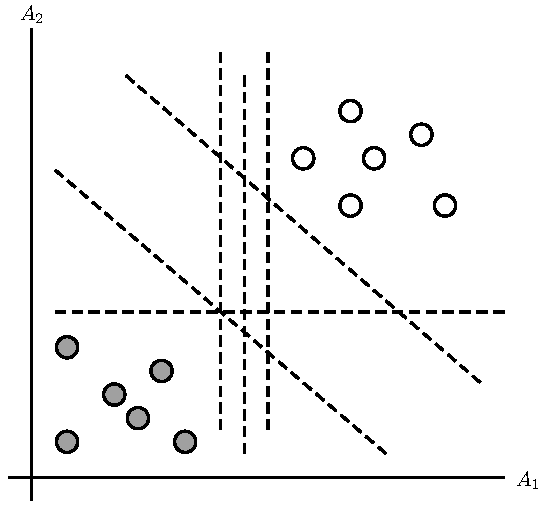
\includegraphics[width=0.6\textwidth]{svm2}
    %\caption[Example of linearly separable training data]
    %{Example of linearly separable training data in a two dimensional
    %space. There are an infinite number of (possible) separating hyperplanes or
    %\qt{decision boundaries} \cite[p. 338]{han2006data}.}
    %\label{fig:svm}
  %\end{center}
%\end{figure}

%SVMs are widely used nowadays, and have been successfully applied in areas such
%handwritten digit recognition, object recognition, and speaker identification,
%as well as benchmark time-series prediction tests \cite{han2006data}. They are
%typically regarded. They are highly accurate, due in part to their ability to
%model complex nonlinear decision boundaries.

%However, even the fastest SVMs can be extremely slow in both the training and
%testing steps. It is also directly limited to two-class tasks, requiring the use
%of other algorithms to reduce multi-class tasks to binary ones.

%\subsubsection*{K-NN}

%K-NN is a non-parametric method for classification and regression problems.
%First described in the early 1950s \cite{han2006data}, it is one of the simplest
%machine learning algorithms and is widely used in the area of pattern
%recognition.

%Nearest neighbor classifiers are based on the premise of learning by analogy, in
%other words, by comparing a given test tuple with similar training tuples. This
%classification of tuples as \qt{similar} is typically based on simple rules,
%like the \textit{Euclidean distance} between tuples.

%In k-NN, each training tuple is described by $n$ attributes and is represented
%as a point in an $n$-dimensional space. For classification problems, the test
%tuple is represented in this space, along with the training tuples. The unknown
%tuple is then assigned to the most common class among its $k$ nearest neighbors.

%K-NN as several advantages when compared to other classification algorithms. For
%one it has a very simple implementation. it is also very robust in terms of
%search space (the classes don't have to be linearly separable) and has few
%parameters, making it easy to tune. On the other side, it is an expensive method
%in terms of testing, as we need to calculate the distance between a testing
%tuple and every other known tuple. Furthermore, it is sensitive to noisy or
%irrelevant attributes and unbalanced datasets.

\subsubsection*{Inductive Logic Programming}

\begin{Notes}
- Still seems relevant, later refer that it wasn't possible to conduct ILP
clustering due to lack of time/problems with tools.\\
\end{Notes}

ILP is a subfield of machine learning that uses first order logic to represent
both data and models \cite{Lavrac1998}. ILP induces hypotheses (models) from
examples and background knowledge. Examples are of two types: instances of the
concept to be \qt{learned} and non-instances of the concept. Background
knowledge is a set of predicates encoding all information that the experts find
useful to construct the models. ILP might be used to tackle several machine
learning and data mining problems, like classification, regression and
clustering.

The first and most important motivation for ILP systems is that they overcome
the representation limitations of attribute-value learning systems, such as the
previously mentioned data mining algorithms. Attribute-value systems base their
representations of data in table based representations. Although effective in
many situations, these representation is not very expressive and might not even
be feasible for certain problems \cite{Bratko:1995:AIL:219717.219771}. The
second motivation for ILP is that by using a logical representation, the
hypotheses are understandable and interpretable by humans, being therefore
useful to explain the phenomenons that produce the data. This representation
also means that background knowledge can be represented and employed in the
induction process, in contrast to attribute-value models, where this information
is difficult to represent.

Despite these advantages, ILP cannot be applied indiscriminately to any
classification or regression problem. ILP systems are typically very heavy when
it comes to computational resource consumption and run for long periods of time
\cite{fonseca2003implementation}.

\subsection{Model Evaluation Procedures and Measures}\label{sec:mineval}

\begin{Notes}
- No longer relevant.\\
- Explain internal and external evaluation.\\
- Explain that due to the novelty of our analysis we will merely focus on
internal analysis.\\
- Describe some internal analysis measures (don't forget silhouettes).\\
\end{Notes}

%Creating a data model using a suitable classification algorithms is not the last
%step in the data mining process. At this point our model works well with the
%original training data, but we need to verify its power to generalize to other
%sets of data. Without this evaluation process, our models may be susceptible to
%problems like overfitting, in which the model wrongly describes a random error
%or data noise as a significant pattern \cite{han2006data}. As such, we need
%methods that allow us to test our models before deployment, as well as standard
%measures, to determine their quality.

%\subsubsection*{Evaluation Procedures}

%As stated, evaluation procedures are essential to verify the generalization
%capabilities of a given model. These procedures typically consist of dividing
%the test dataset in two or more subsets, using some of them for training and the
%others for testing. We will present a brief overview of some of these procedures
%below.

%\paragraph{Hold-Out}

%The \textit{hold-out} method reserves a part of the dataset for training
%purposes and uses the remaining data for testing \cite{witten2011data}.
%Typically we separate one third of the original dataset for testing, using the
%other two thirds for training.

%However, this arbitrary division of the dataset might be problematic if the
%subsets aren't representative of the population. For example, if the test subset
%is missing a class our results might be erratic. One way to attenuate this
%problem is to use stratification. Using stratification of the dataset we ensure
%that both subsets are representative, with approximately equal proportions for
%each class. We can lessen error rates even further and make the
%\textit{hold-out} estimate more reliable using the \textit{repeated hold-out}
%method. This is an iterative method, where in each iteration a subset is
%randomly selected to use as training (possibly using set stratification), using
%the remaining subset for testing. After all the iterations, the error rates of
%each one are averaged to yield an overall error rate.

%\paragraph{Cross-Validation}

%\textit{Repeated hold-out} methods pose a problem: the different test subsets
%will eventually overlap. This may cause that some examples never appear in the
%training subsets. The overlapping problem can be solved using the
%\textit{cross-validation} procedure, also called \textit{k-fold
%cross-validation}. This method consists in splitting the original dataset into
%\textit{k} subsets, using each subset in turn for testing and the remainder for
%training.

%The standard method for evaluation is \textit{10-fold cross validation}, where
%the dataset is divided into ten subsets. The subsets are typically stratified to
%reduce result variance. In each iteration one of the ten folds is picked as test
%and the other nine are used for training. Sometimes, to further reduce variance,
%\textit{repeated stratified cross-validation} is used, repeating normal
%\textit{10-fold cross-validation} ten times, then averaging the results.

%\paragraph{Leave-One-Out}

%\textit{Leave-one-out} method is a form of \textit{cross-validation}, taken to
%extreme lengths. In this particular method, the original dataset is divided into
%\textit{n} folds, where \textit{n} is the number is the number of individual
%training instances. It has some benefits, like allowing for a better use of the
%dataset and involving no random set sampling. However, the sheer number of folds
%and tests makes it a very computationally expensive method. Another disadvantage
%is that no stratification is possible, as there is always only one instance in
%the test subset.

%\subsubsection*{Common Measures}

%Applying evaluation procedures is not sufficient by itself. In order to appraise
%the quality of our models, we need to use standard quality measures, that give
%meaning to the obtained results. Below we will review some common measures, used
%in the context of classification problems.

%\paragraph{Precision}

%Precision determines the fraction of positive cases that are correctly
%identified as such. Low precision values mean that the model identifies many
%cases as positive when they are in reality false positives. Precision is
%calculated as shown in Equation \ref{eq:precision}.

%\begin{equation}
  %Precision=\frac{\tp}{\tp + \fp}
  %\label{eq:precision}
%\end{equation}

%\paragraph{Recall}

%Recall represents the portion of actual positive results in the dataset that
%were identified as such. From a statistical standpoint, it can be viewed as the
%average probability of find all the positive cases in the dataset. The value is
%computed using Equation \ref{eq:recall}.

%\begin{equation}
  %Recall=\frac{\tp}{\tp + \fn}
  %\label{eq:recall}
%\end{equation}

%\paragraph{Accuracy}

%Accuracy represents the percentage of predictions that are in fact correct. This
%measure relates to the ability of our model to correctly predict the class of
%new data. It can be calculated with Equation \ref{eq:accuracy}. For a given
%problem, better accuracy might not always mean that a model is better than
%another. As such, other measures like precision and recall are also taken into
%account.

%\begin{equation}
  %Accuracy=\frac{\tp + \tn}{\tp + \fp + \tn + \fn}
  %\label{eq:accuracy}
%\end{equation}

%\paragraph{F-Measure}

%F-measure is the harmonic mean of precision and recall. The reason behind the
%usage of an harmonic mean instead of an arithmetic mean is that the first is
%more intuitive, when computing a mean of ratios \cite{Sasaki2007}. F-measure is
%calculated as shown in Equation \ref{eq:fmeasure}. It is particularly useful to
%differentiate between cases where one of the variables (precision or recall) has
%a very high value and the other has a very low value. For example, if in a
%particular situation we have a precision of $1.0$ and a recall of $0.2$, the
%arithmetic mean would be $0.6$. However, a system with a recall as low as $0.2$
%might not be very useful. On the other hand, in the same situation the harmonic
%mean would be $0.333(3)$, giving a much more realistic measure of the quality of
%the model.

%\begin{equation}
  %\textit{F-measure}=2 \cdot \frac{\mathit{Precision} \cdot
  %\mathit{Recall}}{\mathit{Precision}+\mathit{Recall}} \label{eq:fmeasure}
%\end{equation}

%\paragraph{AUC}

%Sometimes in order to evaluate the quality of a certain model we might plot a
%ROC (or \textit{receiver operating characteristic}) curve. ROC curves depict the
%performance of a classifier without regard to class distribution or error
%costs. The curve is build by plotting false positive rates in the $x$ axis and
%true positive rates (recalls) in the $y$ axis (Figure \ref{fig:roccurve}).

%\begin{figure}[ht]
  %\begin{center}
    %\begin{tikzpicture}
      %\begin{axis}[
        %domain=0:1,
        %legend pos=south east,
        %xlabel=False Positive Rate,
        %ylabel=True Positive Rate]
        %\addplot[mark=none, samples=10, red] function {x};
        %\addplot[smooth, color=blue, mark=none]
          %plot coordinates {
              %(0.0,0.0)
              %(0.1,0.4)
              %(0.2,0.7)
              %(0.3,0.8)
              %(0.4,0.85)
              %(0.5,0.88)
              %(0.6,0.91)
              %(0.7,0.94)
              %(0.8,0.97)
              %(0.9,0.99)
              %(1.0,1.0)
          %};
        %\legend{Random model,Created model}
      %\end{axis}
    %\end{tikzpicture}
    %\caption[Example of ROC curve]{Example of ROC curve.}
    %\label{fig:roccurve}
  %\end{center}
%\end{figure}

%However, the curve can be hard to interpret at times. In this situation we can
%use the AUC measure (or \textit{area under the curve}), in order to condensate
%the curve's information in a single value. The AUC of a random classification
%system is $0.5$. This means that any model that as an AUC of $0.5$ is not able
%to distinguish between two groups. As the AUC increases, the model's quality
%also increases and at a value of AUC equal to $1.0$ the model is able to
%perfectly separate both groups.

\subsection{Data Mining Tools}\label{sec:mintools}

Except in rare cases of very specific problems, it typically makes no sense for
someone to implement any data mining algorithm that they might need. In fact,
today we have lots of data mining tools (many of which are free), that already
implement many of those algorithms. These tools are usually customizable, making
it easy to adapt them to most problems. Below we'll briefly review some of the
most popular data mining tools, that apply to the specific needs of this thesis.

\subsubsection*{RapidMiner}

\begin{Notes}
- Still relevant.\\
- Refer that RapidMiner and Weka were only used for testing purposes, and are
note part of the final solutions.\\
- Refer other relevant R packages.\\
\end{Notes}

RapidMiner\footnote{\url{http://www.rapidminer.com/}} is a complete solution for
data mining problems. it is available as a standalone GUI based application, as
seen in Figure \ref{fig:rapidminer}. It is a commercial application, although
its core and earlier versions are distributed under an open source license and
it offers a free version, beyond its multiple paid versions. Being one of the
most popular data mining tools used today, its applications span several
domains, including education, training, industrial and personal applications,
among others. Its functionality can also be easily extended through the use of
plugins\footnote{Plugin is a software module that adds new functionality to an
existing software application. Plugins are typically dependent on the platform
they extend and can't be used as standalone tools.}, reflecting in an increased
value for this tool. One such example in the area of bioinformatics is the
integration plugin between RapidMiner and the
Taverna\footnote{\url{http://www.taverna.org.uk/}} open source workflow
management system \cite{Jupp2011}.

\begin{figure}[!htb]
  \begin{center}
    \leavevmode
    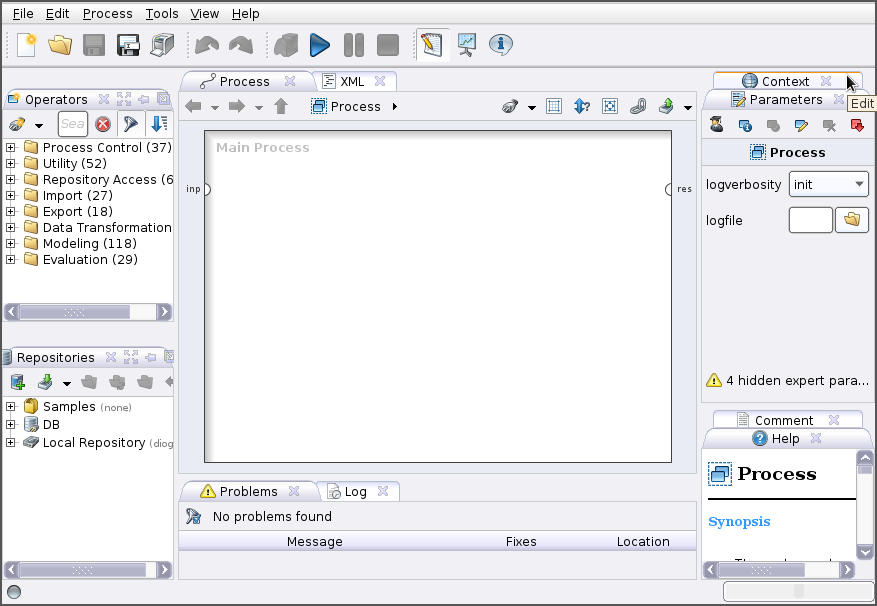
\includegraphics[width=1.0\textwidth]{rapidminer}
    \caption[RapidMiner user interface]{RapidMiner user interface.}
    \label{fig:rapidminer}
  \end{center}
\end{figure}

\subsubsection*{Weka}

Weka\footnote{\url{http://www.cs.waikato.ac.nz/ml/weka/}} is an open source tool that
collects several machine learning algorithms and allows its user to easily apply
those algorithms to data mining tasks \cite{Hall}. Created at the University of
Waikato, New Zeland in 1997 (the current version was completely rewritten in
1997, despite the first iteration of the tool being developed as early as 1993),
it is still in active development to date. Weka supports several common data
mining tasks, like data preprocessing, classification, clustering, regression
and data visualization. it is core libraries are written in Java and allow for an
easy integration of its data mining algorithms in pre existing code and
applications. Other than that, Weka can be used directly through a command
line/terminal or through one of its multiple GUIs (Figure \ref{fig:weka}). Its
simple API and well structure architecture allow it to be easily extended by
users, should they need new functionalities.

\begin{figure}[!htb]
  \begin{center}
    \leavevmode
    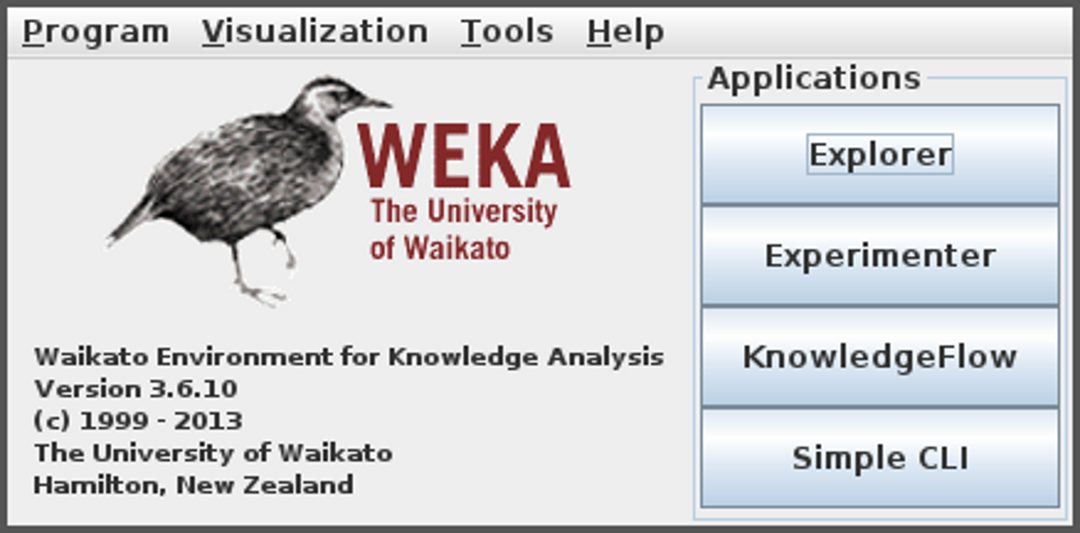
\includegraphics[width=0.7\textwidth]{weka}
    \caption[Weka interface selection]{Weka interface selection.}
    \label{fig:weka}
  \end{center}
\end{figure}

\subsubsection*{R Language}

R\footnote{\url{http://www.r-project.org/}} is a free programming language and
software environment for statistical computing and graphics generation.
Originally developed by Ross Ihaka and Robert Gentleman at the University of
Auckland, New Zealand in 1993 \cite{Ihaka1998}, it is still under active
development. R is typically used by statisticians and data miners, either for
direct data analysis or for developing new statistical software \cite{Fox2005}.

R is an implementation of the S programming language\footnote{S is an object
oriented statistical programming language, appearing in 1976 at Bell
Laboratories.}, borrowing some characteristics from the Scheme programming
language. it is core is written in a combination of C, Fortran and R itself. It
is possible directly manipulate R objects in languages like C, C++ and Java. R
can be used directly through the command line or through several third party
graphical user interfaces like
Deducer\footnote{\url{http://www.deducer.org/pmwiki/index.php}}. There are also
R wrappers for several scripting languages.

R provides several different statistical and graphical techniques, including
linear and nonlinear modeling, classical statistical tests, time-series
analysis, classification, clustering, among others. It can also be used to
produce publication-quality static graphics. Tools like Sweave
\cite{lmucs-papers:Leisch:2002} allow users to embed R code in \LaTeX{}
documents, for complete data analysis.

\paragraph{Bioconductor Package}

Bioconductor is a free and open source set of tools for genomic data analysis,
in the context of molecular biology \cite{lmucs-papers:Leisch:2002}. It is
primarily based on R. It is under active development, with two stable releases
each year. Counting with more than seven hundred different packages, it is the
most comprehensive set of genomic data analysis tools available for the R
programming language. It also provides a set of tools to read and manipulate
several of the most common file formats used in molecular biology oriented
applications, including FASTA, FASTQ, BAM and GFF.

\section{Chapter Conclusions}

\begin{Notes}
- Remove the uncertainty part, talk about what was done.\\
\end{Notes}

In this chapter we gave a brief introduction of the molecular biology concepts
that serve as base of the thesis. We also reviewed the concepts on RNA-Seq and
data mining and presented short analyses of concrete tools that will likely be
used during the project.

At this moment we do not possess all the necessary information about the dataset
that will be used in the data mining phase of the project. We are unable, at the
present, to determine the nature of our data, which means that we cannot predict
whether it could be modeled by classification algorithms. As such, we presented
ILP as an alternative approach for this situation. In case ILP techniques become
in fact necessary, further work will include a more profound and complete
revision.

\chapter{Solution Description} \label{chap:description}

\section*{}

In this chapter we present the designed solution. The main objectives of the
solution's design are reviewed, along with the most important choices made. Both
major components of the developed solution and their envisioned integration
process are described in detail.

\section{Overview}

%\begin{Notes}
%- Problem divided into two subproblems.\\
%- Both problems solvable independently.\\
%- Availability, scalability, etc.\\
%\end{Notes}

As discussed, from a purely biological standpoint, this thesis has two major
objectives: to perform differential expression analysis of RNA-Seq data and to
discover and characterize RBPs related to groups of genes. While both objectives
are important for our particular domain problem, they present different problems
and require different approaches. Furthermore, both parts of the problem are
relevant by themselves.

Splitting the domain problem into two objectives led to the first important
design decision. It was decided that the software solutions to both problems
would be implemented independently and, at a later stage, integrated with each
other, to form the complete system. This would also allow both tools to be used
separately, leading to a wider array of possibilities in terms of future uses.

Designing software solutions with high performance, scalability and
extensibility is also a major concern. A software solution should be able to
quickly and efficiently fulfil a user's requests, while dealing with a large
number of simultaneous users. It should allow new features to be easily added,
in order to better respond to the users' needs. If these requirements are not
met, the solution is at risk of being abandoned by its users, becoming therefore
useless. The software solutions presented in this thesis were designed with
these goals in mind, as is further discussed in Chapter
\ref{chap:implementation}.

\section{Gene Expression Analysis Pipeline}

%\begin{Notes}
%- Uses iRAP as a base pipeline.\\
%- Show analysis workflow (diagram).\\
%- Simple graphical configuration with best settings inferring and advanced
%mode.\\
%- Standard data always available, with possibility of user upload.\\
%- User data sent by link or direct upload.\\
%- Results from different differential expression tools are combined.\\
%\end{Notes}

The gene expression analysis pipeline uses iRAP \cite{irap} as its foundation.
As discussed before, iRAP provides begin-to-end gene RNA-Seq data analysis.
However, while iRAP is a tool aimed at a broad group of users, both beginners
and advanced users, it is still a command line tool, with many configuration
settings. This technological barrier may drive away some more inexperienced
users. One of the objectives of this part of the work was to make it a simpler
and more straightforward process, accessible to any user with basic computer
literacy; another was to combine results of several different tools, with the
aim of improving those results. Note that some of the features described below
were not implemented, due to time constraints. As such, those features are
presented as future work.

\subsection{Analysis Configuration}

iRAP is configured with an experience configuration file (see Appendix
\ref{appendix:irapconfig}). This file must define the name of the species being
analysed, the reference and read data files, the tools to use for the analysis,
read libraries, etc.. Although many of these configurations are difficult to
infer and define automatically, it is possible to create a more user friendly
way to configure the experiments. This is accomplished through a web form. This
web form has two different views: the \emph{normal view} allows users to
configure only the essential settings of the experiment, those that cannot be
inferred; the \emph{advanced view} allows more experienced users to tweak every
configuration.

\subsection{Experimental Data Management}

Gene expression analysis with iRAP requires two sets of files, \emph{reference
files} and \emph{read data files}.

Reference files are both the reference genome (in FASTA format) and its
annotations (in GTF or GFF formats). These files are automatically obtained from
Ensembl's FTP endpoint. The current release contains information of a total of
sixty six species. The tool automatically checks if a new release is available,
and in that case downloads and substitutes the files. In the experiment
configuration users need only to indicate which species they are analysing, and
the correct files will be automatically passed to iRAP.

Read data files contain the reads obtained through sequencing, in FASTQ formats.
The user needs to upload these files. One file must be provided for each library
the user wants to analyse, and should be compressed. As some of these files can
be quite large, users also have the possibility to provide a link to those
files. If a link is provided, the files will be downloaded before the analysis
starts.

\subsection{Analysis Workflow}\label{sec:descworkflow}

Once both the configuration file and the required data files are ready, the
analysis process can begin. The analysis process starts by passing those files
to iRAP (Figure \ref{fig:tool1}). In this initial stage of the workflow the
analysis will stop immediately after the quantification step (see Section
\ref{sec:irap}).

\begin{figure}[!htb]
  \begin{center}
    \leavevmode
    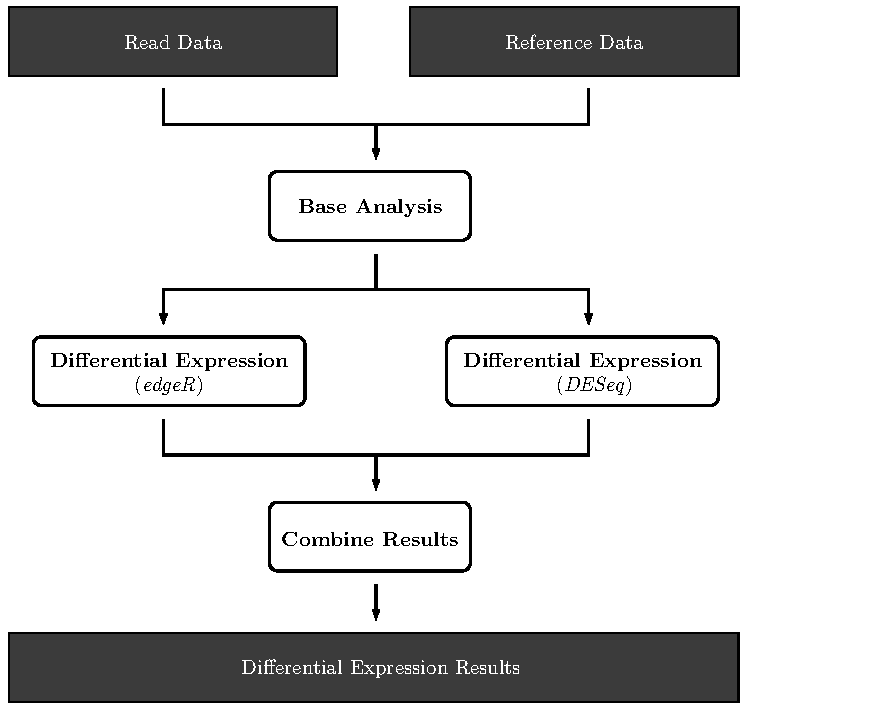
\includegraphics[]{tool1}
    \caption[Gene expression analysis pipeline workflow]{
      Gene expression analysis pipeline workflow.
    }
    \label{fig:tool1}
  \end{center}
\end{figure}

The next step is to sequentially execute differential expression analysis with
the chosen tools, in this case DESeq \cite{20979621} and edgeR
\cite{robinson2010edger}. The resulting files are kept until all tools are
executed. Note that there is no need for the analysis process to start from the
beginning every time a new tool is used, as iRAP can (in most cases) reuse the
results produced up until the point where a new tool is introduced.

After all tools are executed their results must be combined into a final list of
gene identifiers. This is done in an attempt to give researchers an higher level
of confidence in differential expression results. Note that this process is not
part of the iRAP analysis pipeline, and therefore a new tool must be developed.
Algorithm \ref{algo:combine} shows the basic process of combining the obtained
differential expression results. First, entries in every file must be filtered
by their \emph{p-value}\footnote{A \emph{p-value} is used to assert the
statistical significance of results. It represents the probability of obtaining
the same as before in a new sample, given that the null hypothesis is true
\cite{goodman45dirty}.}, that must be inferior to a maximum threshold ($0.05$ by
default). Then all entries in all files are compared with each other. This
produces an intersection of all files, in other words, a list of entries that
are present in all files.

\begin{algorithm}
  \emph{genes} = empty map\;
  \emph{files} = load all result files\;
  \ForEach{file \emph{in} files}{
    \ForEach{entry \emph{in} file}{
      \If{entry.pvalue $\leq$ 0.05}{
        increase gene count in \emph{genes}[\emph{entry.gene}]\;
      }
    }
  }
  \ForEach{gene, count \emph{in} genes}{
    \If{count $<$ number of files}{
      remove \emph{gene} from \emph{genes}
    }
  }
  write \emph{genes} to a file\;
  \BlankLine

  \caption[Combination of differential expression results]{
    Combination of differential expression results.
  }
  \label{algo:combine}
\end{algorithm}

\section{RNA Binding Protein Analysis Web Platform}

%\begin{Notes}
%- Present the name!\\
%- Minimal user input, infer most information.\\
%- Show analysis workflow (diagram).\\
%- Present standard RBP information.\\
%- Data set enrichment: show transcripts, proteins and their information
%(describe all info).\\
%- Two different types of clustering analysis, based on the used data and
%clustering criteria (describe algorithms, selection, etc.).\\
%- Briefly describe ERDA ILP analysis (and say it failed).\\
%\end{Notes}

The main objective of this system is to transform a complex, manually performed
analysis, into an automated workflow. The platform should require as little
information as possible from the user, inferring analysis parameters whenever
possible. It should also be able to automatically group genes (and proteins), to
reveal implied relationships between them that might be useful to experts. This
platform was named Protein Binding Site Finder (PBS Finder) and shall henceforth
be referred to by that name.

\subsection{Experimental Data}

The only data PBS Finder collects from the user is a list of gene (or
transcript) identifiers that should be analysed. These identifiers can be in one
of five different formats: \emph{Ensembl Gene}, \emph{Ensembl Transcript},
\emph{Entrez}, \emph{RefSeq} or \emph{GenBank} ( see Table \ref{tab:examples}).
Users can submit jobs with any combination of the previous types and use
identifiers from multiple species.

\begin{table}[!htb]
  \centering
  \begin{tabular}{{l} | {l}{l}}
    \textbf{\emph{Ensembl Gene}}        & ENSG00000224274 & ENSRNOG00000013536\\
    \textbf{\emph{Ensembl Transcript}}  & ENST00000003156 & ENSRNOT00000117589\\
    \textbf{\emph{Entrez}}              & 11245           & 66850\\
    \textbf{\emph{RefSeq}}              & NM\_001107622.1 & NM\_031098.1\\
    \textbf{\emph{GenBank}}             & U49845          & C35522\\
  \end{tabular}

  \caption[Examples of identifiers accepted by PBS Finder] {
    Two sets of examples of identifiers accepted by PBS Finder.
  }
  \label{tab:examples}
\end{table}

While PBS Finder can accept all these kinds of identifiers, internally the
analysis can only be started with \emph{Ensembl Gene} or \emph{Entrez}
identifiers, that map to Ensembl's and NCBI's pages, respectively. As such, the
identifiers must be first separated into different groups and converted. This
conversion is reviewed with more detail in Section \ref{sec:pbsworkflow}.

\subsection{User Information Management}

In order to use PBS Finder a new user must create an account, providing their
name and email, and choosing their authentication password. The account system
was implemented so that jobs could be associated with their creator in a cross
browser/system manner, in contrast with a typical cookie-based\footnote{Modern
websites sometimes need to save information about the user, for example
credentials. This data can be saved in the client machine, through the use of a
web browser cookie.} data persistence. This allows each user to list their own
jobs. Despite jobs being only directly accessible by their owner (creator), no
effort was made to deny users access to each other's jobs through the job's URL.
We believe that sharing results is an essential part of the investigation
process.

To create a new job the user provides a job description and an identifier list.
The identifier list is a newline-separated list (a single entry per line) of
unique identifiers for genetic information databases. In the current version
acceptable types of identifiers include Ensembl (both Gene and Transcript),
Entrez, RefSeq and GenBank. Users can submit jobs with any combination of the
previous types and use identifiers from multiple species. Upon job creation,
users can choose to be notified by email when the job finishes.

\subsection{Analysis Workflow}\label{sec:pbsworkflow}

PBS Finder is based around a three stage analysis model (Figure
\ref{fig:workflow2}): \emph{base analysis}, \emph{data set enrichment} and
\emph{clustering analysis}.

\begin{figure}[!htb]
  \begin{center}
    \leavevmode
    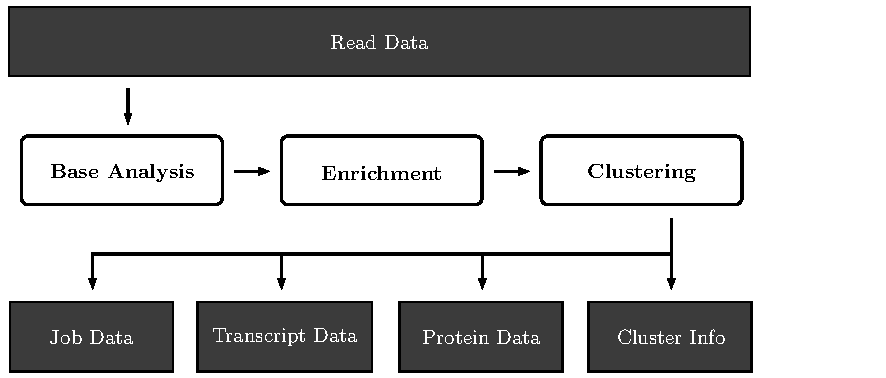
\includegraphics[width=0.75\textwidth]{workflow2}
    \caption[Simplified PBS Finder workflow]{
      Simplified PBS Finder workflow.
    }
    \label{fig:workflow2}
  \end{center}
\end{figure}

Base analysis comprises data set filtering, retrieval of basic gene and
transcript information and finding RBPs. The first released version of the
platform implemented only this stage of the analysis. It contains all the
information that is necessary to answer one of the base thesis problems.
However, further stages build on top of this information, bringing a more
valuable set of results to biologists.

In the enrichment stage additional information about every protein is retrieved.
This information is obtained from
UniProt\footnote{\url{http://www.uniprot.org}}, a web platform for curated
protein information. This stage was implemented in the second release of the
platform.

The clustering stage takes all the information collected in the previous stages
and uses it to perform clustering analysis. There are two types of clustering
analysis performed: \emph{clustering using RBP presence} and \emph{clustering
using RBP attributes}. The objective of this analysis is to uncover implicit
relationships in the collected data, that may be of use to biologists.

These stages are described in more detail in Chapter \ref{chap:implementation}.

\section{Tool Integration}

%\begin{Notes}
%- Complex pipeline with both tools.\\
%- Result reporting at each component.\\
%- Combined result reporting at the end.\\
%- Show integration diagram.\\
%\end{Notes}

In the designed solution both tools should be able to integrate, so that a user
could perform the complete analysis creating a unique analysis job. This would
be accomplished by using the interface of the RNA-Seq analysis pipeline as the
master (or main) interface for job creation. When the analysis completes, the
pipeline presents the preliminary results to the user and automatically launches
a PBS Finder analysis for the result gene identifier list. At this point the
RNA-Seq pipeline's interface should include a direct link to the created job in
PBS Finder. That link can then be used by the user to view the results of the
RBP localization analysis. Note that, while both tools are now integrated, the
results of both analyses are independent. As such, they can be
consulted/reviewed independently from each other, as if both had run separately.

\section{Chapter Conclusions}

%\begin{Notes}
%- Generic chapter conclusion.\\
%- Introduce next chapter of implementation details.\\
%\end{Notes}

In this chapter we reviewed the most important details about the design of the
proposed software solution (implementation details are described in Chapter
\ref{chap:implementation}). We presented the modular, two subsystem model, that
allows both tools to be used as standalone products, increasing the number of
their possible uses. Lastly, we talked about the general details of the
workflows of both tools, as well as the integration of those workflows.

\chapter{Implementation} \label{chap:implementation}

\section*{}

In this chapter we present and discuss some specific details of the
implementation of the designed solution. We will also review some of the used
technologies, and provide the rational behind their choice, whenever relevant.

%\begin{Notes}
%- Talk about iRAP configuration, the result combination tool and more.\\
%- Talk about PBS Finder configuration, requisites and analysis flow (show that analysis flow diagram).\\
%- Talk about platform extensibility, deployment alternatives and more.\\
%\end{Notes}

\section{Gene Expression Analysis Pipeline}

%\begin{Notes}
%- Describe platforms and minimum requirements.\\
%- Describe iRAP deployment.\\
%- Describe result combinator usage.\\
%\end{Notes}

Due to time constraints the gene expression analysis pipeline could not be fully
finished. Integration with PBS Finder's analysis pipeline was not accomplished.
Similarly, it was also not possible to provide the RNA-Seq analysis pipeline's
functionality through the web interface. However, both the iRAP pipeline and the
results combining program were completed and functional.

\subsection{Combining Differential Expression Results}

The results combining tool was implemented in the form of a Ruby script. As a
command line script this tool can be easily integrated with the existing iRAP
workflow, as iRAP is also completely executed in the command line.

The results of differential expression produced by iRAP are exported as
\emph{tab-separated values} (TSV) files. Each differential expression analysis
tool produces a TSV file for each contrast that is analysed. These files contain
gene identifiers and a variety of statistical values for each identifier,
including the \emph{p-value}.

The tool takes all files from a single contrast, filters entries by
\emph{p-value} and counts the number of times each gene identifier is found.
Note that each file has at most one occurrence of a gene identifier. Every
identifier that appears in all files is exported to the text file that contains
the combined results. This file can then be used as input for the RBP analysis
platform, obtaining further information about those genes.

An example of the use of this module is provided in Section
\ref{sec:irap_comparison} of Chapter \ref{chap:casestudy}

\section{RNA Binding Protein Analysis Web Platform}

%\subsection{Application Architecture}

%\begin{Notes}
%- Client-server architecture.\\
%- Web app is responsible for user and job management, viewing information, etc.
%(uses Padrino + MongoDB).\\
%- Worker server is responsible for analysis.\\
%- Server uses DRb, spawns a new thread for every analysis request it receives
%(show algorithm).\\
%- Server is agnostic to the analyser being executed, it just dynamically
%instantiates a analyser requested by the web app.\\
%\end{Notes}

PBS Finder is implemented in two parts, following a client-server architecture:
the \emph{web interface} and the \emph{analysis server}. In this case the web
interface is the client and the analysis server is the server. This means that,
whenever a user submits an analysis job, the web interface sends an analysis
request to the server, including the data set given by the user. The server then
processes the request and reports the results back to the web interface, that
presents them to the user.

\subsection{Web Interface}

PBS Finder's web application interface is written in Ruby, using the
Padrino\footnote{\url{http://www.padrinorb.com}} framework. Padrino is a web
framework built on top of the Sinatra\footnote{\url{http://www.sinatrarb.com}}
web library. Padrino allows the creation of web applications that use Ruby to
define their back-office logic.

\subsection{Data Persistance}

User and job data is persisted in a database; in this case the
MongoDB\footnote{\url{http://www.mongodb.org}} database system was chosen.
MongoDB is a document based, NoSQL database. While widely adopted relational
database management systems rely on large data banks and relational calculus,
NoSQL databases store information in the form of documents
\cite{strauch2011nosql}, instead of relational table records. NoSQL databases
sacrifice the possibility to use some complex mechanisms of classical relational
databases (for example structured queries and enforced information integrity),
in order to achieve higher performance and scalability. NoSQL databases are most
effective when the saved records are large but are seen as loosely structured
collections of information.

\subsection{Analysis Server}

The analysis server is responsible for managing analysis requests sent by the
web interface. The server is implemented on top of Distributed Ruby (dRuby), a
distributed object system for Ruby. dRuby allows methods and behaviours to be
invoked on an object that exists in a different process or even in a different
computer, using a network connection. From the client's point of view it seems
like the object is local, as it can be used as any other object. The server uses
a master distributed object to receive analysis requests from the web interface.

The server launches each job concurrently. This behaviour allows the server to
run multiple analyses at the same time. Note that the server is not bound to a
single type of analysis, it can perform any type of analysis, as long as a valid
implementation is available. The only two constraints to create a new type of
analysis are that the analysis workflow must be encapsulated inside an
instantiable class. That class must implement a defined interface, in other
words, it must implement a simple set of methods that allows the server to
control it. As such, new analysis methods can be easily added in the future as
their core functionality can be opaque to the server as long as they implement
the server's interface.

Algorithm \ref{algo:server} represents the behaviour of the server when a new
request arrives. The first step is to determine if the requested analysis method
is available. If it is, the corresponding class is instantiated, and the
analysis data set (and other relevant information) is passed to it. Note that
at the same time the server creates a file with a copy of all the parameters of
that particular request. If for some reason the server stops working, analyses
that were running at that time will be automatically restarted once the server
is available again. After the object that will be responsible for the analysis
is created, the server creates and starts a new thread for it. The server also
saves an indication that that particular analysis is being executed.

\begin{algorithm}
  receive request\;
  \uIf{request.analysis\_method \emph{is available}}{
    instantiate \emph{request.analysis\_method} with \emph{request.parameters}\;
    save \emph{request.parameters} to disk\;
    run the analysis in a new thread\;
    \uIf{success}{
      report results\;
    }
    \Else{
     report error\;
    }
    delete \emph{request.parameters} from disk\;
  }
  \Else {
    report error\;
  }
  \BlankLine

  \caption[Processing a new analysis request from the web interface]{
    Processing a new analysis request from the web interface.
  }
  \label{algo:server}
\end{algorithm}

Once the analysis is complete the server is notified through its distributed
instance, and the results are communicated to the web interface. This also
prompts the server to eliminate both the indication of the running analysis from
its internal list and the file with the analysis' parameters from the file
system.

%\begin{Notes}
%- Configuration is based on external files.\\
%- While almost everything is configurable, only the clustering settings need to
%be messed with.\\
%\end{Notes}

\subsection{Analysis Workflow}

%\begin{Notes}
%- Present image.\\
%- Describe each part of the analysis and enrichment in detail, including used
%platforms.\\
%- Describe both types of clustering.\\
%- Describe the generation and application of all the clustering techniques.\\
%- Described how the best results are selected for each type of clustering (show
%algorithm).\\
%- Refer ILP and ERDA.\\
%- Tell how we couldn't get ERDA to work.\\
%\end{Notes}

A detailed overview of the RBP analysis workflow can be seen in Figure
\ref{fig:workflow}. This workflow is composed by three main stages: \emph{base
analysis}, \emph{data set enrichment} and \emph{clustering analysis}, all of
which will be described in detail below.

\begin{figure}[!htb]
  \begin{center}
    \leavevmode
    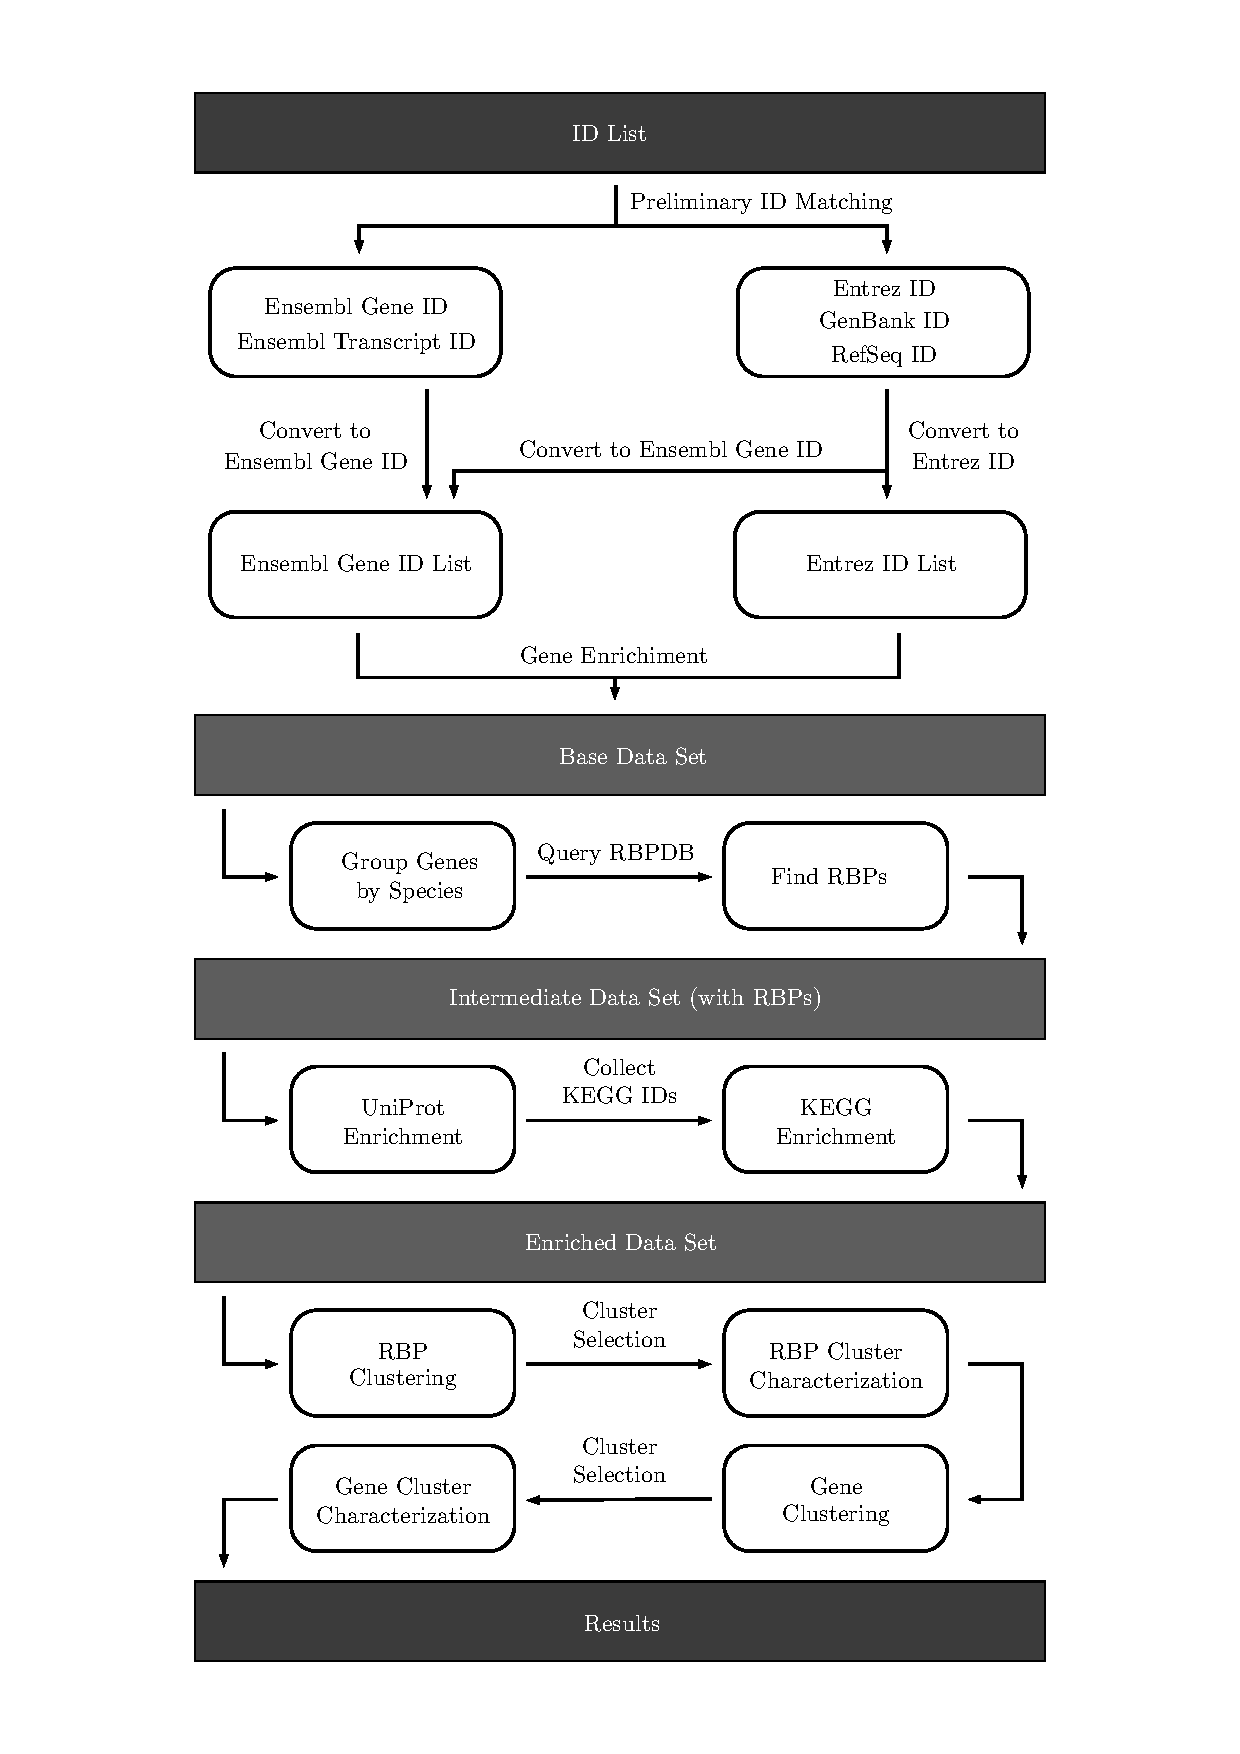
\includegraphics[width=0.73\textwidth]{workflow}
    \caption[PBS Finder workflow]{
      PBS Finder workflow. Note that error paths were not represented for
      simplicity. However, every component implements health checks, that may
      stop the entire analysis if the minimum requirements for success are not
      met.
    }
    \label{fig:workflow}
  \end{center}
\end{figure}

\subsection{Base Analysis}

The first step in the pipeline is to prepare the gene identifiers for the
following analysis steps. These identifiers can be written in five different
notations, as described in Section \ref{sec:descworkflow}. As such, identifiers
are separated according to their automatically detected notation in those five
groups. However, some of those identifiers may be invalid, despite appearing to
fit in one of the possible notations. It is assumed that if an identifier is
valid, it can at least be converted to either \emph{Ensembl Gene} or
\emph{Entrez} notation. These notations were chosen because they are the native
notations for genes in the used platforms (Ensembl and NCBI). This conversion is
done using bioDBnet's \cite{Mudunuri15022009} identifier conversion service. The
service was chosen for its simplicity and its large conversion database, that
draws from multiple conversion services like NCBI or Ensembl. \emph{Entrez}
conversion is only attempted if \emph{Ensembl Gene} conversion is not available.
While none of those platforms are preferred, converting as many identifiers as
possible to one convention helps to maintain data set coherence.

Since only two lists remain, one with \emph{Ensembl Gene} identifiers and the
other with \emph{Entrez} identifiers, information about those genes' transcripts
must be collected. This information includes the transcript's name, its
identifier, and its relevant genetic sequences. This information is collected
using their corresponding platform (Ensembl or NCBI).

The transcript sequences are then used to retrieve the related RBPs using RBPDB,
an online RNA binding protein database \cite{Cook01012011}. For each sequence
RBPDB finds every possible RBP, along with its name, location and binding
sequence. A complete list of all information retrieved for both genes and
transcripts can be found in Table \ref{tab:info_gene}. For a specific
transcript, if the retrieved 3’ UTR sequence is at least three hundred base
pairs long it will be used with RBPDB. If the 3’ UTR is too short, the 3’ UTR
downstream sequence (genomic sequence) will be used, with a fixed length of one
thousand base pairs. If none of the above situations is possible, the 3’ UTR
will be used as is (if it is at least one base pair long). Note that while the
5' UTR sequence is also collected (when available), the consulted experts were
interested in analysing only the 3' region. This information is sufficient to
answer one of this thesis' problems. However, it will be enriched and further
analysed, bringing greater benefits to researchers.

\begin{table}[!htb]
  \centering
  \caption[Information retrieved for genes and transcripts in the base analysis stage]{
    Information retrieved for genes and transcripts in the base analysis stage.
    Information marked with \qt{*} represent optional information; it might be
    relevant to the researcher and is therefore shown if available, but it is
    not crucial to the analysis. On the other hand, the unmarked fields
    represent required information, without which analysis on that particular
    gene/transcript cannot continue.
  }
  \label{tab:info_gene}

  \begin{tabular}{{l} | {l}}
    \multirow{3}{*}{\textbf{\emph{Gene}}}
    & Transcript identifiers\\
    & Gene name*\\
    & Species*\\ \hline
    \multirow{3}{*}{\textbf{\emph{Transcript}}}
    & Protein identifiers\\
    & Transcript name*\\
    & Genetic sequences (3' UTR, 3' UTR downstream, 5' UTR)\\
    & Names, locations and bind sequences of RBPs\\
  \end{tabular}

\end{table}

\subsection{Data Set Enrichment}

Given the RBP names obtained in the base analysis stage, a query is made to
UniProt in order to obtain their respective accession identifiers. These are
used internally by UniProt to refer to specific proteins. With the accession
identifiers, the pages for each RBPs can be retrieved and analyzed individually.
These pages contain information about their respective RBPs, including keywords,
related tissues and information about the RBPs' ontologies (cellular components,
molecular functions and biological processes).

The information collected from UniProt may also contains links to the KEGG web
platform. Among other useful information, KEGG contains information about
protein pathways. A pathway is a sequence of actions, related to specific
molecules, that produce certain changes within a cell, when performed. This
information is crucial to understand the function of RBPs. As such, it is
collected for further analysis (see Table \ref{tab:info_prot} for a complete
list of all information retrieved).

The first step for this phase is to use the protein names to retrieve a list of
matching \emph{UniProt Accession} identifiers. By default PBS Finder will try to
find a reviewed accession whose species matches the species in question. If this
is not possible it will fallback to an unreviewed accession, from the same
species. In case this is also not possible, it will try to find a reviewed human
analogue accession or, as a last case, an unreviewed one. After finding the
identifiers, the batch retrieval service is used to enrich the protein
information. This information includes ontologies, related tissues, and
references to external databases. From these references, KEGG identifiers in
particular are used to retrieve information about pathways in which the RBPs are
expressed. For each pathway, both its name and link to the KEGG pathway viewer
are provided.

\begin{table}[!htb]
  \centering
  \caption[Information retrieved for proteins in the data set enrichment stage]{
    Information retrieved for proteins in the data set enrichment stage.
    Information marked with \qt{*} represent optional information; it might be
    relevant to the researcher and is therefore shown if available, but it is
    not crucial to the analysis. On the other hand, the unmarked fields
    represent required information, without which analysis on that particular
    protein cannot continue.
  }
  \label{tab:info_prot}

  \begin{tabular}{{l} | {l}}
    \multirow{8}{*}{\textbf{\emph{Protein}}}
    & Protein name\\
    & UniProt identifier\\
    & Accession species\\
    & Related tissues*\\
    & Keywords*\\
    & Pathways*\\
    & Ontologies*\\
    & URLs to external platforms*\\
  \end{tabular}
\end{table}

\subsection{Clustering Analysis}

The last stage of the workflow is clustering analysis. Two different types of
clustering approaches were conceived: \emph{clustering by RBP presence} and
\emph{clustering by RBP information}. Note that this analysis will not be
performed if the quantity of available data is below certain thresholds
(typically the tool will not analyse data sets that have less than ten genes
and/or ten RBPs).

\subsubsection*{Clustering by RBP Presence}

In the first case, the clustering analysis is only conducted at the gene level.
Two genes are similar if they are associated with the same RBPs. Inversely, two
genes that do not have any (or few) RBPs in common are considered \qt{distant}. The
tool makes an additional step in order to determine which RBPs are common in one
particular group, while being absent in all the other groups. This information
allows researchers to easily determine which RBPs can be used to interact with a
particular group of genes, while not affecting the others.

\subsubsection*{Clustering by RBP Information}

In the second case the clustering process has two phases. In the first phase
RBPs are grouped based on their similarity. Similarity is computed using a set
of attributes that include (depending on availability): pathways; tissues where
the RBP is expressed; keywords describing their main functions; and other
relevant information such as ontologies (biological processes, molecular
function and cellular components). The tool compiles a list of defining features
for each group (to later present to the user). However, in this case the RBP
groups will be used to group similar genes. Unlike the previous method,
similarity between genes is not only measured in how many RBPs they have in
common. In this case any two genes may be considered similar if both are related
to RBPs that were grouped together in the previous step, even if they do not
share exactly the same RBPs between them.

\subsubsection*{Setup Variation}

To produce the final results multiple clustering experiments are attempted. Due
to the small amount of time that the chosen clustering algorithms need to run it
is possible to execute a large number of attempts and then choose only the best
results. Each attempt is a variation of the analysis parameters, being that each
possible value for a parameter is combined with every value for the remaining
parameters, giving rise to a large number of experiments. When clustering by RBP
presence the variable parameters are: clustering algorithm (either hierarchical
clustering or partitioning around medoids); and the number of clusters (between
two and ten). While clustering by RBP information the same variable attributes
apply. However, the decision about what RBP information is used for their
comparison is also variable, from a minimum of two information fields. For
example, in a particular clustering attempt only information about the RBPs'
pathways and related tissues may be used, while another attempt may use all
available information. Furthermore, for this particular type of analysis the
representation of the data set can also vary. The data set can be represented
either as a binary matrix (as is the case in clustering by RBP presence) or by a
Jaccard distance matrix, calculated from the sets of possible values for each of
the protein's attributes.

\subsubsection*{Result Selection}

With the large number of results obtained from all the clustering attempts, it
is not reasonable to expect a user to manually choose the ones that are most
interesting. As such, internal evaluation techniques for clustering are coupled
with rules that define minimum acceptance criteria for results, narrowing the
result space to only one for each type of clustering. Algorithm
\ref{algo:secsel} represents the method used for result selection.

\begin{algorithm}
  sort clustering results by average silhouette (descending)\;
  filter clustering results with clusters with less than 8\% of data set objects\;
  \emph{abundance\_frequency} = 0.90\;
  \While{abundance\_frequency $\geq$ 0.50}{
    \ForEach{clustering result}{
      classify as abundant any attribute with frequency $\geq$ \emph{abundance\_frequency}\;
      remove abundant attributes that appear in multiple clusters\;
      \uIf{at least one unique abundant attribute exists for each cluster}{
        select cluster\;
        break loop\;
      }
      \Else{
        \emph{abundance\_frequency} = \emph{abundance\_frequency} $-\ 0.05$\;
      }
    }
  }
  \uIf{a cluster was selected} {
    return selected cluster\;
  }
  \Else{
    return cluster with highest average silhouette\;
  }

  \caption[Selection of best clustering results]{
    Selection of best clustering results.
  }
  \label{algo:secsel}
\end{algorithm}

\subsubsection*{ILP Clustering}

Clustering using ILP techniques was also attempted. The main objective of this
approach was to uncover more information about the implicit relationships
present in the data sets. While conventional clustering methods present only the
data set objects grouped in clusters, with ILP it is possible to understand
exactly what rules were used to form those clusters.

The devised approach had two steps. First, the results for each new job would be
represented in the form of Prolog clauses. Second, those clauses would be used
as data set for the ERDA \cite{fonseca2012conceptual} clustering system, running
on top of YAP Prolog \cite{citeulike:8884858}. However, due to problems with the
available tools, this approach could not be included in the current version of
PBS Finder.

\subsection{Web Interface}

%\begin{Notes}
%- Talk about all information available in each view.\\
%- Talk about the types of results to export.\\
%- Talk about GridFS, and the need of pre generate results files to minimize long
%loading times.\\
%\end{Notes}

\subsubsection*{Job View}

Job view, also known as main view, is the default projection of a job's results
(Figure \ref{fig:job_view}). It gives the user a matrix that matches every gene
(and transcript) in the data set with their corresponding binding proteins, as
well as an histogram of the genes (a bar chart of the number of genes with which
each RBP binds). This matrix also contains two columns that provide information
about how the genes were grouped, based on the two distinct clustering
techniques. In addition to this information, clicking any group of genes will
give the user a list of all the characteristics that differentiate that
particular group from all the others.

This view also contains a mechanism that allows users to provide feedback and
report problems. Clicking the \qt{Report a problem} button the user is presented
with a form that allows them to provide a brief description of the problem. If
the user chooses to send that report, the web platform will send an email to its
administrator, containing the submitting user's information, the problem
description and a direct link to the offending page.

\begin{figure}[!htb]
  \begin{center}
    \leavevmode
    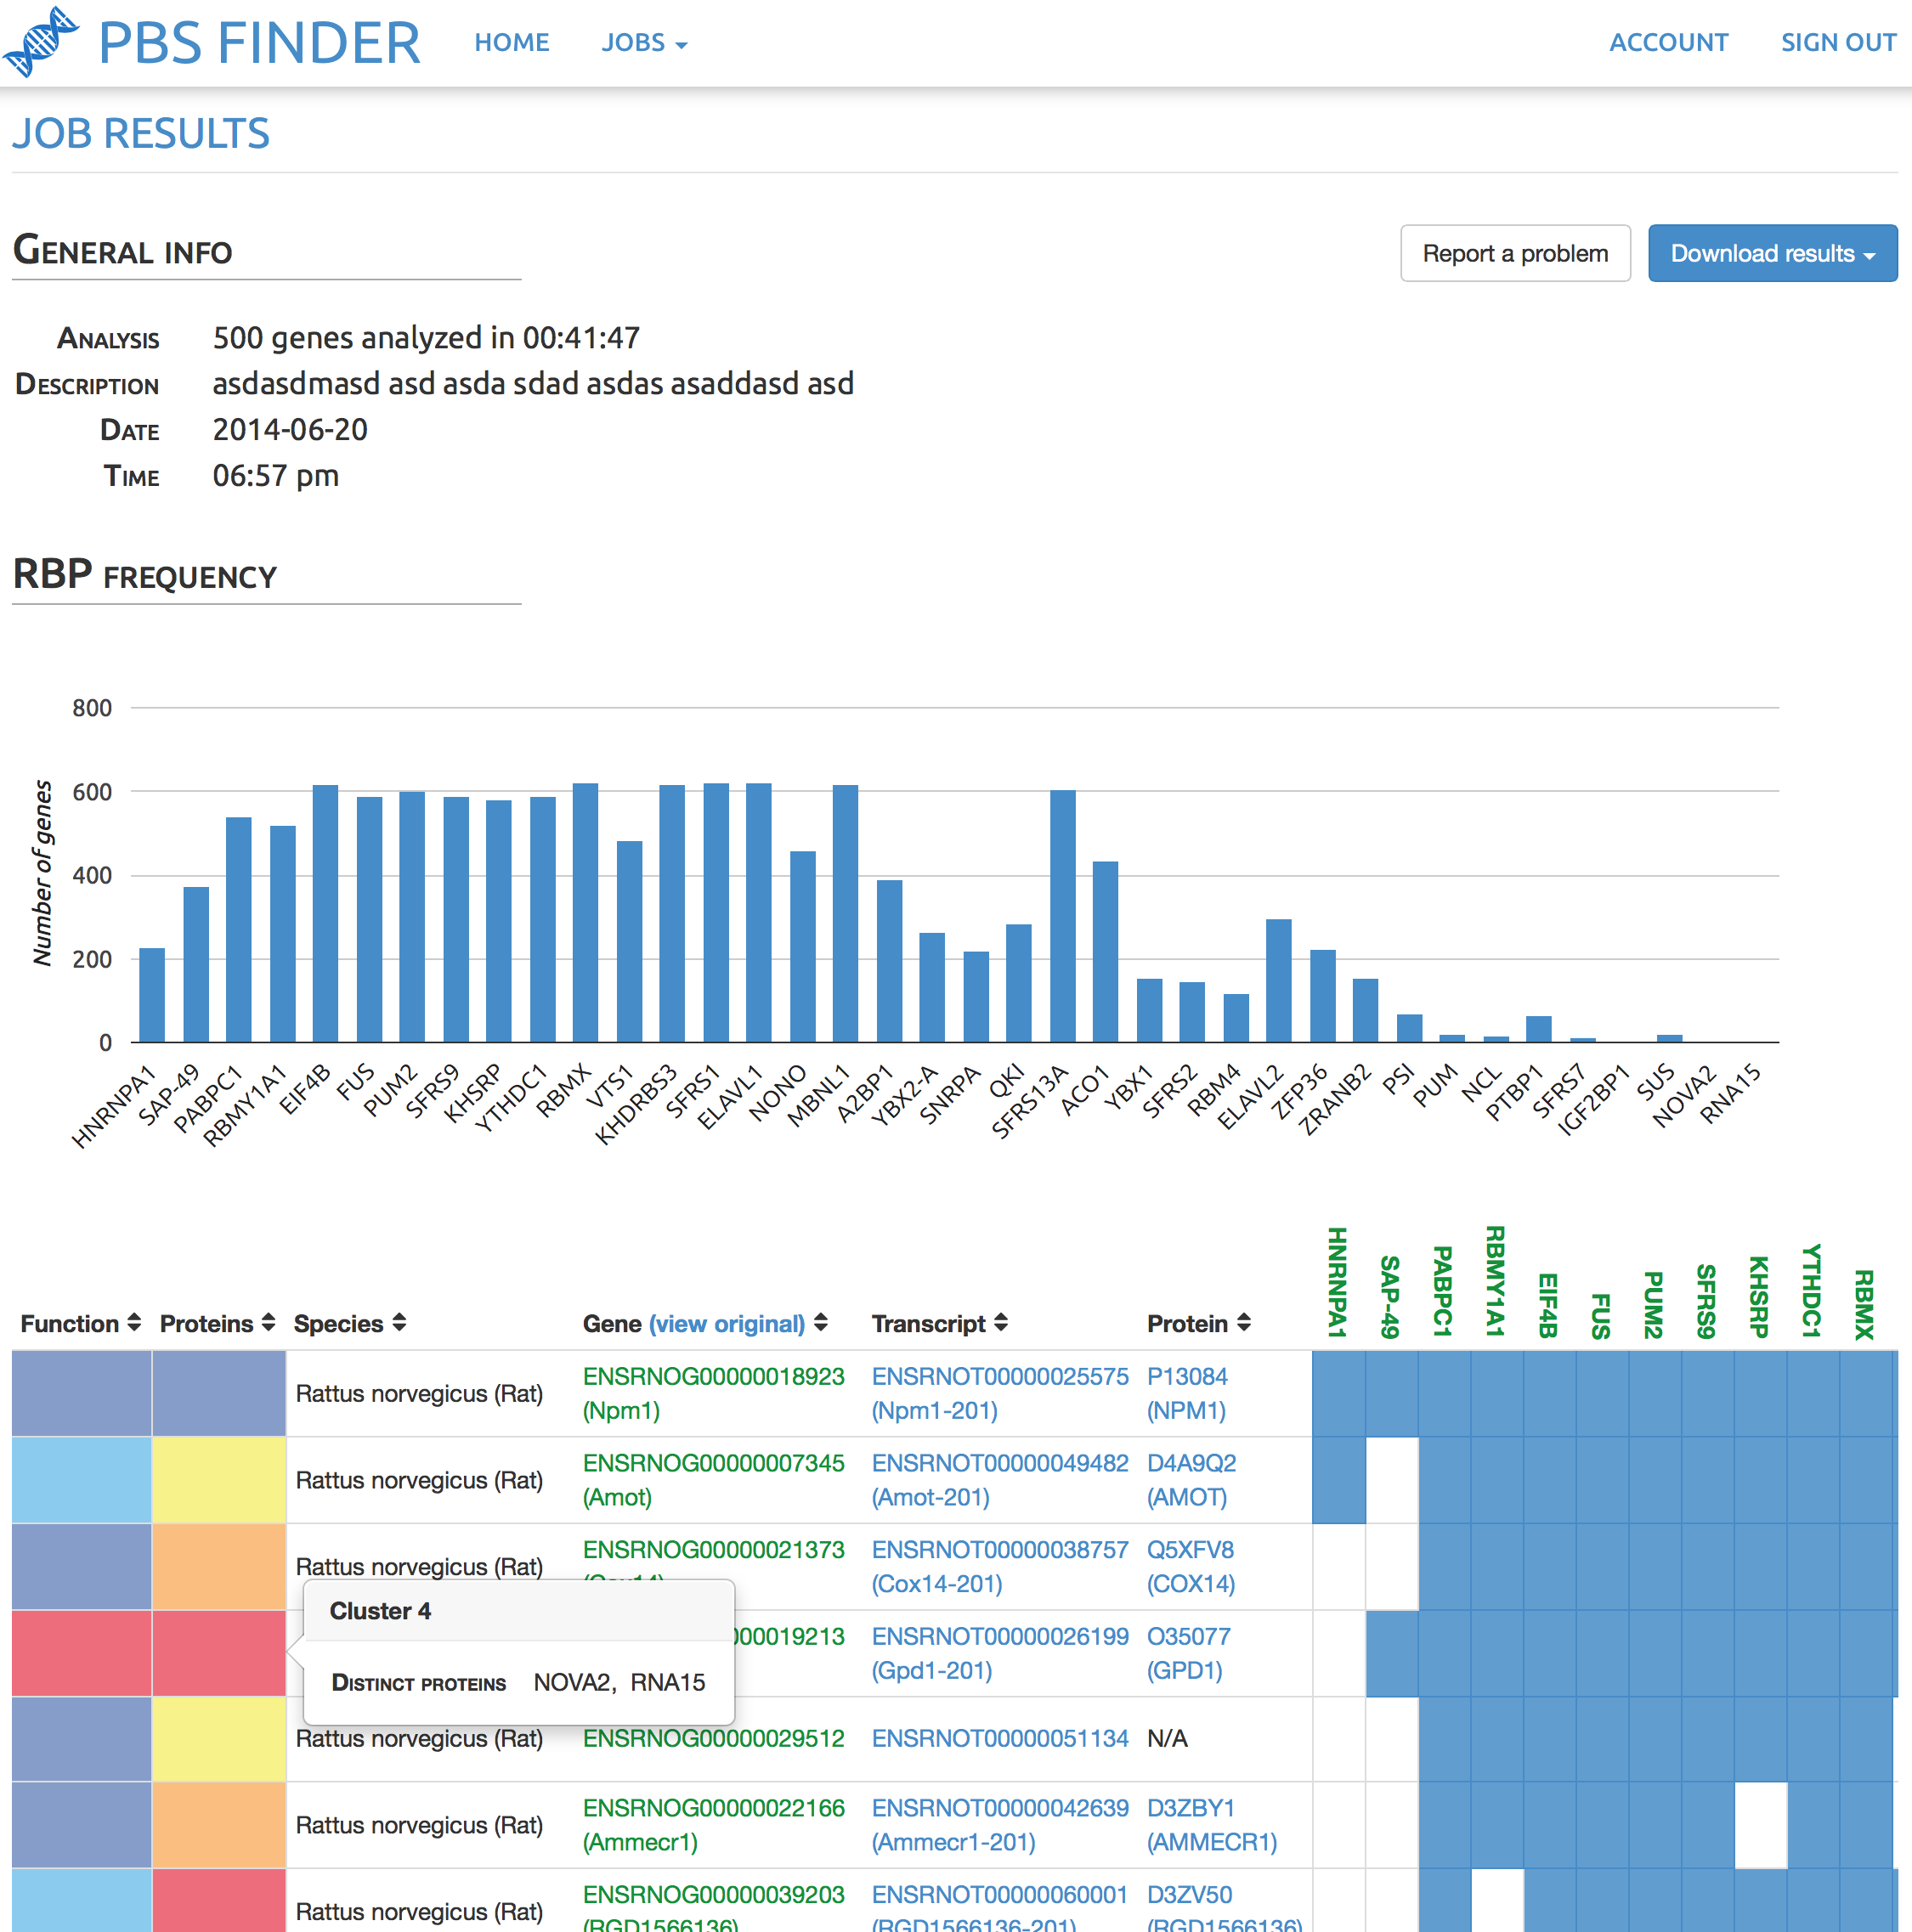
\includegraphics[width=\textwidth]{job_view}
    \caption[Job view example]{
      Job view example, also known as main view. It is comprised by three main
      components: general information (which includes data download); RBP
      frequency histogram; and RNA binding protein matching table.
    }
    \label{fig:job_view}
  \end{center}
\end{figure}

\subsubsection*{Transcript View}

The transcript view (Figure \ref{fig:trans_view}) offers more detailed
information about the transcript's binding proteins, giving for each protein the
base pairs that compose the binding site (and its start and stop positions) and
a percentage score of the match's quality. A maximum of three different genetic
sequences (5’ UTR, 3’ UTR and 3’ UTR downstream\footnote{5' UTR and 3' UTR are
non-coding regions located before the initiation codon and after the termination
codon, respectively. While these regions are not translated to useful genetic
products, their presence is important to regulate cellular processes.}) are also
displayed, depending on their availability. Whenever possible, related links to
other platforms are presented (Ensembl, NCBI and UniProt). Like the job view, it
also contains clustering information, but in this case only one column, that
shows how the RBPs related to that specific transcript were grouped. Also
similarly to the job view, users can click any group to obtain relevant
information about the defining characteristics of that particular group.

\begin{figure}[!htb]
  \begin{center}
    \leavevmode
    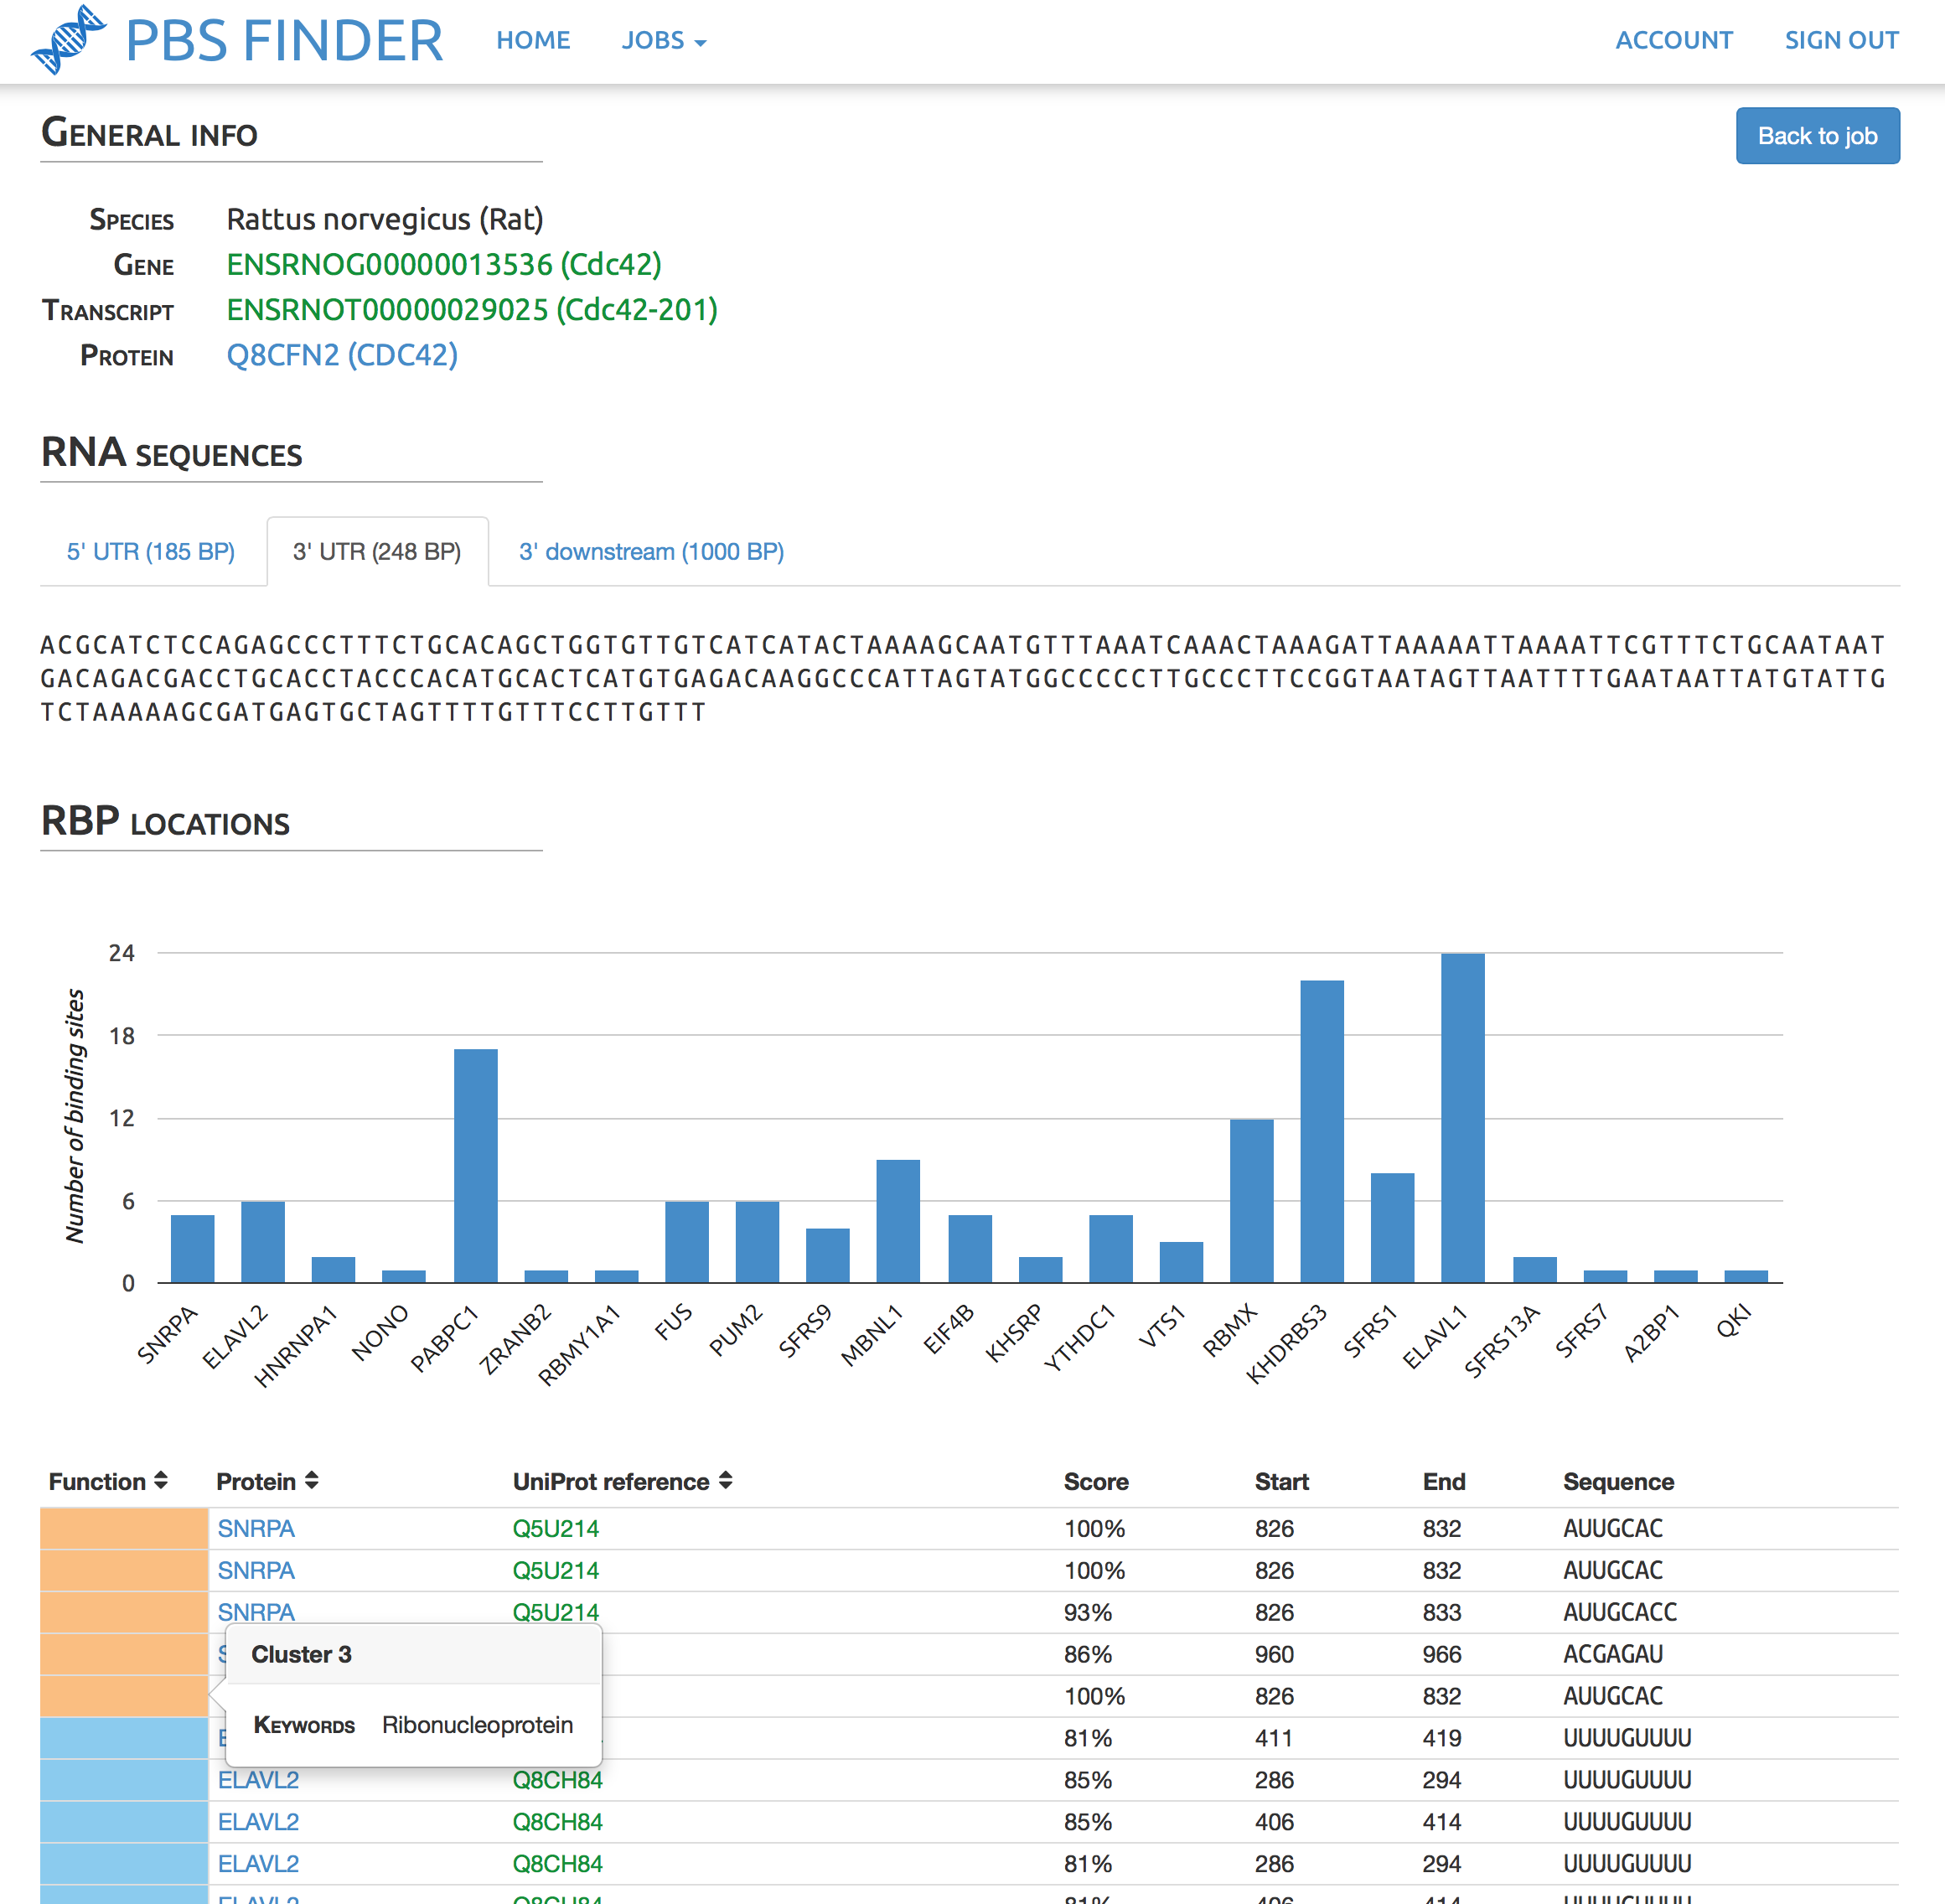
\includegraphics[width=\textwidth]{trans_view}
    \caption[Transcript view example]{
      Transcript view example. It contains four main areas: general information
      about the transcript; RNA sequences (5’UTR, 3’UTR and 3’UTR downstream are
      shown depending on availability); RBP locations histogram; and RBP
      location table (including clustering results and match sequences).
    }
    \label{fig:trans_view}
  \end{center}
\end{figure}

\subsubsection*{Protein View}

The protein view (Figure \ref{fig:prot_view}) displays relevant classification
information for every RBP (when available). This information includes the
protein's name, links to other platforms (UniProt, KEGG, Gene3D, etc.), tissues
in which the protein might be expressed, the protein's ontologies and the pathways
in which the protein participates. Each pathway is coupled with a link to the
corresponding KEGG pathway browser page.

\begin{figure}[!htb]
  \begin{center}
    \leavevmode
    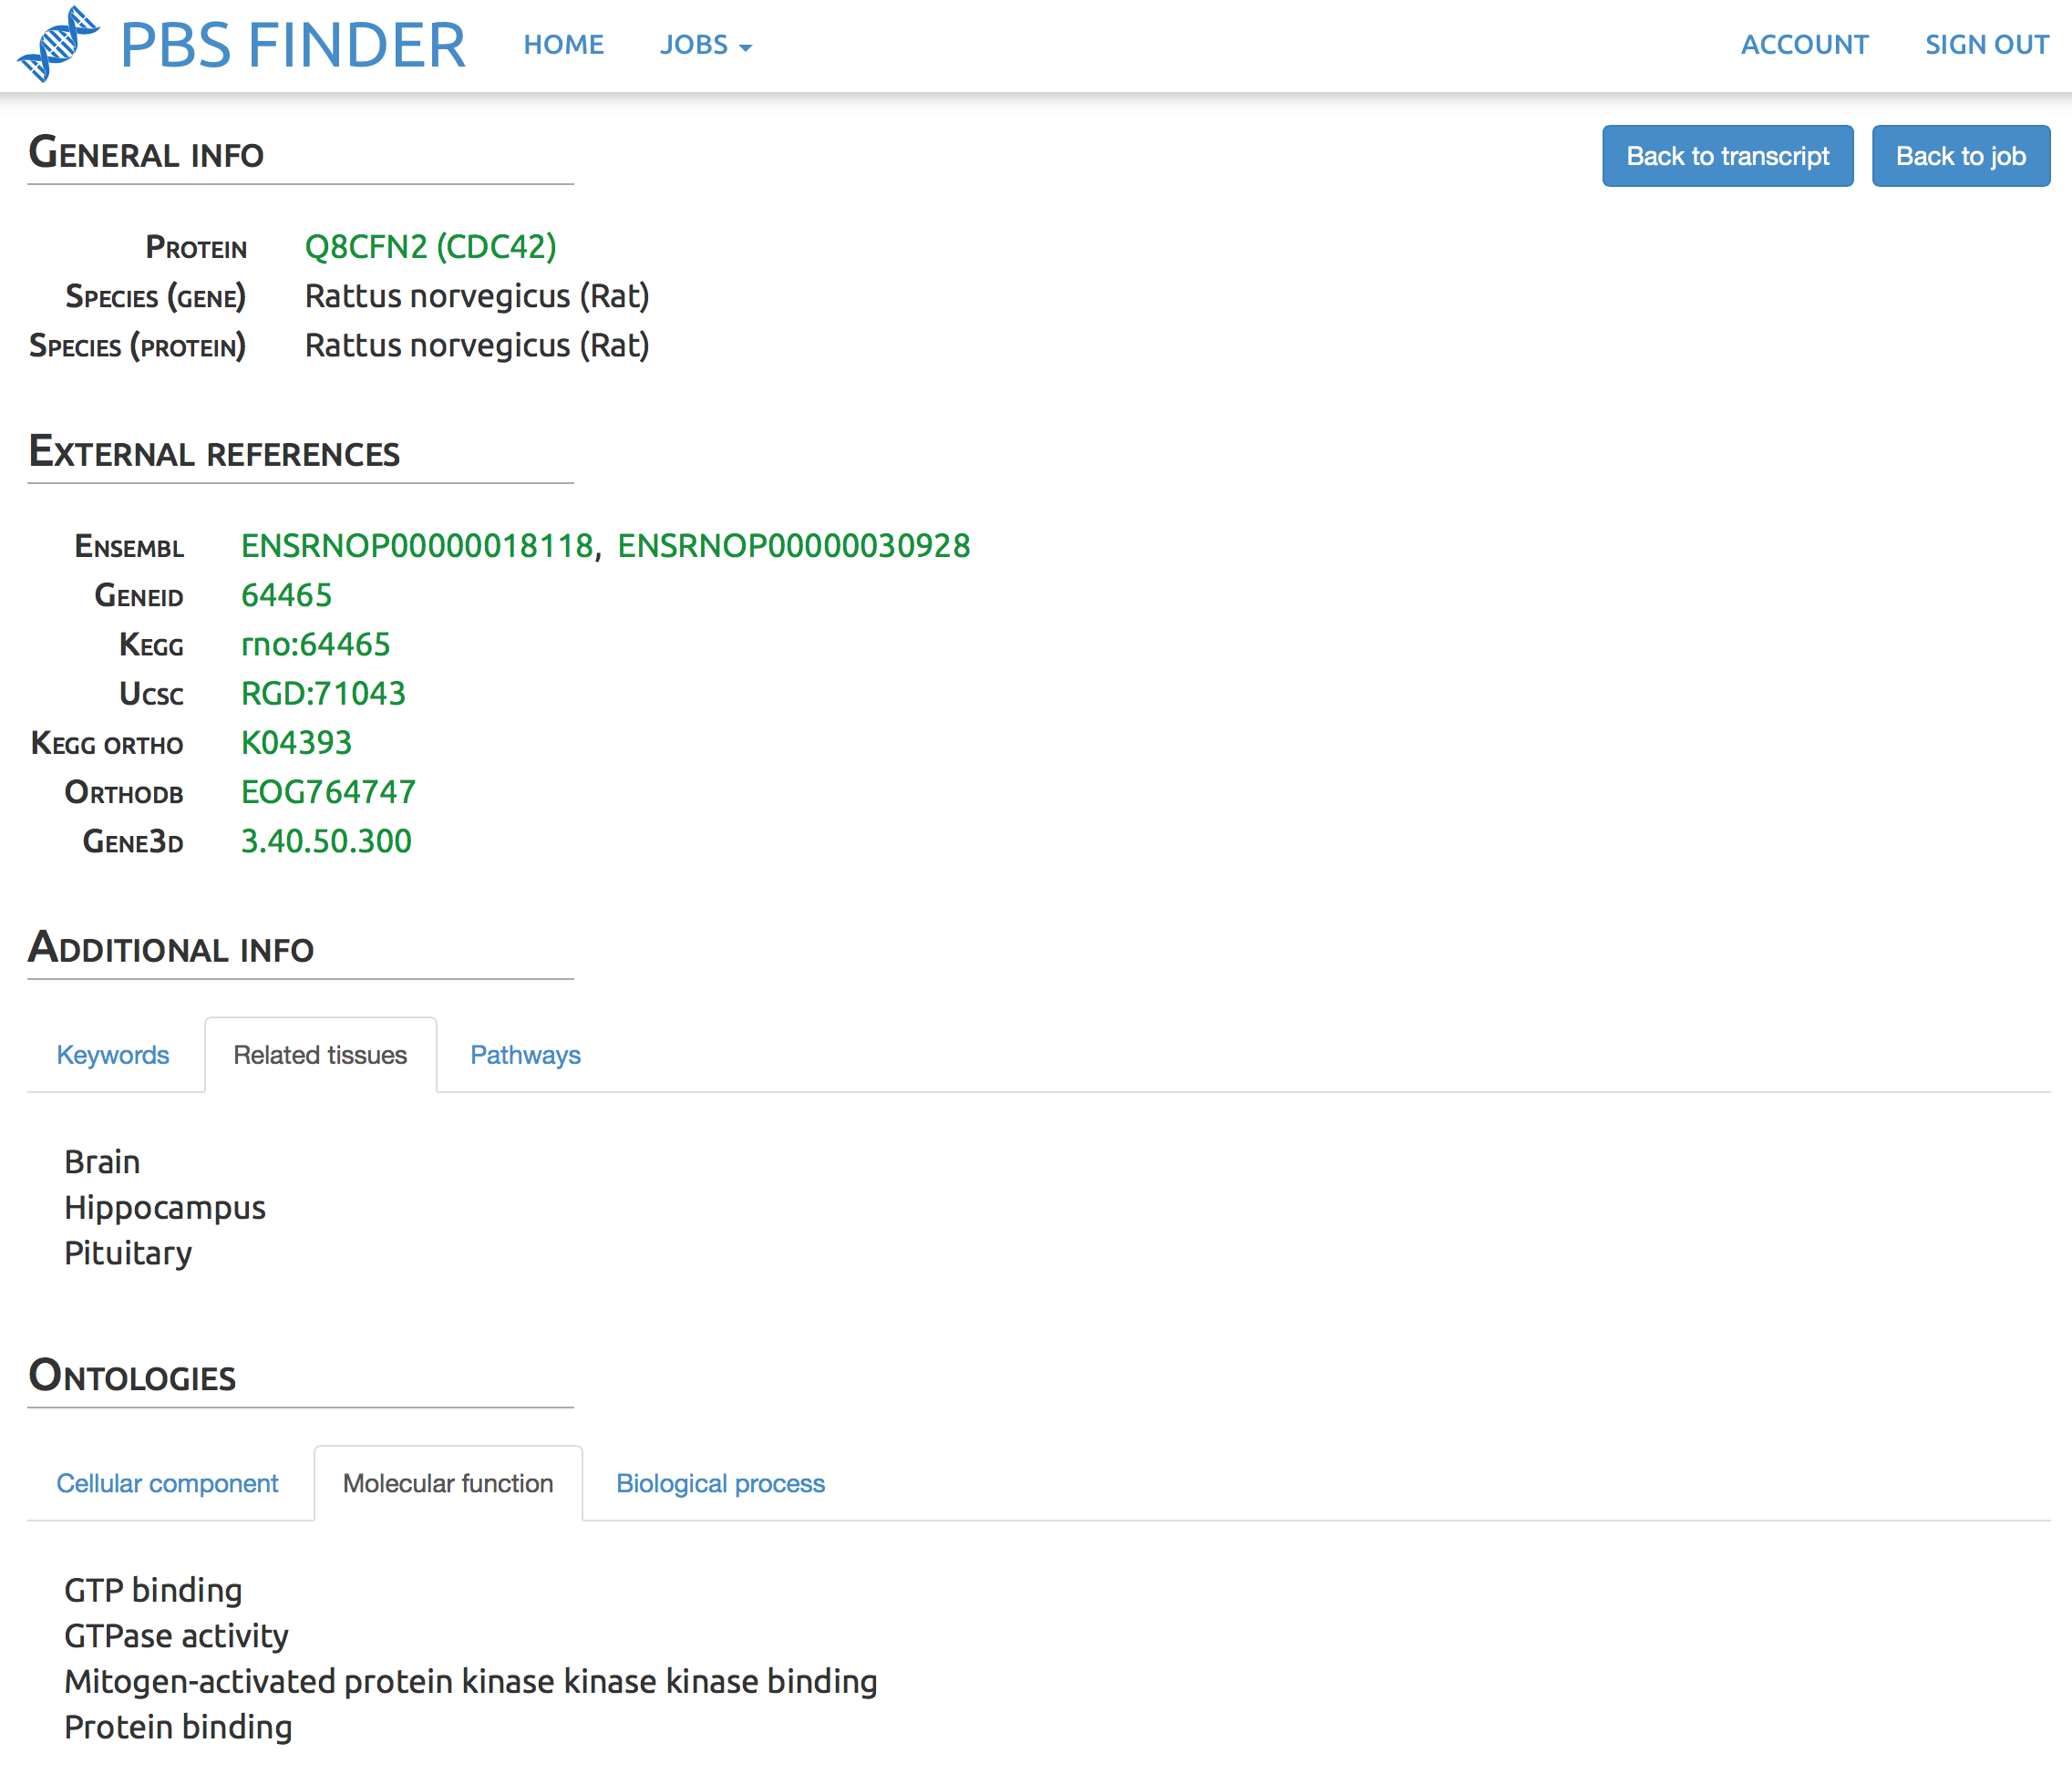
\includegraphics[width=\textwidth]{prot_view}
    \caption[Protein view example]{
      Protein view example, containing four relevant areas: general information
      about the protein; links to other web platforms with relevant information
      about the protein (note that some of those platforms might not contain
      information about a particular protein, and therefore no links can be
      shown); additional info, including keywords, related tissues and pathways
      in which the protein is expressed; and lastly, information about the
      protein's ontologies, including cellular components, molecular functions
      and biological processes.
    }
    \label{fig:prot_view}
  \end{center}
\end{figure}

\subsubsection*{Exporting the Results}

Besides browsing, users can download their results as text files. Three
different types of data projections of the results are provided: \emph{RBP
data}, \emph{protein data} and the \emph{complete data set}. RBP data can be
downloaded in either comma-separated values (CSV) or tab-separated values (TSV)
format. This file gives the user a match matrix of binding proteins, similar to
the one in the job results view, as well as species, gene and transcript
information. Protein data can also be downloaded in both CSV and TSV formats. It
gives a more complete view of the results, including species, gene, transcript
and protein identifiers and additional protein information (keywords, related
tissues, ontologies, etc.). Finally, the data set may be downloaded as a
complete Prolog predicate representation of the job results. This is the same
representation of the results that was created with the usage of ILP clustering
techniques in mind. While it was not possible to use those techniques, the
produced data set representation might still be of use to researchers.

While in most cases these data representation conversions are apparently
instantaneous, for large data sets they may take an additional amount of time.
This would cause the web application to seemingly block if the user tried to
download one of those files. To solve this problem all files are generated
during the analysis process, then stored in the web application's MongoDB
instance through GridFS\footnote{GridFS is a functionality integrated in MongoDB
that allows a simple file system to be simulated inside a database. Files are
divided into small chunks and those chunks are stored as regular MongoDB
documents.}. This allows those files to be downloaded instantly, as they need
only to be generated once.

%\section{Deployment}

%\begin{Notes}
%- Talk about tested deployment platforms.\\
%- Talk about system requirements.\\
%\end{Notes}

\section{Chapter Conclusions}

%\begin{Notes}
%- Generic chapter conclusion.\\
%\end{Notes}

In this chapter we presented a concrete approach to the development of the
proposed solutions. We reviewed their most important features and implementation
choices. Further examples of their usage is available through a case study in
Chapter \ref{chap:casestudy}.

\chapter{Case Study} \label{chap:casestudy}

\section*{}

In this chapter we present two case studies that were used as a proof of concept
for the developed system. We characterize the experimental environment, the used
data sets and the obtained results for both cases. We then compare the developed
solutions with the previously available methods.

\section{Gene Expression Analysis Pipeline}

\section{RNA Binding Protein Analysis Web Platform}

This case study is aimed at the RBP analysis tool (PBS Finder).
\emph{RhoGTPases} comprise a family of molecular switches that control signal
transduction pathways that link cell surface receptors to a variety of
intracellular responses. In this particular case the genes are related to the
species \emph{Rattus norvegicus}, commonly known as \emph{norway rat}.
\emph{Rattus norvegicus} is a model organism: a \qt{simple}, non-human organism
that is extensively studied, with the expectation that the discoveries made for
that particular organism are useful to understand different organisms
\cite{fields2005cell}. Other examples of model organisms are the \emph{E. coli}
bacteria, \emph{Drosophila melanogaster} (fruit fly) and \emph{Mus musculus}
(common mouse). This data set was produced by IBMC experts. The same experts
then validated the obtained results experimentally. The same experts then
validated the obtained results experimentally.

This experiment has three distinct goals. The first goal is to assess the
general usefulness of PBS Finder. It is important to determine if the developed
tool can at least reproduce the results obtained with previous methods. It is
also relevant to assess if PBS Finder is able to provide even more relevant
information to researchers, facilitating their work. The second goal is to
compare PBS Finder with the existing techniques of manual analysis. One of the
major constraints of manual analysis is the time it takes to complete; PBS
Finder should be able to reduce the duration of the analysis. Lastly, the third
goal is to assess the impact of differences in hardware performance in the
overall performance of the platform. PBS Finder should be sufficiently optimized
to be able to run in personal computers with decreased hardware performance,
instead of only in servers/computer clusters.

\subsection{Case Study Setup}

This case study is aimed only at the RBP analysis tool (PBS Finder). The reason
for this is that it was not possible to acquire a test data set in sufficient
time. It was also not possible to have an expert validate those results in the
available time. Moreover, the available case study data set was produced by IBMC
experts. The same experts then validated the obtained results experimentally.
The same experts then validated the obtained results experimentally.

\subsection{Analysis Data Set}

The analysis data set is comprised by twenty three gene identifiers, from the
\emph{RhoGTPase} family. The actual genes used for our tests can be found in
Table \ref{tab:genes}. Note that the tool only needs to receive gene
identifiers; gene names are not currently accepted as input data.

\begin{table}[!htb]
  \centering
  \begin{tabular}{{l}{l}{l}}
    \textbf{\emph{Gene name}} & \textbf{\emph{Gene ID}} & \textbf{\emph{Transcript ID}}\\ \hline
    Rhoj        & ENSRNOG00000021919 & ENSRNOT00000031979\\
    Rhog        & ENSRNOG00000020393 & ENSRNOT00000027641\\
    Rac3        & ENSRNOG00000048172 & ENSRNOT00000073886\\
    Rac2        & ENSRNOG00000007350 & ENSRNOT00000009994\\
    Rhod        & ENSRNOG00000019220 & ENSRNOT00000026092\\
    Rhof        & ENSRNOG00000042607 & ENSRNOT00000064390\\
    Rhoh        & ENSRNOG00000002540 & ENSRNOT00000003425\\
    Rnd         & ENSRNOG00000020698 & ENSRNOT00000028089\\
    Rhoc        & ENSRNOG00000012630 & ENSRNOT00000017254\\
    Cdc42       & ENSRNOG00000013536 & ENSRNOT00000029025\\
    Cdc42       & ENSRNOG00000013536 & ENSRNOT00000018118\\
    Rhoq        & ENSRNOG00000015415 & ENSRNOT00000020822\\
    Rac1        & ENSRNOG00000001068 & ENSRNOT00000001417\\
    Rhou        & ENSMUSG00000039960 & ENSMUST00000136615\\
    Rhou        & ENSMUSG00000039960 & ENSMUST00000045487\\
    Rhoa        & ENSRNOG00000050519 & ENSRNOT00000071664\\
    Rnd1        & ENSRNOG00000013621 & ENSRNOT00000018276\\
    Rnd3        & ENSRNOG00000004624 & ENSRNOT00000006111\\
    Rhob        & ENSRNOG00000021403 & ENSRNOT00000008008\\
    Rhobtb1     & ENSRNOG00000000633 & ENSRNOT00000000784\\
    Rhobtb2     & ENSRNOG00000017373 & ENSRNOT00000023876\\
    Rhobtb3     & ENSRNOG00000012414 & ENSRNOT00000016838\\
    Rhov        & ENSRNOG00000013380 & ENSRNOT00000018277\\ \hline
  \end{tabular}

  \caption[\emph{RhoGTPase} family genes used as data set in the case study]{
    \emph{RhoGTPase} family genes used as data set in the case study.
  }
  \label{tab:genes}
\end{table}

\subsection{Experimental Environment}

The testing environment was reproduced in two different machines. This machines
differ in their hardware and operative system, but every other variable in the
environment (internet connection speeds, machine usage, etc.) holds for both
machines. Performance results for the case study experiment for both machines
are given in Section \ref{sec:caseperf}. Henceforth the machines will be
referenced as \emph{machine1} and \emph{machine2}, as shown in Table
\ref{tab:specs}.

\begin{table}[!htb]
  \centering
  \begin{tabular}{{l} | {l}{l}}
    & \textbf{\emph{machine1}} & \textbf{\emph{machine2}}\\ \hline
    \textbf{\emph{Operative system}}    & OS X 10.9.3                     & Debian GNU/Linux Jessie/Sid\\
    \textbf{\emph{CPU}}                 & Intel Core i7 4850HQ (4 cores)  & Intel Core 2 Quad Q9400 (4 cores)\\
    \textbf{\emph{CPU speed}}           & 2.30 GHz                        & 2.66 GHz\\
    \textbf{\emph{Memory}}              & 16 GiB DDR3 (1600 MHz)          & 16 GiB DDR2 (800 MHz) \\
    \textbf{\emph{Internet connection}} & 100 Mbps                        & 100 Mbps\\ \hline
  \end{tabular}

  \caption[Specifications of the test environments used for the case study experiments]{
    Specifications of the test environments used for the case study experiments.
  }
  \label{tab:specs}
\end{table}

\subsection{Methodology}

In order for the experiments' execution time to depend only on the hardware of
the machines several environment restrictions were enforced. Firstly, it was
ensured that both machines were running their operative systems with the minimum
required applications, without any parallel usage. The network connections were
also checked to assert if they were working at equal speeds. Lastly, both
machines were verified in order to ascertain if all needed software had equal or
equivalent versions.

Ten experiments ran on each machine. These experiments were executed
sequentially rather than concurrently, to ensure more consistent results. Note
that access to the tool was barred to other users during these experiments for
the same reason. It was also ensured that the support structures of the
platform, including databases, were only used for this set of experiments and
reseted after each one.

\subsection{Results}

Table \ref{tab:results} includes the relevant results for this case study. As
expected, some RBPs are able to bind to almost all members of the
\emph{RhoGTPase} family (for example \emph{Muscleblind-Like Splicing Regulator
1} (MBNL1)), where others were more specific (for example \emph{Y Box Binding
Protein 1} (YBX1)). The latter kind is more interesting to analyse, as it might
be used to manipulate a very specific set of genes, while leaving all others
unaltered. In this case we chose the RBP YBX1 as the base of our validation,
both because it only interacts with five genes and because the genes it
interacts with are representative of the data set, in terms of biological
classification.

\begin{table}[!htb]
  \tiny
  \begin{tabular}{{l}{l} | {c}{c}{c}{c}{c}{c}{c}{c}{c}{c}{c}{c}}
    & & \textbf{\emph{SNRPA}} & \textbf{\emph{ELAVL2}} & \textbf{\emph{HNRNPA1}} & \textbf{\emph{NONO}} & \textbf{\emph{PABPC1}} & \textbf{\emph{ZRANB2}} & \textbf{\emph{RBMY1A1}} & \textbf{\emph{FUS}} & \textbf{\emph{PUM2}} & \textbf{\emph{SFRS9}} & \textbf{\emph{MBNL1}} & \textbf{\emph{EIF4B}}\\ \hline
    \parbox[t]{2mm}{\multirow{9}{*}{\rotatebox[origin=c]{90}{\emph{Cluster 1}}}}
    & \textbf{\emph{Rhoj}} &  &  &  & $\times$ & $\times$ &  & $\times$ & $\times$ & $\times$ & $\times$ & $\times$ & $\times$\\
    & \textbf{\emph{Rhog}} &  &  &  & $\times$ & $\times$ &  & $\times$ &  &  & $\times$ & $\times$ & $\times$\\
    & \textbf{\emph{Rac3}} &  &  & $\times$ & $\times$ & $\times$ &  & $\times$ & $\times$ & $\times$ & $\times$ & $\times$ & $\times$\\
    & \textbf{\emph{Rac2}} &  &  &  & $\times$ & $\times$ &  & $\times$ & $\times$ &  &  & $\times$ & $\times$\\
    & \textbf{\emph{Rhod}} &  &  & $\times$ &  & $\times$ &  &  & $\times$ & $\times$ & $\times$ & $\times$ & $\times$\\
    & \textbf{\emph{Rhof}} &  &  &  & $\times$ & $\times$ &  &  & $\times$ & $\times$ & $\times$ & $\times$ & $\times$\\
    & \textbf{\emph{Rhoh}} &  &  &  &  &  &  & $\times$ &  & $\times$ & $\times$ & $\times$ & $\times$\\
    & \textbf{\emph{Rnd2}} &  &  &  & $\times$ &  &  &  & $\times$ & $\times$ & $\times$ & $\times$ & $\times$\\
    & \textbf{\emph{Rhoc}} & $\times$ &  & $\times$ & $\times$ &  &  &  & $\times$ & $\times$ & $\times$ & $\times$ & $\times$\\ \\ \hline \\
    \parbox[t]{2mm}{\multirow{14}{*}{\rotatebox[origin=c]{90}{\emph{Cluster 2}}}}
    & \textbf{\emph{Cdc42}} & $\times$ & $\times$ & $\times$ & $\times$ & $\times$ & $\times$ & $\times$ & $\times$ & $\times$ & $\times$ & $\times$ & $\times$\\
    & \textbf{\emph{Cdc42}} &  & $\times$ &  & $\times$ &  &  & $\times$ & $\times$ & $\times$ & $\times$ & $\times$ & $\times$\\
    & \textbf{\emph{Rhoq}} & $\times$ &  &  & $\times$ & $\times$ &  & $\times$ & $\times$ & $\times$ & $\times$ & $\times$ & $\times$\\
    & \textbf{\emph{Rac1}} & $\times$ &  &  &  & $\times$ &  &  & $\times$ & $\times$ & $\times$ & $\times$ & $\times$\\
    & \textbf{\emph{Rhou}} &  &  &  &  &  &  &  &  &  &  &  & \\
    & \textbf{\emph{Rhou}} & $\times$ & $\times$ & $\times$ & $\times$ & $\times$ &  & $\times$ & $\times$ & $\times$ & $\times$ & $\times$ & $\times$\\
    & \textbf{\emph{Rhoa}} &  & $\times$ &  &  & $\times$ &  &  & $\times$ & $\times$ & $\times$ & $\times$ & $\times$\\
    & \textbf{\emph{Rnd1}} &  &  &  & $\times$ & $\times$ &  &  & $\times$ &  & $\times$ & $\times$ & $\times$\\
    & \textbf{\emph{Rnd3}} &  & $\times$ &  & $\times$ & $\times$ &  & $\times$ & $\times$ & $\times$ & $\times$ & $\times$ & $\times$\\
    & \textbf{\emph{Rhob}} & $\times$ & $\times$ &  & $\times$ & $\times$ &  & $\times$ & $\times$ & $\times$ & $\times$ & $\times$ & $\times$\\
    & \textbf{\emph{Rhobtb1}} & $\times$ & $\times$ & $\times$ & $\times$ & $\times$ & $\times$ & $\times$ & $\times$ & $\times$ & $\times$ & $\times$ & $\times$\\
    & \textbf{\emph{Rhobtb2}} &  &  &  & $\times$ &  &  &  & $\times$ & $\times$ & $\times$ & $\times$ & $\times$\\
    & \textbf{\emph{Rhobtb3}} & $\times$ & $\times$ & $\times$ & $\times$ & $\times$ & $\times$ & $\times$ & $\times$ & $\times$ & $\times$ & $\times$ & $\times$\\
    & \textbf{\emph{Rhov}} &  &  &  & $\times$ & $\times$ &  & $\times$ & $\times$ & $\times$ & $\times$ & $\times$ & $\times$\\ \hline
  \end{tabular}

  \vspace{0.4cm}

  \begin{tabular}{{l}{l} | {c}{c}{c}{c}{c}{c}{c}{c}{c}{c}{c}{c}}
    & & \textbf{\emph{EIF4B}} & \textbf{\emph{KHSRP}} & \textbf{\emph{YTHDC1}} & \textbf{\emph{VTS1}} & \textbf{\emph{RBMX}} & \textbf{\emph{KHDRBS3}} & \textbf{\emph{SFRS1}} & \textbf{\emph{ELAVL1}} & \textbf{\emph{SFRS13A}} & \textbf{\emph{SFRS7}} & \textbf{\emph{A2BP1}} & \textbf{\emph{QKI}}\\ \hline
    \parbox[t]{2mm}{\multirow{9}{*}{\rotatebox[origin=c]{90}{\emph{Cluster 1}}}}
    & \textbf{\emph{Rhoj}} & $\times$ & $\times$ & $\times$ & $\times$ & $\times$ & $\times$ & $\times$ & $\times$ & $\times$ &  & $\times$ & $\times$\\
    & \textbf{\emph{Rhog}} & $\times$ & $\times$ & $\times$ &  & $\times$ & $\times$ & $\times$ & $\times$ & $\times$ &  &  & $\times$\\
    & \textbf{\emph{Rac3}} & $\times$ & $\times$ & $\times$ & $\times$ & $\times$ & $\times$ & $\times$ & $\times$ & $\times$ &  & $\times$ & $\times$\\
    & \textbf{\emph{Rac2}} & $\times$ & $\times$ & $\times$ &  & $\times$ & $\times$ & $\times$ & $\times$ & $\times$ &  &  & \\
    & \textbf{\emph{Rhod}} & $\times$ & $\times$ & $\times$ & $\times$ & $\times$ & $\times$ & $\times$ & $\times$ & $\times$ &  & $\times$ & $\times$\\
    & \textbf{\emph{Rhof}} & $\times$ & $\times$ & $\times$ & $\times$ & $\times$ & $\times$ & $\times$ & $\times$ & $\times$ &  &  & $\times$\\
    & \textbf{\emph{Rhoh}} & $\times$ & $\times$ &  &  & $\times$ & $\times$ & $\times$ & $\times$ & $\times$ &  &  & \\
    & \textbf{\emph{Rnd2}} & $\times$ & $\times$ & $\times$ & $\times$ & $\times$ & $\times$ & $\times$ & $\times$ & $\times$ &  & $\times$ & \\
    & \textbf{\emph{Rhoc}} & $\times$ & $\times$ & $\times$ & $\times$ & $\times$ & $\times$ & $\times$ & $\times$ & $\times$ &  & $\times$ & \\ \\ \hline \\
    \parbox[t]{2mm}{\multirow{14}{*}{\rotatebox[origin=c]{90}{\emph{Cluster 2}}}}
    & \textbf{\emph{Cdc42}} & $\times$ & $\times$ & $\times$ & $\times$ & $\times$ & $\times$ & $\times$ & $\times$ & $\times$ & $\times$ & $\times$ & $\times$\\
    & \textbf{\emph{Cdc42}} & $\times$ & $\times$ & $\times$ &  & $\times$ & $\times$ & $\times$ & $\times$ & $\times$ &  & $\times$ & $\times$\\
    & \textbf{\emph{Rhoq}} & $\times$ & $\times$ & $\times$ & $\times$ & $\times$ & $\times$ & $\times$ & $\times$ & $\times$ &  & $\times$ & $\times$\\
    & \textbf{\emph{Rac1}} & $\times$ & $\times$ & $\times$ & $\times$ & $\times$ & $\times$ & $\times$ & $\times$ & $\times$ &  &  & $\times$\\
    & \textbf{\emph{Rhou}} &  &  &  &  &  &  &  &  &  &  &  & \\
    & \textbf{\emph{Rhou}} & $\times$ & $\times$ & $\times$ & $\times$ & $\times$ & $\times$ & $\times$ & $\times$ & $\times$ &  & $\times$ & \\
    & \textbf{\emph{Rhoa}} & $\times$ & $\times$ & $\times$ & $\times$ & $\times$ & $\times$ & $\times$ & $\times$ & $\times$ &  &  & $\times$\\
    & \textbf{\emph{Rnd1}} & $\times$ & $\times$ &  & $\times$ & $\times$ & $\times$ & $\times$ & $\times$ & $\times$ &  & $\times$ & \\
    & \textbf{\emph{Rnd3}} & $\times$ & $\times$ & $\times$ & $\times$ & $\times$ & $\times$ & $\times$ & $\times$ & $\times$ &  & $\times$ & \\
    & \textbf{\emph{Rhob}} & $\times$ & $\times$ & $\times$ & $\times$ & $\times$ & $\times$ & $\times$ & $\times$ & $\times$ & $\times$ & $\times$ & \\
    & \textbf{\emph{Rhobtb1}} & $\times$ & $\times$ & $\times$ & $\times$ & $\times$ & $\times$ & $\times$ & $\times$ & $\times$ &  & $\times$ & \\
    & \textbf{\emph{Rhobtb2}} & $\times$ & $\times$ &  & $\times$ & $\times$ &  & $\times$ & $\times$ & $\times$ &  &  & \\
    & \textbf{\emph{Rhobtb3}} & $\times$ & $\times$ & $\times$ & $\times$ & $\times$ & $\times$ & $\times$ & $\times$ & $\times$ &  & $\times$ & $\times$\\
    & \textbf{\emph{Rhov}} & $\times$ & $\times$ & $\times$ & $\times$ & $\times$ & $\times$ & $\times$ & $\times$ & $\times$ &  &  & \\ \hline
  \end{tabular}

  \vspace{0.4cm}

  \begin{tabular}{{l}{l} | {c}{c}{c}{c}{c}{c}{c}{c}{c}{c}{c}{c}}
    & & \textbf{\emph{QKI}} & \textbf{\emph{SUS}} & \textbf{\emph{YBX2-A}} & \textbf{\emph{PSI}} & \textbf{\emph{SAP-49}} & \textbf{\emph{ACO1}} & \textbf{\emph{YBX1}} & \textbf{\emph{SFRS2}} & \textbf{\emph{ZFP36}} & \textbf{\emph{RBM4}} & \textbf{\emph{PTBP1}}\\ \hline
    \parbox[t]{2mm}{\multirow{9}{*}{\rotatebox[origin=c]{90}{\emph{Cluster 1}}}}
    & \textbf{\emph{Rhoj}} & $\times$ &  & $\times$ &  & $\times$ &  & $\times$ & $\times$ &  &  & \\
    & \textbf{\emph{Rhog}} & $\times$ &  &  &  &  & $\times$ &  &  &  &  & \\
    & \textbf{\emph{Rac3}} & $\times$ &  &  &  &  &  &  &  &  &  & \\
    & \textbf{\emph{Rac2}} &  &  & $\times$ &  &  &  &  &  &  &  & \\
    & \textbf{\emph{Rhod}} & $\times$ &  &  &  &  &  &  &  &  &  & \\
    & \textbf{\emph{Rhof}} & $\times$ &  &  &  &  & $\times$ &  & $\times$ &  & $\times$ & \\
    & \textbf{\emph{Rhoh}} &  &  &  &  &  &  &  &  &  &  & \\
    & \textbf{\emph{Rnd2}} &  &  &  &  &  & $\times$ &  & $\times$ &  &  & \\
    & \textbf{\emph{Rhoc}} &  &  &  &  &  &  &  &  &  &  & \\ \\ \hline \\
    \parbox[t]{2mm}{\multirow{14}{*}{\rotatebox[origin=c]{90}{\emph{Cluster 2}}}}
    & \textbf{\emph{Cdc42}} & $\times$ &  &  &  &  &  &  &  &  &  & \\
    & \textbf{\emph{Cdc42}} & $\times$ & $\times$ & $\times$ & $\times$ & $\times$ & $\times$ & $\times$ &  &  &  & \\
    & \textbf{\emph{Rhoq}} & $\times$ &  & $\times$ &  & $\times$ & $\times$ &  &  & $\times$ & $\times$ & \\
    & \textbf{\emph{Rac1}} & $\times$ &  & $\times$ &  & $\times$ & $\times$ &  &  &  & $\times$ & \\
    & \textbf{\emph{Rhou}} &  &  &  &  &  &  &  &  &  &  & \\
    & \textbf{\emph{Rhou}} &  &  & $\times$ &  & $\times$ & $\times$ &  &  & $\times$ &  & \\
    & \textbf{\emph{Rhoa}} & $\times$ &  &  &  & $\times$ & $\times$ & $\times$ &  &  & $\times$ & \\
    & \textbf{\emph{Rnd1}} &  &  &  &  &  & $\times$ &  &  & $\times$ &  & \\
    & \textbf{\emph{Rnd3}} &  &  &  & $\times$ & $\times$ & $\times$ & $\times$ &  &  &  & $\times$\\
    & \textbf{\emph{Rhob}} &  &  &  &  & $\times$ & $\times$ &  &  &  & $\times$ & \\
    & \textbf{\emph{Rhobtb1}} &  &  &  &  &  & $\times$ & $\times$ &  &  & $\times$ & \\
    & \textbf{\emph{Rhobtb2}} &  &  & $\times$ &  &  & $\times$ &  &  &  &  & \\
    & \textbf{\emph{Rhobtb3}} & $\times$ &  & $\times$ &  & $\times$ & $\times$ &  & $\times$ & $\times$ &  & \\
    & \textbf{\emph{Rhov}} &  &  &  &  & $\times$ & $\times$ &  &  &  &  & \\ \hline
  \end{tabular}

  \caption[Case study results generated by PBS Finder]{
    Case study results generated by PBS Finder (table divided intro three
    sections for legibility). Each row represents a single gene from the data
    set and each row represents an RBP with which the genes potentially bind.
    Note that for this particular analysis the tool divided the genes into two
    clusters, joining together genes that bind with similar proteins.
  }
  \label{tab:results}
\end{table}

Table \ref{tab:results} shows that the tool found two clusters of genes within
the data set. In this case the best results were obtained using average linkage
hierarchical clustering, coupled with a binary representation of the distance
matrix. This particular solution was chosen for having a higher average
silhouette than other produced solutions. Table \ref{tab:differ} contains a list
of all the proteins that were considered as defining for their clusters. Note
that \emph{Cluster 1} contained almost exclusively proteins that were frequent
across the data set; on the other hand, \emph{Cluster 2} contained seven RBPs
that were identified as features of that cluster.

\begin{table}[!htb]
  \centering
  \begin{tabular}{{c} | {l}}
    \textbf{\emph{Cluster 1}} & \textbf{\emph{Cluster 2}}\\ \hline
    \multirow{7}{*}{-}
    & ZFP36 \\
    & ELAVL2 \\
    & ZRANB2 \\
    & PSI \\
    & PTBP1 \\
    & SFRS7 \\
    & SUS \\ \hline
  \end{tabular}

  \caption[RBPs found to characterize each cluster]{
    RBPs found to characterize each cluster. Note that \emph{Cluster 1} does not
    contain any RBP that can be considered as a defining feature of that
    cluster. This is due to the fact that proteins in \emph{Cluster 1} are
    generally abundant through the data set.
  }
  \label{tab:perf}
\end{table}




\subsection{Correctness and Completeness of the Results}\label{sec:caseval}

Result checking was conducted in two different fronts: \emph{collected data
completeness and correction}; and \emph{biological results evaluation}.

Completeness and correction analysis were conducted both manually and
automatically during the development of the tool. In some cases it was possible
to automate these validations using \emph{unit testing}\footnote{Unit testing is
a software testing method that focus on testing individual units of a developed
software; these tests are used to assess which of those units are fit, and which
do not work correctly.} and \emph{mocks}\footnote{A mock, or mock object, is a
simulated object that mimics the behavior of a complex component of a software
system. Mock objects are particularly useful when the behavior of its real
counterpart is hard/costly to predict and control}. However, creating this test
infrastructure is a lengthy process. As such, some results, as is the case with
this case study, were manually validated. This validation involves manually
visiting every website used to collect information and cross reference that
information with the one collected by the tool.

The validation of biological results is more complex. It involves experimentally
obtaining the same information that the tool produces, from biological samples.
This validation was conducted at IBMC. However, it is a lengthy process, as
obtaining this information may take several weeks. It has two main objectives:
validating the number and type of RBPs that bind to each gene; and validate the
adequacy of the gene clustering results.

Both checking processes were conducted successfully, thus improving the
confidence that the developed platform produces adequate results.

\subsection{Comparison with Previous Method}\label{sec:caseperf}

As with any newly developed automation tool, it is essential to assess if the
developed tool is in fact an improvement over previously available methods. The
results produced by the tool were already determined correct in Section
\ref{sec:caseval}. As such, the tool should now be evaluated from the user
experience standpoint, namely, in terms of \emph{task simplification} and
\emph{efficiency}.

\subsubsection*{Task Simplification}

Figure \ref{fig:oldvsnew} depicts how PBS Finder simplified the analysis process,
from the user point of view. When conducting a manual analysis, the user must
individually analyse every gene in the data set.

\begin{figure}[!htb]
  \begin{center}
    \leavevmode
    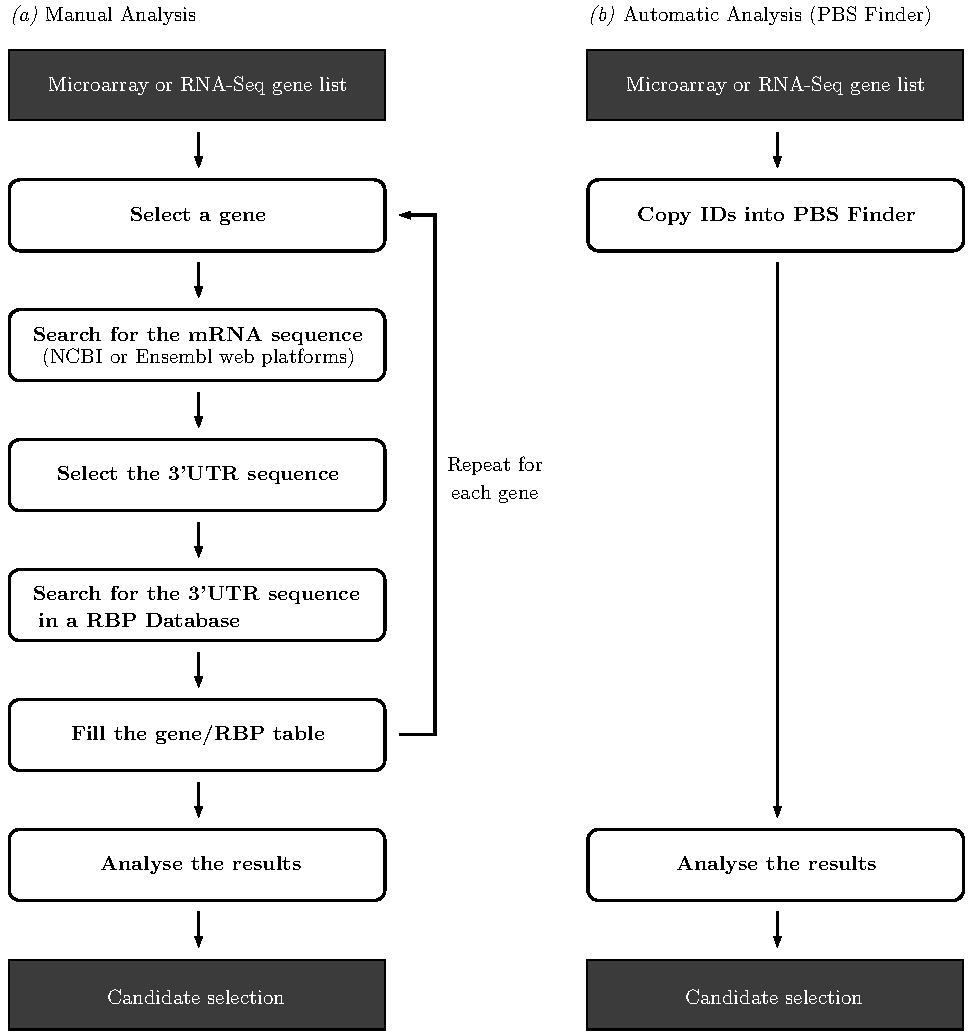
\includegraphics[width=\textwidth]{oldvsnew}
    \caption[Comparison between manual RBP analysis and automatic RBP analysis (conducted with PBS Finder)]{
      Comparison between manual RBP analysis and automatic RBP analysis
      (conducted with PBS Finder).
    }
    \label{fig:oldvsnew}
  \end{center}
\end{figure}

The first step is to select a gene for analysis. The gene identifier is then
searched in either Ensembl or NCBI web platforms, depending on the type of the
identifier. If the gene is found in those platforms, the next step involves
finding the 3'UTR sequence in the results page and copying it. That sequence is
then passed to an online RBP analysis platform, that should retrieve a list of
RBPs that may bind to that particular sequence. Lastly, the RBP information must
be manually combined in the results table. When this information is collected
for every gene it is finally possible to conduct a useful analysis.

On the other hand, with PBS Finder the user needs only to provide the complete
list of all gene identifiers in the data set. The tool will them automatically
process those identifiers, find all relevant information and present it to the
user, ready for further analysis. Note that these results contain additional
information that is not available in the manual analysis: gene, transcript and
protein information (names, additional sequences, pathways, etc.); links to
external platforms; useful histograms; and gene and protein clustering results.

\subsubsection*{Efficiency}

It is essential for the developed platform to be able to conduct the analysis in
a timely fashion, making tool performance a major concern. As such, we compared
the average time that an expert would take to analyse the data set to the
average time that the tool takes to analyse the same data set.

The consulted molecular biology expert estimated that, on average, it would take
thirty minutes to analyse a single gene. This means that an expert would need an
average of eleven and a half hours ($30\ minutes \times 23\ genes$) to process the
entire case study data set.

On the other hand, the automated tool takes a shorter amount of time to conduct
the analysis of the same data set. In order to assess the actual amount of time
the tool took to analyse the entire data set we ran twenty sequential
experiences, ten for each of the experimental environments. Table \ref{tab:perf}
depicts the duration of each one of those experiments, as well as their average
duration. As expected, an automated tool widely outperforms a human expert in
information collection and analysis.

\begin{table}[!htb]
  \centering
  \begin{tabular}{{l} | {l}{l}}
    & \textbf{\emph{machine1}} & \textbf{\emph{machine2}}\\ \hline
    \textbf{\emph{Experience 1}}    & $1m\ 47s$ & $6m\ 34s$\\
    \textbf{\emph{Experience 2}}    & $1m\ 58s$ & $6m\ 25s$\\
    \textbf{\emph{Experience 3}}    & $1m\ 46s$ & $6m\ 30s$\\
    \textbf{\emph{Experience 4}}    & $1m\ 45s$ & $6m\ 15s$\\
    \textbf{\emph{Experience 5}}    & $2m\ 23s$ & $6m\ 42s$\\
    \textbf{\emph{Experience 6}}    & $1m\ 35s$ & $6m\ 30s$\\
    \textbf{\emph{Experience 7}}    & $1m\ 40s$ & $6m\ 31s$\\
    \textbf{\emph{Experience 8}}    & $1m\ 39s$ & $6m\ 11s$\\
    \textbf{\emph{Experience 9}}    & $1m\ 42s$ & $6m\ 42s$\\
    \textbf{\emph{Experience 10}}   & $1m\ 42s$ & $6m\ 52s$\\ \hline
    \textbf{\emph{Average time}}    & $1m\ 42s$ & $6m\ 31s$\\ \hline
  \end{tabular}

  \caption[Execution times of the case study data set in two different environments]{
    Execution times of the case study data set in two different environments
    (sequential experiments). Note that while \emph{machine2} has a significant
    loss in performance (due to its outdated hardware) it still achieves
    satisfactory execution times. This test also shows that it is possible to
    efficiently run PBS Finder in a home computer.
  }
  \label{tab:perf}
\end{table}

Table \ref{tab:stress} contains the stress test results of both machines,
compared to the estimated work time needed by an expert. In this case stress
tests were executed with one hundred, five hundred and nine hundred gene
identifiers. Even the slowest test can be completed by the machine with less
performance (\emph{machine2}) in under three hours. That same effort would take
an expert approximately four hundred and fifty hours, which amounts to two and a
half weeks on a twenty four hour working day, and to just under two months in
normal working conditions (eight hours per day).

\begin{table}[!htb]
  \centering
  \begin{tabular}{{l} | {l}{l}{l}}
    \textbf{\emph{Number of IDs}} & \textbf{\emph{machine1}} & \textbf{\emph{machine2}} & \textbf{\emph{Manual method}} \\ \hline
    100  & $9m\ 56s$          & $11m\ 1s$      & $\approx 50h$\\
    500   & $41m\ 47s$         & $55m\ 51s$     & $\approx 250h$\\
    900   & $1h\ 33m\ 32s$     & $2h\ 7m\ 4s$   & $\approx 450h$\\ \hline
  \end{tabular}

  \caption[Results comparison between manual analysis and both test machines]{
    Results comparison between manual analysis and both test machines.
  }
  \label{tab:stress}
\end{table}

\subsection{Chapter Conclusions}

Through this case study we have shown that PBS Finder produces relevant and
correct results for large-scale analysis of RBPs using data from \ngs{}
techniques. We have also shown that our tool significantly facilitates the work
of the biologist, by making analysis of this data easier and quicker. As such,
we consider PBS Finder a tool of great value for studying RNA biology.


\chapter{Conclusions} \label{chap:conclusions}

\section*{}

%\begin{Notes}
%- Check PDIS conclusion.\\
%- Talk about finishing iRAP's web integration and further exploration of its
%results.\\
%- Talk about full automated integration between both tools.\\
%\end{Notes}

In this thesis we proposed the development of an integrated platform for RNA-Seq
data analysis. This platform is able to perform the entirety of the analysis
process, from the sequencing reads, to grouping genes by their RBPs. This means
being able to perform read alignment, quantification and differential expression
analysis tasks, as well as data set enrichment, RBP identification and
clustering analysis of genes and proteins. Through a case study we showed the
developed prototype in action, and assessed its correctness and efficiency.
Below we will share our thoughts on the fulfilment of the objectives of this
thesis, and present some possibilities for any future development in our
solution.

\section{Objective Fulfilment}

Our objectives, in terms of studying the problem at hand and developing a
solution to it, were completely fulfilled. The proposed solution corresponds to
all of our expectations. However, as previously discussed, the implementation of
the RNA-Seq data analysis pipeline system was not completed, due to time
constraints. As such, our objective of prototyping and testing the complete
system could not be completely achieved.

\section{Future Work}

The obvious continuation of the proposed work would be to finish the
implementation and integration of the RNA-Seq data analysis pipeline. This would
allow our solution to work as designed, integrating the complete analysis
pipeline, from sequencing data to gene clustering and result visualization.
Furthermore, it would be interesting to study the developed tools in terms of
performance, under large volumes of information and requests. Whilst the tools
were developed taking in consideration their performance, making them available
in a large scale would take another kind of infrastructure.


%%----------------------------------------
%% Final materials
%%----------------------------------------
%% Bibliography
\PrintBib{myrefs}

%% Glossary
\glsaddall
\glossarystyle{altlist}
\addcontentsline{toc}{chapter}{Glossary}
\printglossary[type=main]

%% Appendix
\appendix
%\chapter{Glossary}

This brief glossary was based on a similar work by Robert Lyons \cite{gloss}.

\begin{flushleft}
\begin{tabular}{l p{0.8\linewidth}}

cDNA                  & DNA which has been reverse transcribed using RNA as a
template.\\

Exon                  & The portions of a genomic DNA sequence which will be
represented in the final, mature mRNA. Exons may include coding sequences, the
\textit{5'} untranslated region or the \textit{3'} untranslated region.\\

Expression            & To \qt{express} a gene is to cause it to function. A gene
which encodes a protein will, when expressed, be transcribed and translated to
produce that protein. A gene which encodes an RNA rather than a protein (for
example, a rRNA gene) will produce that RNA when expressed.\\

Gene                  & A unit of DNA which performs one function. Usually, this
is equated with the production of one RNA or one protein. A gene contains coding
regions, introns, untranslated regions and control regions.\\

Genome                & The total DNA contained in each cell of an organism.
There are somewhere in the order of a hundred thousand genes, including coding
regions, \textit{5'} and \textit{3'} untranslated regions, introns, \textit{5'}
and \textit{3'} flanking DNA.\\

Intron                & Introns are portions of genomic DNA which are
transcribed (and thus present in the primary transcript) but which are later
spliced out. Thus, they are not present in the mature mRNA.\\

mRNA                  & \qt{Messenger RNA} contains sequences coding for a
protein. The term mRNA is used only for a mature transcript (with all introns
removed), rather than the primary transcript in the nucleus.\\

rRNA                  & \qt{Ribosomal RNA} describes any of several RNAs which
become part of the ribosome, and thus are involved in translating mRNA and
synthesizing proteins.\\

\end{tabular}
\end{flushleft}
\begin{flushleft}
\begin{tabular}{l p{0.8\linewidth}}

Shotgun cloning       & The process of randomly shearing an organism's genomic
DNA and cloning it into a suitable vector, resulting in a genomic library.\\

Shotgun sequencing    & Sequencing the DNA library created by shotgun cloning.\\

Transcription         & The process of copying DNA to produce an RNA transcript.
This is the first step in the expression of any gene. The resulting RNA will
produce the desired protein molecule by the process of translation.\\

Translation           & The process of decoding a strand of mRNA, thereby
producing a protein based on the code.\\

tRNA                  & \qt{Transfer RNA} represents one of a class of rather
small RNAs used by the cell to carry amino acids to the enzyme complex (the
ribosome) which builds proteins, using an mRNA as a guide.\\

\end{tabular}
\end{flushleft}


%\chapter{PBS Finder Screen Shots}\label{appendix:screenshots}

\begin{figure}[!htb]
  \begin{center}
    \leavevmode
    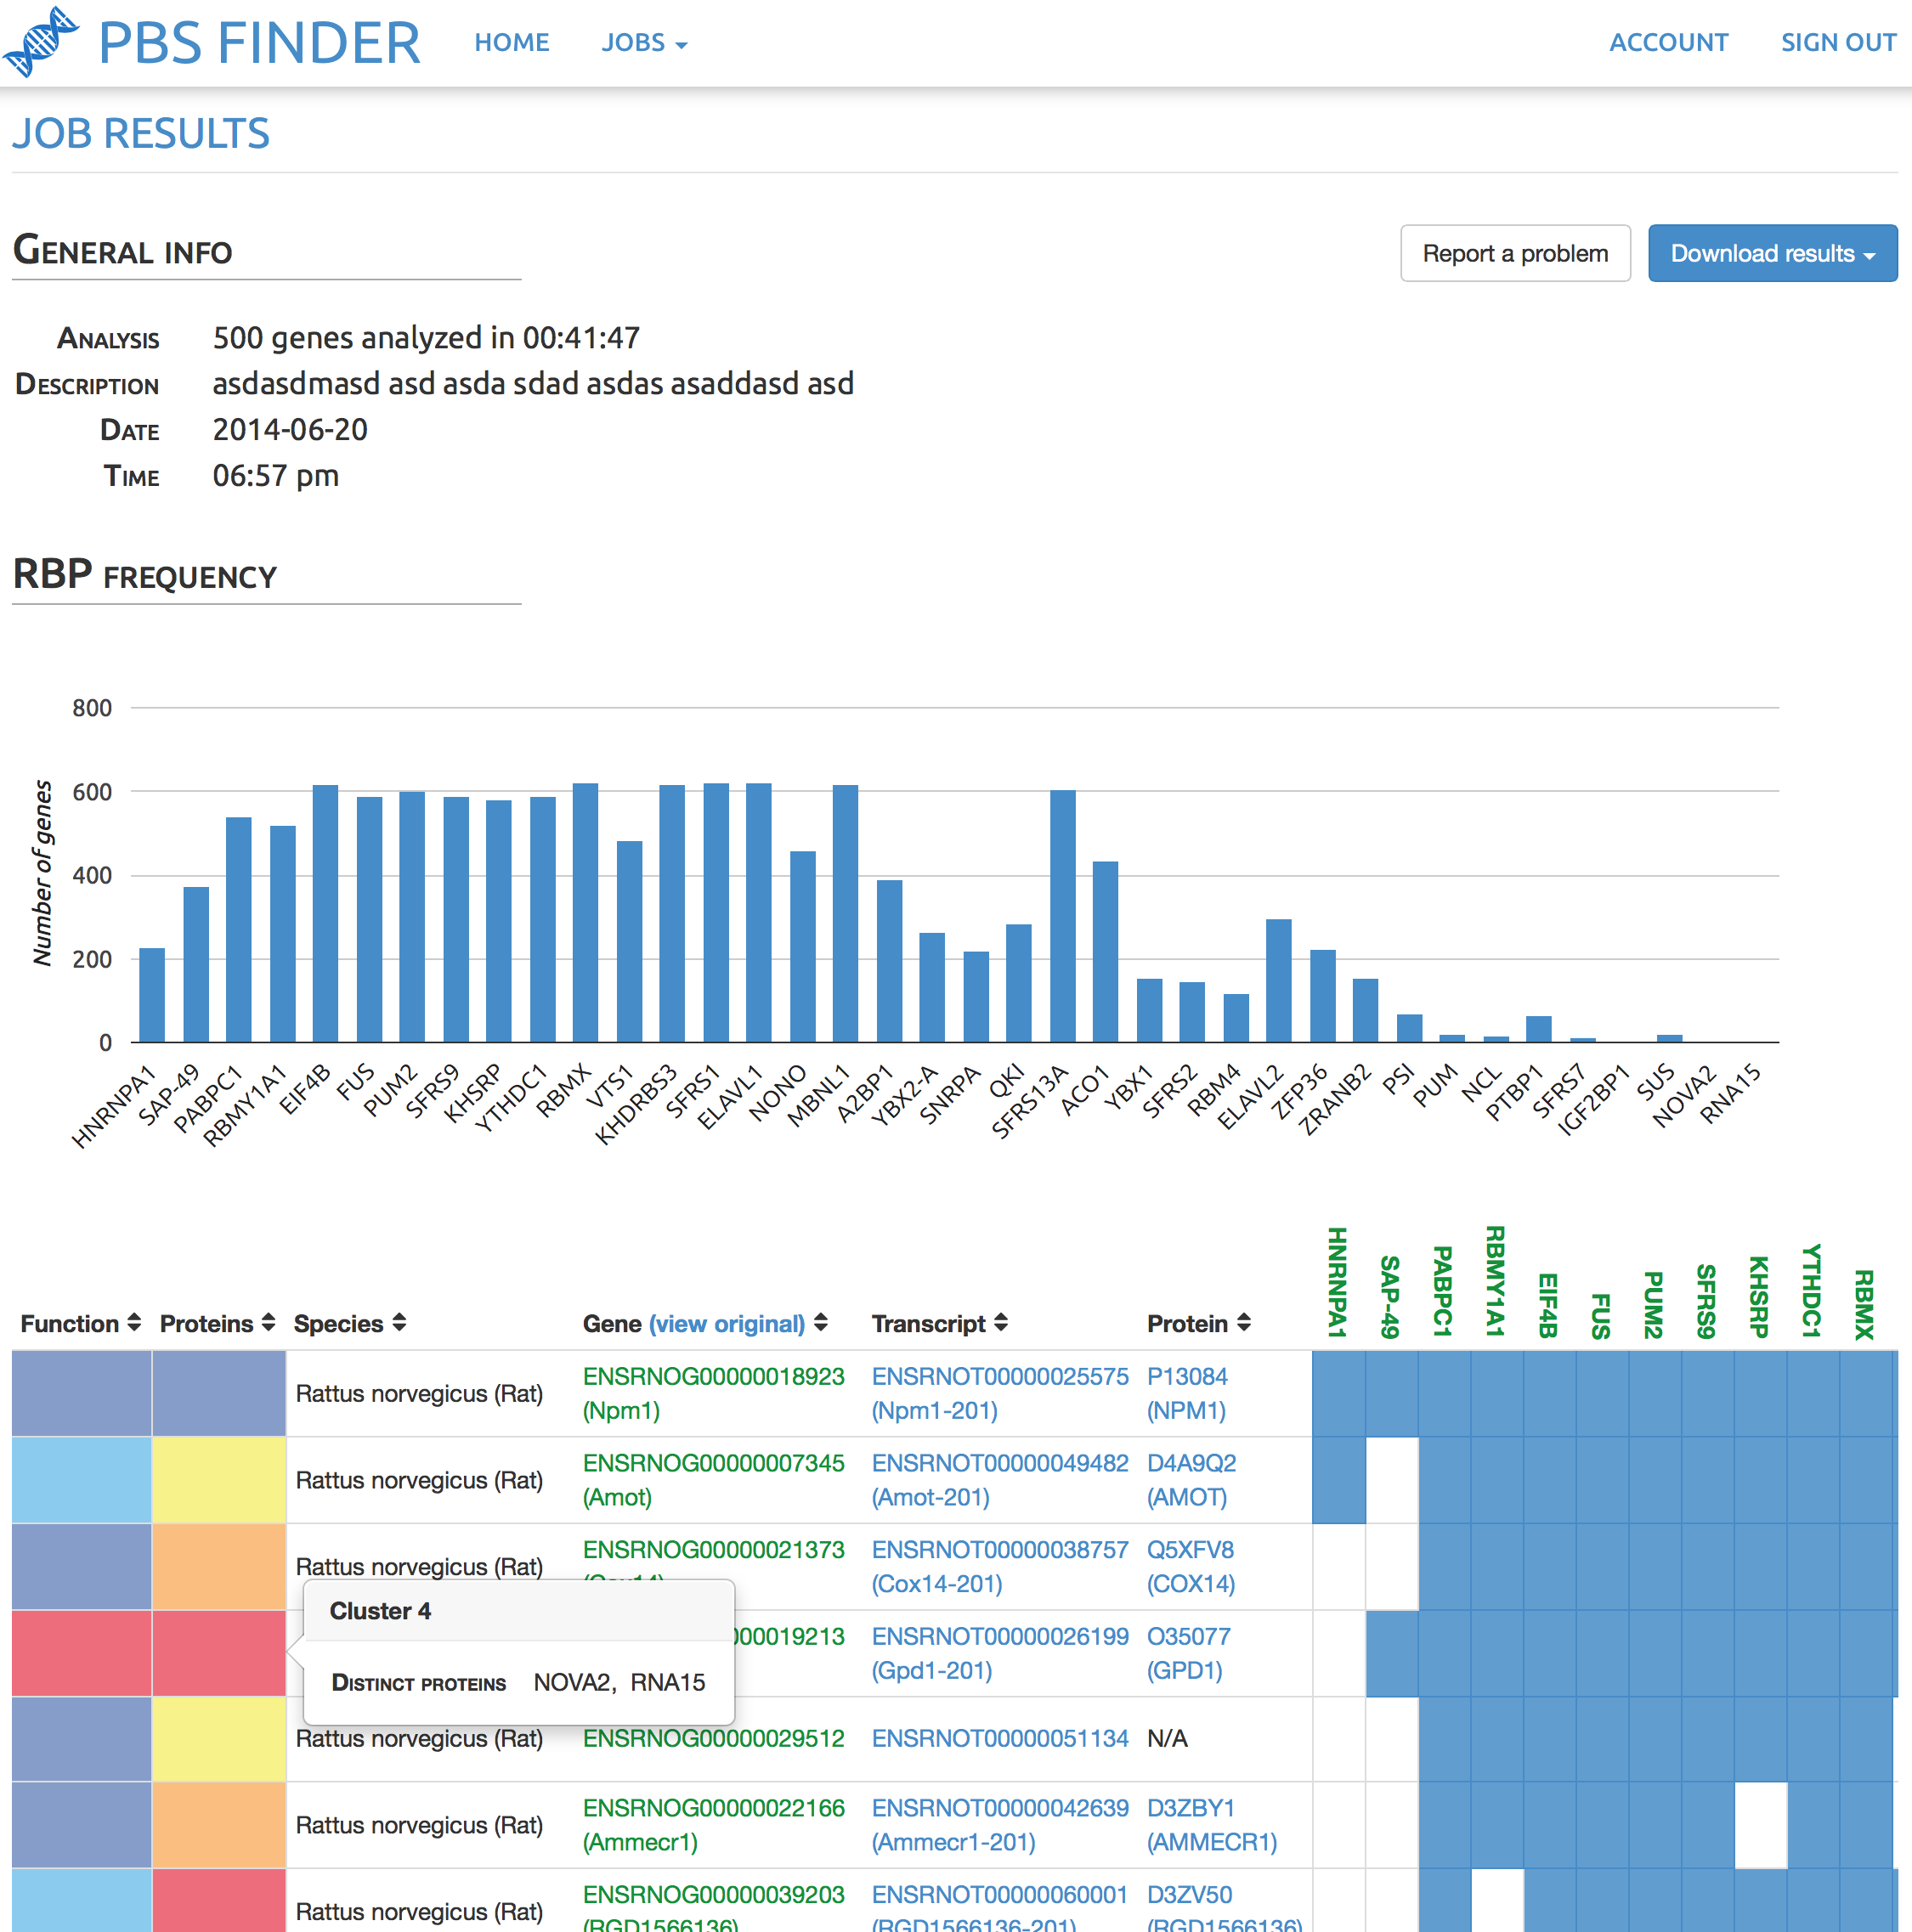
\includegraphics[width=\textwidth]{job_view}
    \caption[Job view example]{
      Job view example, also known as main view. It is comprised by three main
      components: general information (which includes data download); RBP
      frequency histogram; and RNA binding protein matching table.
    }
    \label{fig:job_view}
  \end{center}
\end{figure}

\begin{figure}[!htb]
  \begin{center}
    \leavevmode
    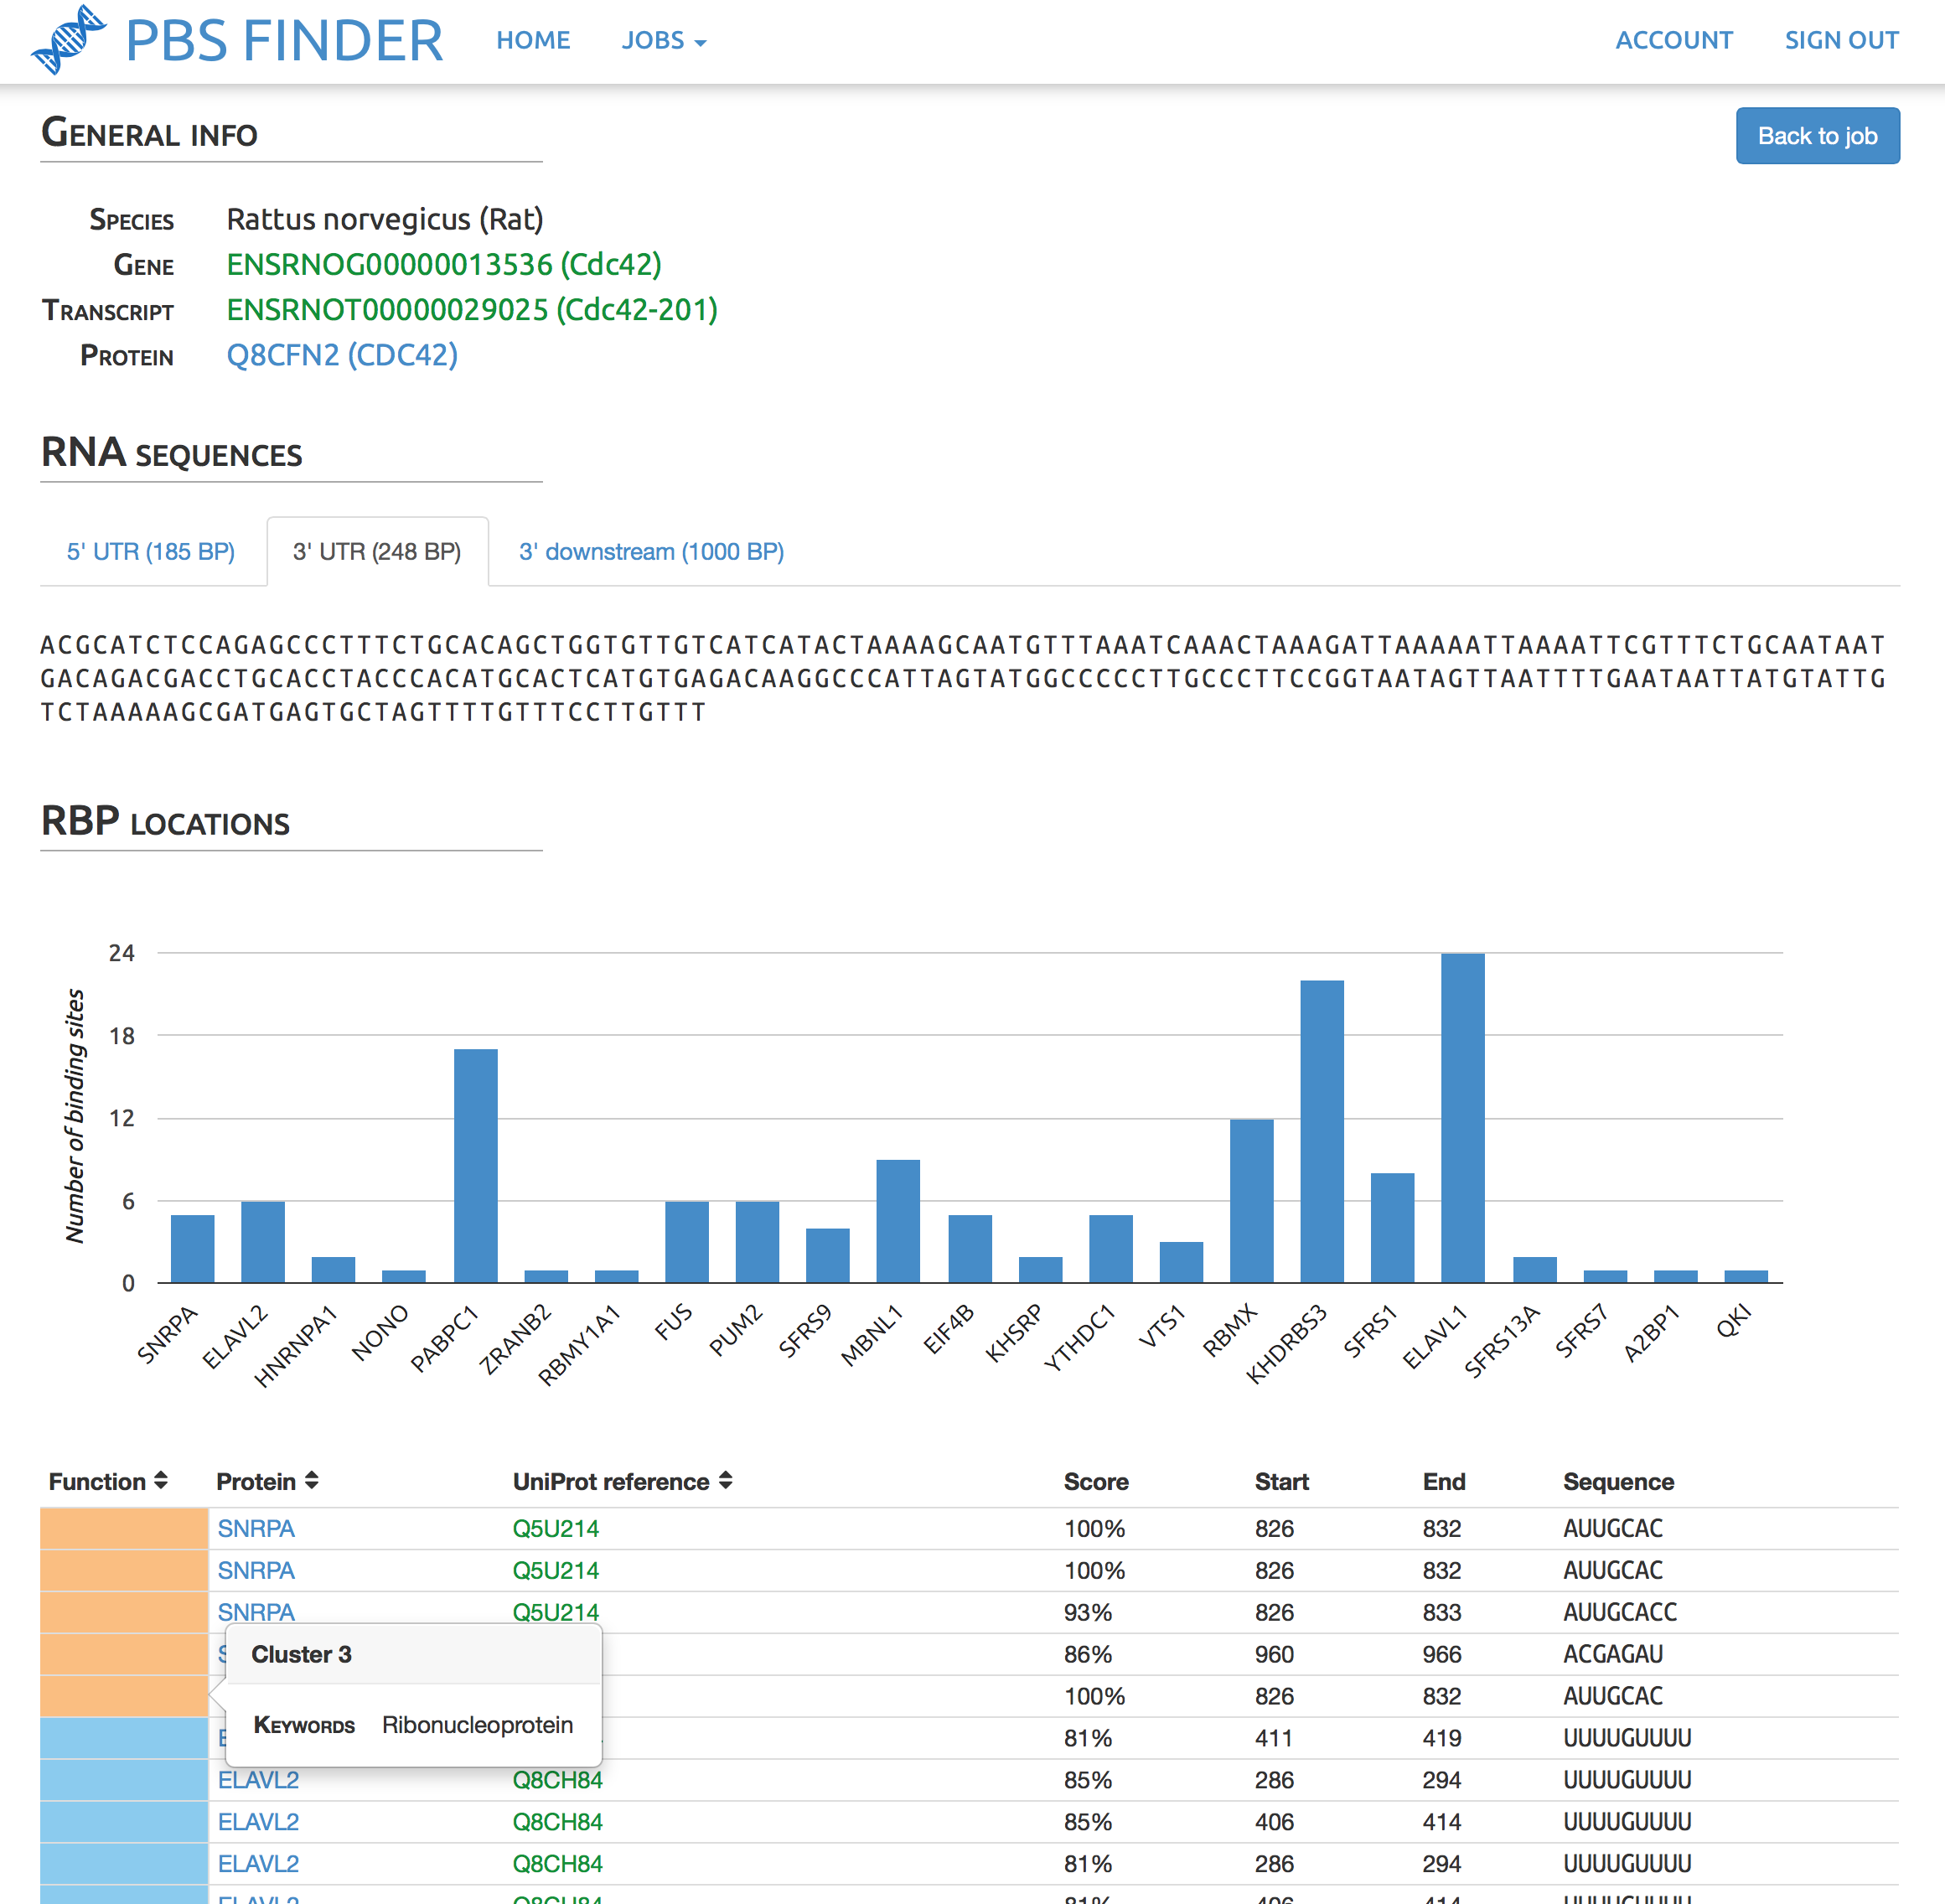
\includegraphics[width=\textwidth]{trans_view}
    \caption[Transcript view example]{
      Transcript view example. It contains four main areas: general information
      about the transcript; RNA sequences (5’UTR, 3’UTR and 3’UTR downstream are
      shown depending on availability); RBP locations histogram; and RBP
      location table (including clustering results and match sequences).
    }
    \label{fig:trans_view}
  \end{center}
\end{figure}

\begin{figure}[!htb]
  \begin{center}
    \leavevmode
    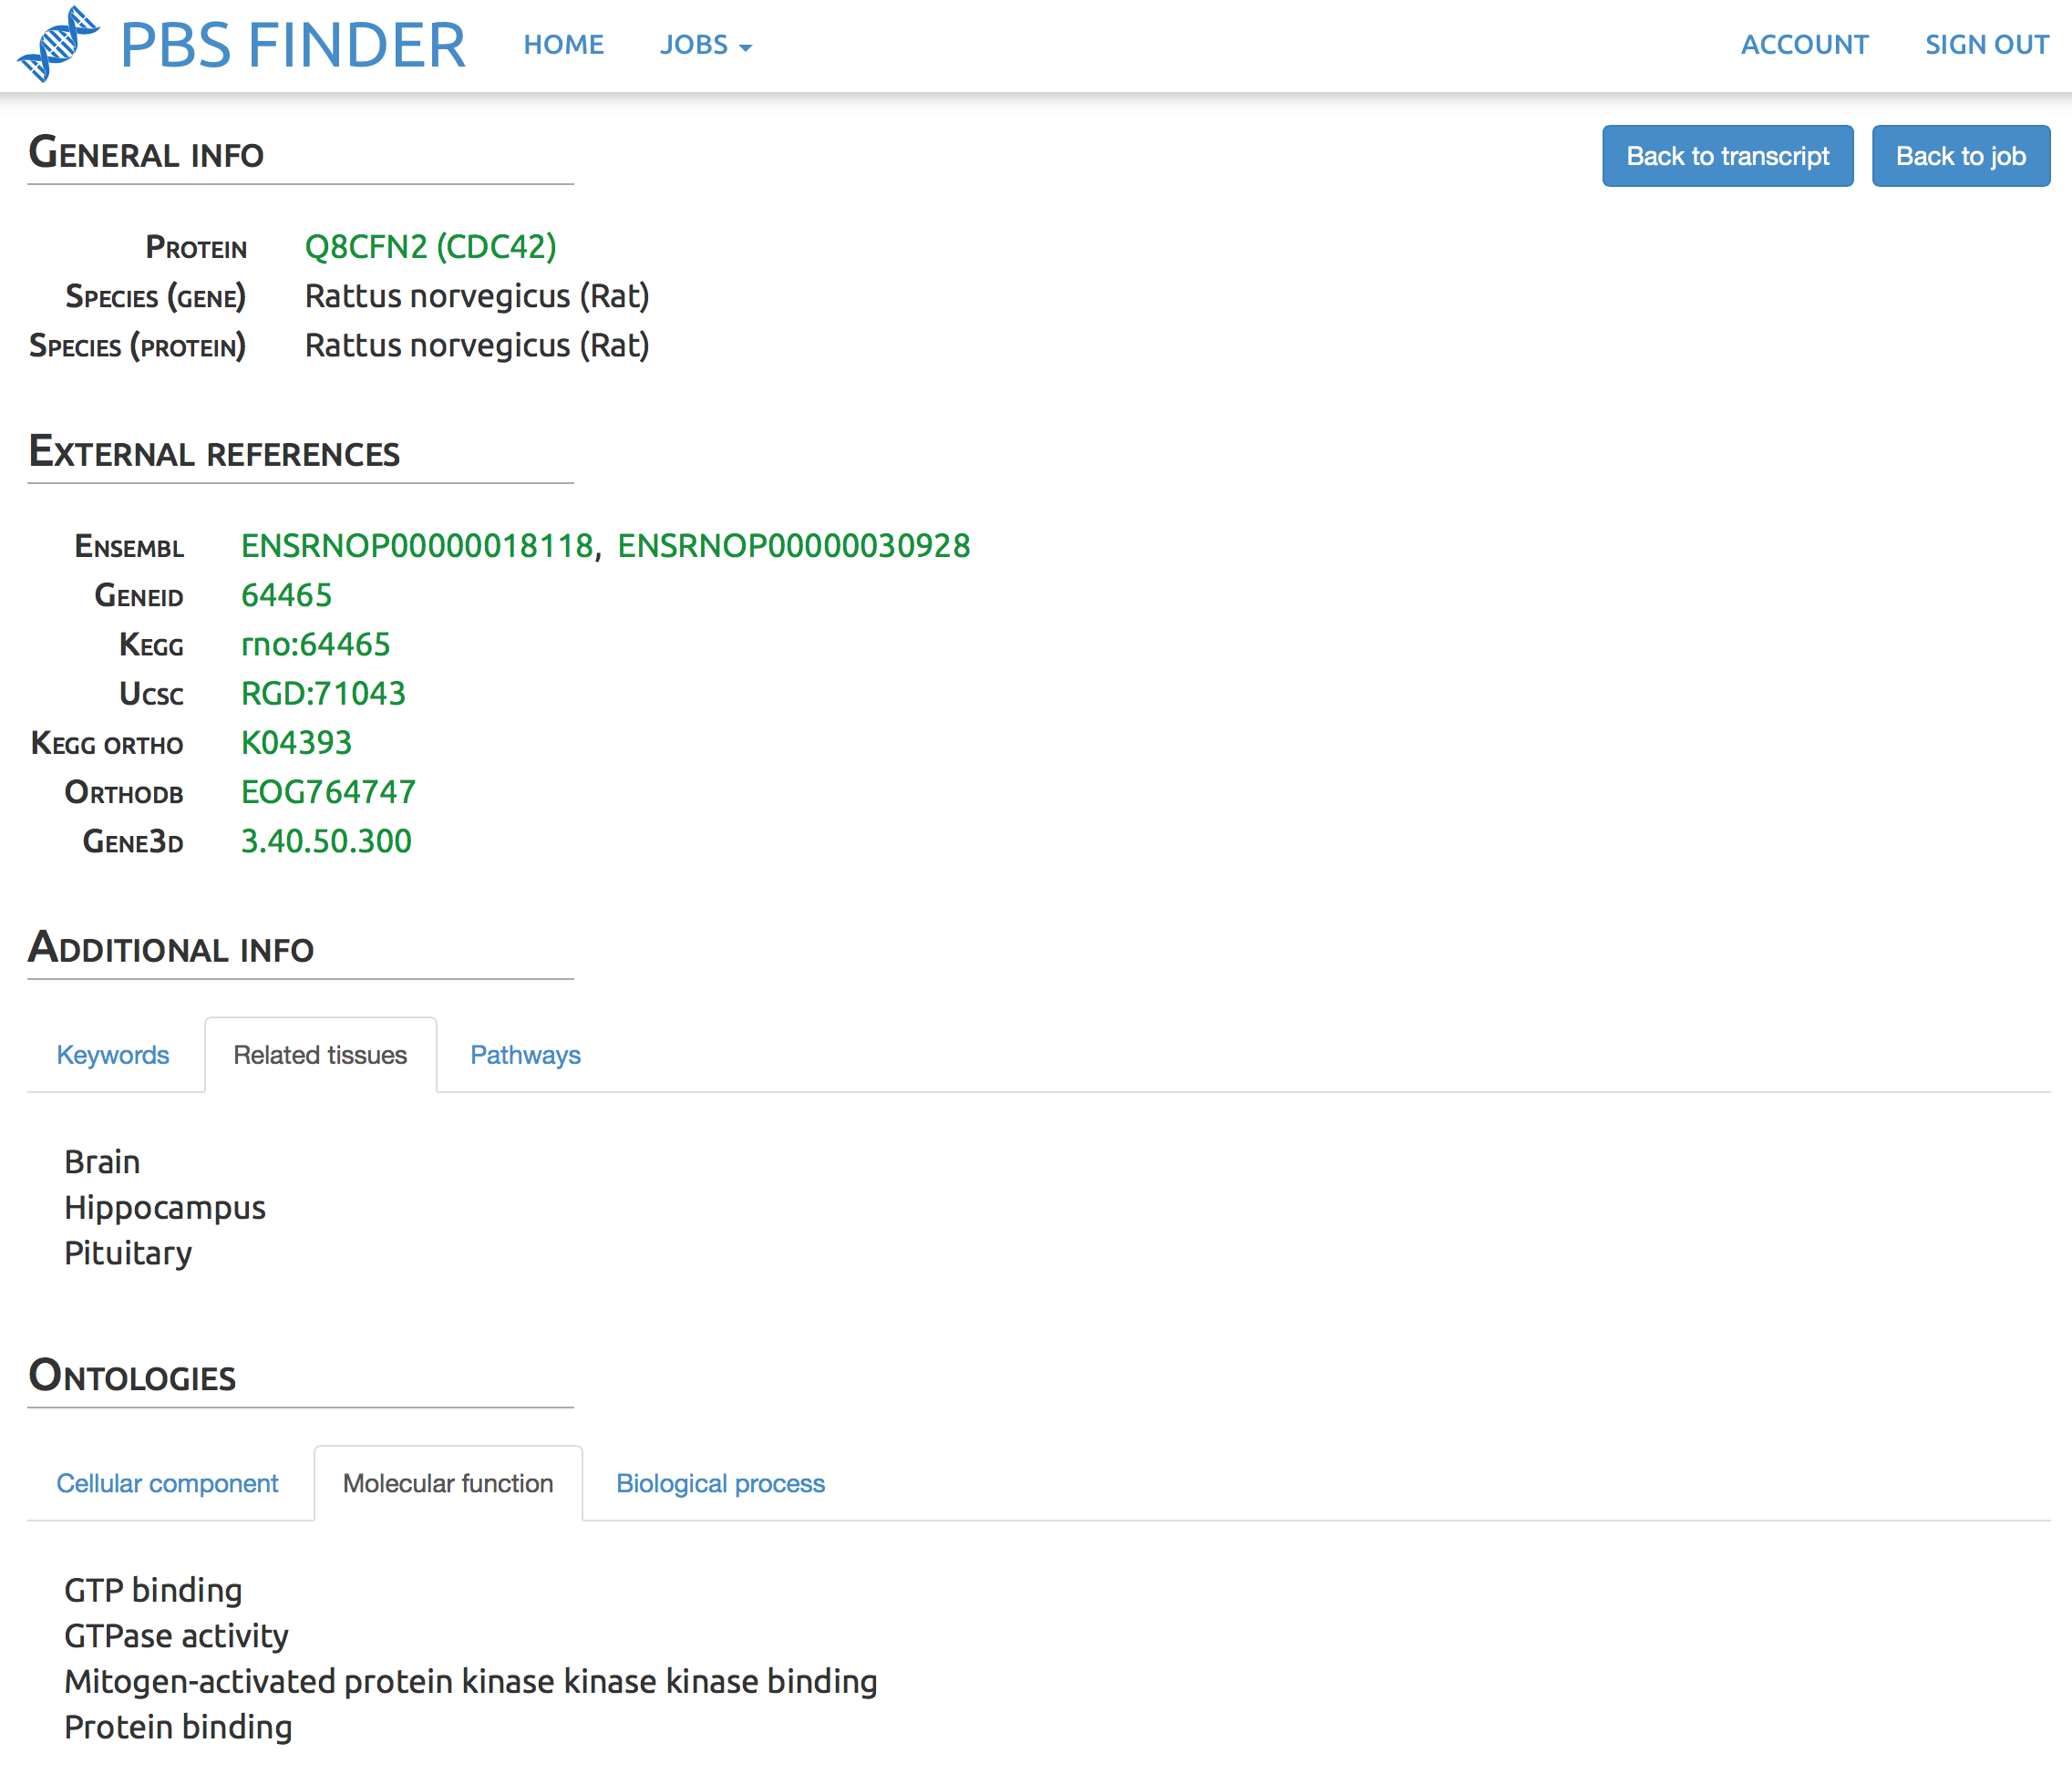
\includegraphics[width=\textwidth]{prot_view}
    \caption[Protein view example]{
      Protein view example, containing four relevant areas: general information
      about the protein; links to other web platforms with relevant information
      about the protein (note that some of those platforms might not contain
      information about a particular protein, and therefore no links can be
      shown); additional info, including keywords, related tissues and pathways
      in which the protein is expressed; and lastly, information about the
      protein's ontologies, including cellular components, molecular functions
      and biological processes.
    }
    \label{fig:prot_view}
  \end{center}
\end{figure}



\chapter{iRAP Example Configuration}\label{appendix:irapconfig}

\begin{lstlisting}[numbers=none, breaklines=true]
  # =============================================================================
  # Name of the experiment. (no spaces)
  # All files produced by irap will be placed in a folder with the given name.
  name=myexp

  # =============================================================================
  # Name of the species.
  species=homo_sapiens

  # =============================================================================
  # FASTA file with the reference genome.
  reference=Homo_sapiens.GRCh37.66.dna.fa

  # =============================================================================
  # GTF file with the annotations.
  gtf_file=Homo_sapiens.GRCh37.66.gtf

  # =============================================================================
  # iRAP options (may be provided in the command line).

  # Mapper
  # mapper=<pick one supported by iRAP>

  # Quantification method
  # quant_method=<pick one supported by iRAP>

  # Differential expression method
  # de_method=<pick one supported by iRAP>

  # Gene set enrichment (GSE) analysis
  # gse_tool=piano

  # Check data (reads) quality (on|off)
  # qual_filtering=on

  # Trim all reads to the minimum read size after quality trimming (y|n)
  # (only applicable if qual_filtering is on)
  # trim_reads=y

  # Minimum base quality accepted (default is 10)
  # min_read_quality=10

  # Contamination check (cont_index parameter).  Reads that likely originate from
  # organisms other than the one under study can be discarded during
  # pre-processment of the reads. This is done by aligning the reads to the
  # genomes of organisms that might be a source of contamination and discard
  # those that map with a high degree of fidelity. By default iRAP will check if
  # the data is contaminated by e-coli. An example to create a contamination
  # "database" is provided in the examples/ex_add2contaminationDB.sh script. The
  # value of the parameter should be the file name prefix of the bowtie index
  # files.

  # Disable contamination check
  # cont_index=no

  # Default value
  # cont_index=$(data_dir)/contamination/e_coli

  ###########################################
  # Miscellanious options

  # Number of threads that may be used by iRAP
  # max_threads=1

  # Exon level quantification (y|n)
  # exon_quant=y

  # Transcript level quantification (y|n)
  # transcript_quant=y

  # =============================================================================
  # Full or relative path to the directory where all the data can be found.
  data_dir=data

  # =============================================================================
  # Only necessary if you intend to perform Differential Expression analysis.

  # Contrasts
  contrasts=purpleVsPink purpleVsGrey

  # Definition of each constrast
  purlpleVsPink=Purple Pink
  purlpleVsGrey=Purple Grey

  # Groups definition
  Purlple=myLib1 myLib2
  Pink=myLib3
  Grey=myLib4

  # Technical replicates
  technical.replicates="myLib1,myLib2;myLib3;mylib4"

  # =============================================================================
  # Data
  # *_rs      => read size
  # *_qual    => quality encoding (33|64)
  # *_sd      => standard deviation
  # *_ins     => insert size

  myLib1=f1.fastq
  myLib1_rs=75
  myLib1_qual=33

  myLib2=f2.fastq
  myLib2_rs=75
  myLib2_qual=33

  myLib3=f3_1.fastq f3_2.fastq
  myLib3_rs=50
  myLib3_qual=33
  myLib3_ins=350
  myLib3_sd=60

  myLib4=f4_1.fastq f4_2.fastq
  myLib4_rs=50
  myLib4_qual=33
  myLib4_ins=350
  myLib4_sd=60

  # List the names of your single-end (se) and paired (pe) libraries
  se=myLib1 myLib2
  pe=myLib3 myLib4
\end{lstlisting}

\chapter{Examples of Biological Information Files}\label{annex:formats}

\section{SAM Example}
\begin{lstlisting}[numbers=none, breaklines=true]
  HD	VN:1.0 SO:coordinate
  @SQ	SN:seq1	LN:5000
  @SQ	SN:seq2	LN:5000
  @CO	Example of SAM/BAM file format.
  B7_591:4:96:693:509	73	seq1	1	99	36M	*	0	0	CACTAGTGGCTCATTGTAAATGTGTGGTTTAACTCG	<<<<<<<<<<<<<<<;<<<<<<<<<5<<<<<;:<;7	MF:i:18	Aq:i:73	NM:i:0	UQ:i:0	H0:i:1	H1:i:0
  EAS54_65:7:152:368:113	73	seq1	3	99	35M	*	0	0	CTAGTGGCTCATTGTAAATGTGTGGTTTAACTCGT	<<<<<<<<<<0<<<<655<<7<<<:9<<3/:<6):	MF:i:18	Aq:i:66	NM:i:0	UQ:i:0	H0:i:1	H1:i:0
  EAS51_64:8:5:734:57	137	seq1	5	99	35M	*	0	0	AGTGGCTCATTGTAAATGTGTGGTTTAACTCGTCC	<<<<<<<<<<<7;71<<;<;;<7;<<3;);3*8/5	MF:i:18	Aq:i:66	NM:i:0	UQ:i:0	H0:i:1	H1:i:0
  B7_591:1:289:587:906	137	seq1	6	63	36M	*	0	0	GTGGCTCATTGTAATTTTTTGTTTTAACTCTTCTCT	(-&----,----)-)-),'--)---',+-,),''*,	MF:i:130	Aq:i:63	NM:i:5	UQ:i:38	H0:i:0	H1:i:0
  EAS56_59:8:38:671:758	137	seq1	9	99	35M	*	0	0	GCTCATTGTAAATGTGTGGTTTAACTCGTCCATGG	<<<<<<<<<<<<<<<;<;7<<<<<<<<7<<;:<5%	MF:i:18	Aq:i:72	NM:i:0	UQ:i:0	H0:i:1	H1:i:0
  EAS56_61:6:18:467:281	73	seq1	13	99	35M	*	0	0	ATTGTAAATGTGTGGTTTAACTCGTCCCTGGCCCA	<<<<<<<<;<<<8<<<<<;8:;6/686&;(16666	MF:i:18	Aq:i:39	NM:i:1	UQ:i:5	H0:i:0	H1:i:1
  EAS114_28:5:296:340:699	137	seq1	13	99	36M	*	0	0	ATTGTAAATGTGTGGTTTAACTCGTCCATGGCCCAG	<<<<<;<<<;<;<<<<<<<<<<<8<8<3<8;<;<0;	MF:i:18	Aq:i:73	NM:i:0	UQ:i:0	H0:i:1	H1:i:0
\end{lstlisting}

\section{VCF Example}
\begin{lstlisting}[numbers=none, breaklines=true]
  ##fileformat=VCFv4.0
  ##fileDate=20090805
  ##source=myImputationProgramV3.1
  ##reference=1000GenomesPilot-NCBI36
  ##phasing=partial
  ##INFO=<ID=NS,Number=1,Type=Integer,Description="Number of Samples With Data">
  ##INFO=<ID=DP,Number=1,Type=Integer,Description="Total Depth">
  ##INFO=<ID=AF,Number=.,Type=Float,Description="Allele Frequency">
  ##INFO=<ID=AA,Number=1,Type=String,Description="Ancestral Allele">
  ##INFO=<ID=DB,Number=0,Type=Flag,Description="dbSNP membership, build 129">
  ##INFO=<ID=H2,Number=0,Type=Flag,Description="HapMap2 membership">
  ##FILTER=<ID=q10,Description="Quality below 10">
  ##FILTER=<ID=s50,Description="Less than 50% of samples have data">
  ##FORMAT=<ID=GT,Number=1,Type=String,Description="Genotype">
  ##FORMAT=<ID=GQ,Number=1,Type=Integer,Description="Genotype Quality">
  ##FORMAT=<ID=DP,Number=1,Type=Integer,Description="Read Depth">
  ##FORMAT=<ID=HQ,Number=2,Type=Integer,Description="Haplotype Quality">
  #CHROM POS     ID        REF ALT    QUAL FILTER INFO                              FORMAT      NA00001        NA00002        NA00003
  20     14370   rs6054257 G      A       29   PASS   NS=3;DP=14;AF=0.5;DB;H2           GT:GQ:DP:HQ 0|0:48:1:51,51 1|0:48:8:51,51 1/1:43:5:.,.
  20     17330   .         T      A       3    q10    NS=3;DP=11;AF=0.017               GT:GQ:DP:HQ 0|0:49:3:58,50 0|1:3:5:65,3   0/0:41:3
  20     1110696 rs6040355 A      G,T     67   PASS   NS=2;DP=10;AF=0.333,0.667;AA=T;DB GT:GQ:DP:HQ 1|2:21:6:23,27 2|1:2:0:18,2   2/2:35:4
  20     1230237 .         T      .       47   PASS   NS=3;DP=13;AA=T                   GT:GQ:DP:HQ 0|0:54:7:56,60 0|0:48:4:51,51 0/0:61:2
  20     1234567 microsat1 GTCT   G,GTACT 50   PASS   NS=3;DP=9;AA=G                    GT:GQ:DP    0/1:35:4 
\end{lstlisting}

\section{FASTQ Example}
\begin{lstlisting}[numbers=none, breaklines=true]
  @SRR014849.1 EIXKN4201CFU84 length=93
  GGGGGGGGGGGGGGGGCTTTTTTTGTTTGGAACCGAAAGG
  GTTTTGAATTTCAAACCCTTTTCGGTTTCCAACCTTCCAA
  AGCAATGCCAATA
  +SRR014849.1 EIXKN4201CFU84 length=93
  3+&$#"""""""""""7F@71,’";C?,B;?6B;:EA1EA
  1EA5’9B:?:#9EA0D@2EA5’:>5?:%A;A8A;?9B;D@
  /=<?7=9<2A8==
\end{lstlisting}

\section{FASTA Example}
\begin{lstlisting}[numbers=none, breaklines=true]
  >gi|5524211|gb|AAD44166.1| cytochrome b [Elephas maximus maximus]
  LCLYTHIGRNIYYGSYLYSETWNTGIMLLLITMATAFMGYVLPWGQMSFWGATVITNLFSAIPYIGTNLV
  EWIWGGFSVDKATLNRFFAFHFILPFTMVALAGVHLTFLHETGSNNPLGLTSDSDKIPFHPYYTIKDFLG
  LLILILLLLLLALLSPDMLGDPDNHMPADPLNTPLHIKPEWYFLFAYAILRSVPNKLGGVLALFLSIVIL
  GLMPFLHTSKHRSMMLRPLSQALFWTLTMDLLTLTWIGSQPVEYPYTIIGQMASILYFSIILAFLPIAGX
  IENY
\end{lstlisting}

\section{GTF/GFF Example}
\begin{lstlisting}[numbers=none, breaklines=true]
  ## GFF
  ##gff-version 3
  ##sequence-region   ctg123 1 1497228
  ctg123 . gene            1000  9000  .  +  .  ID=gene00001;Name=EDEN
  ctg123 . TF_binding_site 1000  1012  .  +  .  ID=tfbs00001;Parent=gene00001
  ctg123 . mRNA            1050  9000  .  +  .  ID=mRNA00001;Parent=gene00001;Name=EDEN.1
  ctg123 . mRNA            1050  9000  .  +  .  ID=mRNA00002;Parent=gene00001;Name=EDEN.2
  ctg123 . mRNA            1300  9000  .  +  .  ID=mRNA00003;Parent=gene00001;Name=EDEN.3
  ctg123 . exon            1300  1500  .  +  .  ID=exon00001;Parent=mRNA00003
  ctg123 . exon            1050  1500  .  +  .  ID=exon00002;Parent=mRNA00001,mRNA00002
  ctg123 . exon            3000  3902  .  +  .  ID=exon00003;Parent=mRNA00001,mRNA00003

  ---------------------------------------------------

  ## GTF
  140    Twinscan    inter         5141     8522     .    -    .    gene_id ""; transcript_id "";
  140    Twinscan    inter_CNS     8523     9711     .    -    .    gene_id ""; transcript_id "";
  140    Twinscan    inter         9712     13182    .    -    .    gene_id ""; transcript_id "";
  140    Twinscan    3UTR          65149    65487    .    -    .    gene_id "140.000"; transcript_id "140.000.1";
  140    Twinscan    3UTR          66823    66992    .    -    .    gene_id "140.000"; transcript_id "140.000.1";
  140    Twinscan    stop_codon    66993    66995    .    -    0    gene_id "140.000"; transcript_id "140.000.1";
\end{lstlisting}


%% Index
%% Uncomment next command if index is required
%\PrintIndex

\end{document}
